\documentclass[sigconf]{acmart}
%\documentclass[sigconf,nonacm]{acmart}

\usepackage{booktabs} % For formal tables
\usepackage{amsmath,amssymb,amsfonts,amsthm}
\usepackage[english]{babel}
\usepackage{xcolor}
\usepackage{tikz}
\usetikzlibrary{automata, graphs,positioning,chains,arrows,decorations.pathmorphing}
\usepackage{url}
\usepackage{subcaption}

% Copyright
%\setcopyright{none}
%\setcopyright{acmcopyright}
%\setcopyright{acmlicensed}
%\setcopyright{rightsretained}
%\setcopyright{usgov}
%\setcopyright{usgovmixed}
%\setcopyright{cagov}
%\setcopyright{cagovmixed}


% DOI
%\acmDOI{10.475/123_4}

% ISBN
%\acmISBN{123-4567-24-567/08/06}

%Conference
%\acmConference[WOODSTOCK'97]{ACM Woodstock conference}{July 1997}{El
%  Paso, Texas USA}
%\acmYear{1997}
%\copyrightyear{2016}


%\acmArticle{4}
%\acmPrice{15.00}

% These commands are optional
%\acmBooktitle{Transactions of the ACM Woodstock conference}
%\editor{Jennifer B. Sartor}
%\editor{Theo D'Hondt}
%\editor{Wolfgang De Meuter}

%% Macros Juan

\newcommand{\paths}{\text{PATHS}}

%% Macros comments
\newcommand{\tover}[1]{\textcolor{red}{#1}}
\newcommand{\td}[1]{\textcolor{blue}{[TODO: #1]}}

%% Macros logics
\newcommand{\NN}{\mathbb{N}}
\newcommand{\ZZ}{\mathbb{Z}}
\newcommand{\MM}{\mathbb{M}}
\newcommand{\SE}{\mathbb{S}}
\newcommand{\BB}{\mathbb{B}}
\newcommand{\RR}{\mathbb{R}}
\newcommand{\cF}{\mathcal{F}}
\newcommand{\cI}{\mathcal{I}}
\newcommand{\QFBILIA}{\textsf{QFBILIA}}
\newcommand{\nnf}{\textsf{f}}

\newcommand{\ite}{\textsf{ite}}
\newcommand{\limp}{\Rightarrow}
\newcommand{\flc}{\rightarrow}

\newcommand{\bagone}[1]{\llbracket #1 \rrbracket}
\newcommand{\bsingle}{\textsf{bag}}
\newcommand{\bplus}{\oplus}
\newcommand{\bminus}{\ominus}

%% Macros tools
\newcommand{\spen}{\textsc{spen}}
\newcommand{\zzz}{\textsc{Z3}}

%% Environments
\newtheorem{mythm}{Theorem}[section]
\newtheorem{mydef}[mythm]{Definition}
\newtheorem{myprop}[mythm]{Proposition}
\newtheorem{mylem}[mythm]{Lemma}
\newtheorem{myex}[mythm]{Example}
\newtheorem{mycor}[mythm]{Corollary}

\newtheorem*{myrem}{Remark} %% based on amsthm
\newtheorem*{mynota}{Notation}
\newtheorem*{mylem*}{Lemma}
\newtheorem{myclaim}{Claim}
\newtheorem*{myclaim*}{Claim}
\newtheorem*{myprop*}{Proposition}
\newtheorem*{comp}{Efficiency Study}


\newenvironment{point}[1]
{\subsection*{#1}}%
{}

\newcommand{\flist}{\text{\sc FList}}
\newcommand{\set}{\text{\sc Set}}
\newcommand{\fset}{\text{\sc FSet}}
\newcommand{\B}{\text{\bf B}}
%\newcommand{\G}{\mathcal{G}}
\newcommand{\K}{\mathcal{K}}
\newcommand{\LOG}{\text{\sc Log}}
\newcommand{\length}{\text{\rm length}}
\newcommand{\BK}{\text{\sc BK}}
%\newcommand{\cP}{\mathcal{P}}
%\newcommand{\cV}{\mathcal{V}}
%\newcommand{\cC}{\mathcal{C}}
%\newcommand{\cS}{\mathcal{S}}
%\newcommand{\cA}{\mathcal{A}}
%\newcommand{\cR}{\mathcal{R}}
%\newcommand{\cQ}{\mathcal{Q}}
\newcommand{\cG}{\mathcal{G}}
\newcommand{\cT}{\mathcal{T}}
\newcommand{\pr}{\mathbf{Pr}}
\newcommand{\Dyck}{\mathcal{D}}
\newcommand{\expected}{\mathbf{E}}
\newcommand{\bv}{\mathbf{v}}
\newcommand{\bV}{\mathbf{V}}
\newcommand{\bs}{\mathbf{s}}
\newcommand{\bsigma}{\mathbf{\sigma}}
\newcommand{\bw}{\mathbf{w}}
\newcommand{\ba}{\mathbf{a}}
\newcommand{\bq}{\mathbf{q}}
\newcommand{\bx}{\mathbf{x}}
\newcommand{\by}{\mathbf{y}}

\newcommand{\bstring}{\{0,1\}^\ast}

\newcommand{\marcelo}[1]{{\color{red} {\bf Marcelo: #1}}}
\newcommand{\etienne}[1]{{\color{blue} {\bf Etienne: #1}}}
\newcommand{\juan}[1]{{\textcolor{violet} {\bf Juan: #1}}}
\newcommand{\domagoj}[1]{{\color{green} {\bf Domagoj: #1}}}
\newcommand{\francisco}[1]{{\color{magenta} {\bf Francisco: #1}}}
\newcommand{\martin}[1]{{\color{orange} {\bf Martin: #1}}}

\newcommand{\quot}[1]{#1/\!\equiv}

\newcommand{\then}{\,|\,}
\newcommand{\body}{q}
\newcommand{\bchain}{\text{bc}}
\newcommand{\epath}{\text{path}}

\newcommand{\owner}{\text{\rm owner}}
\newcommand{\pred}{\text{\rm pred}}
\newcommand{\mine}{\text{\rm mine}}
\newcommand{\suc}{\text{\rm succ}}


\newcommand{\bP}{\mathbf{P}}
\newcommand{\bB}{\mathbf{B}}
\newcommand{\bA}{\mathbf{A}}
\newcommand{\bR}{\mathbf{R}}
\newcommand{\bS}{\mathbf{S}}
\newcommand{\bH}{\mathbf{H}}
\newcommand{\bQ}{\mathbf{Q}}

\newcommand{\forkm}[1]{F^{#1}}
\newcommand{\mfork}{F_m}
\newcommand{\mgfork}{F_{m,g}}
\newcommand{\last}{\text{\rm last}}
\newcommand{\best}{\text{\rm best}}
\newcommand{\cho}{\text{\rm choose}}

\newcommand{\ie}{i.e.$\!$ }

\newcommand{\longest}{{\text{\rm longest}}}


\newcommand{\subbody}{{\text{\rm sub-state}}}

\newcommand{\cdf}{\text{\rm {\bf DF}}}
\newcommand{\df}{\text{\rm DF}}
\newcommand{\fg}{\text{\rm FG}}
\newcommand{\fr}{\text{\rm FR}}
\newcommand{\bdf}{\text{\rm {\bf DF}}}
\newcommand{\bfg}{\text{\rm {\bf FG}}}
\newcommand{\bfr}{\text{\rm {\bf FR}}}


%\newcommand{\af}{{\rm {F_\infty}}}
%\newcommand{\baf}{{\rm {\bf F_\infty}}}

\newcommand{\af}{\text{\rm AF}}
\newcommand{\baf}{\text{\rm {\bf AF}}}

\newcommand{\pf}[1]{\text{\rm F[{#1}]}}
\newcommand{\bpf}[1]{\text{\rm {\bf F}[{$#1$}]}}

\newcommand{\cat}{\text{\rm Catalan}}


\newcommand{\gup}{{\rm {G}}}
\newcommand{\bgup}{{\rm {\bf G}}}


\newcommand{\catalan}{{\rm {\it C}}}
%\newcommand{\dyck}{{\rm {\it D}}}


\newcommand{\meet}{\text{\rm meet}}

\DeclareMathOperator*{\argmax}{argmax}


%\newcommand{\rpa}{r_p^\alpha}
\newcommand{\rpa}{r_p}

\newcommand{\ameet}{\text{\rm all-meet}}
\newcommand{\base}{\text{\rm base}}

\newcommand{\ucl}{\text{\rm up-cl}}
\newcommand{\dcl}{\text{\rm down-cl}}

\newcommand{\pol}{\text{\it P}}





\allowdisplaybreaks

\begin{document}
%\title{Should I fork? \\ A formal look at mining in cryptocurrencies.}
%\title{Should I fork? \\ Cryptocurrencies mining as a stoshastic game.}
%\title{Should I fork? \\Cryptocurrency mining through a stochastic stethoscope}
%\title{Cryptocurrency mining through a stochastic stethoscope}
\title{Cryptocurrency Mining through Stochastic Lenses}
%\title{Formal foundations of cryptocurrency mining} %PLEASE NOT THIS ONE
%\titlenote{Produces the permission block, and
%  copyright information}
%\subtitle{Extended Abstract}
%\subtitlenote{The full version of the author's guide is available as
%  \texttt{acmart.pdf} document}


%\author{Ben Trovato}
%\authornote{Dr.~Trovato insisted his name be first.}
%\orcid{1234-5678-9012}
%\affiliation{%
%  \institution{Institute for Clarity in Documentation}
%  \streetaddress{P.O. Box 1212}
%  \city{Dublin}
%  \state{Ohio}
%  \postcode{43017-6221}
%}
%\email{trovato@corporation.com}
%
%\author{G.K.M. Tobin}
%\authornote{The secretary disavows any knowledge of this author's actions.}
%\affiliation{%
%  \institution{Institute for Clarity in Documentation}
%  \streetaddress{P.O. Box 1212}
%  \city{Dublin}
%  \state{Ohio}
%  \postcode{43017-6221}
%}
%\email{webmaster@marysville-ohio.com}
%
%\author{Lars Th{\o}rv{\"a}ld}
%\authornote{This author is the
%  one who did all the really hard work.}
%\affiliation{%
%  \institution{The Th{\o}rv{\"a}ld Group}
%  \streetaddress{1 Th{\o}rv{\"a}ld Circle}
%  \city{Hekla}
%  \country{Iceland}}
%\email{larst@affiliation.org}
%
%\author{Valerie B\'eranger}
%\affiliation{%
%  \institution{Inria Paris-Rocquencourt}
%  \city{Rocquencourt}
%  \country{France}
%}
%\author{Aparna Patel}
%\affiliation{%
% \institution{Rajiv Gandhi University}
% \streetaddress{Rono-Hills}
% \city{Doimukh}
% \state{Arunachal Pradesh}
% \country{India}}
%\author{Huifen Chan}
%\affiliation{%
%  \institution{Tsinghua University}
%  \streetaddress{30 Shuangqing Rd}
%  \city{Haidian Qu}
%  \state{Beijing Shi}
%  \country{China}
%}
%
%\author{Charles Palmer}
%\affiliation{%
%  \institution{Palmer Research Laboratories}
%  \streetaddress{8600 Datapoint Drive}
%  \city{San Antonio}
%  \state{Texas}
%  \postcode{78229}}
%\email{cpalmer@prl.com}
%
%\author{John Smith}
%\affiliation{\institution{The Th{\o}rv{\"a}ld Group}}
%\email{jsmith@affiliation.org}
%
%\author{Julius P.~Kumquat}
%\affiliation{\institution{The Kumquat Consortium}}
%\email{jpkumquat@consortium.net}
%
%% The default list of authors is too long for headers.
%\renewcommand{\shortauthors}{B. Trovato et al.}


\begin{abstract}
In the consensus protocol used in most cryptocurrencies, participants are expected to perform actions for which they receive a reward. 
These actions are colloquially known as mining, and protocols must ensure that mining is reward-compatible: participants are expected to behave correctly if they want to maximise their gains. %Yet studying incentives behind mining actions in cryptocurrencies has proven a difficult task, as protocols are full of details and  technicalities. We are thus left without a clear understanding of the miner's incentives and their optimal behaviour, and most of what is currently know is based solely on trial and error. 
Yet studying incentives behind mining actions in cryptocurrencies has proven a difficult task, leaving us without a clear understanding of optimal miner behaviour. %, or the precise value of the incentives in cryptocurrency protocols. 

Our goal is to understand how do optimal mining strategies look like, and particularly under which circumstances are miners incentivised to fork the blockchain by mining on top of blocks which are not at the tail of the current chain.  We model mining in cryptocurrencies as a stochastic game in which players always try to 
produce new blocks, and are rewarded for it. The probability of a player producing a new block depends on the hash power of the player, that is, the proportion of the computational power he controls compared to the power of the entire network. Players then look to maximise their utility in the long run, and their best strategy depends on their hash power and the discount 
applied to the reward of each new block being mined. 
We show that if no discount is offered, then miners do not have any incentive to fork, no matter how high their hash power is. On the other hand, when working with 
discounts similar to those in Bitcoin, miners do have an incentive to fork; in fact, they may want to do so even when they own less than half of the network's hash power. 
\end{abstract}

%
% The code below should be generated by the tool at
% http://dl.acm.org/ccs.cfm
% Please copy and paste the code instead of the example below.
%
%\begin{CCSXML}
%<ccs2012>
% <concept>
%  <concept_id>10010520.10010553.10010562</concept_id>
%  <concept_desc>Computer systems organization~Embedded systems</concept_desc>
%  <concept_significance>500</concept_significance>
% </concept>
% <concept>
%  <concept_id>10010520.10010575.10010755</concept_id>
%  <concept_desc>Computer systems organization~Redundancy</concept_desc>
%  <concept_significance>300</concept_significance>
% </concept>
% <concept>
%  <concept_id>10010520.10010553.10010554</concept_id>
%  <concept_desc>Computer systems organization~Robotics</concept_desc>
%  <concept_significance>100</concept_significance>
% </concept>
% <concept>
%  <concept_id>10003033.10003083.10003095</concept_id>
%  <concept_desc>Networks~Network reliability</concept_desc>
%  <concept_significance>100</concept_significance>
% </concept>
%</ccs2012>
%\end{CCSXML}
%
%\ccsdesc[500]{Computer systems organization~Embedded systems}
%\ccsdesc[300]{Computer systems organization~Redundancy}
%\ccsdesc{Computer systems organization~Robotics}
%\ccsdesc[100]{Networks~Network reliability}
%
%
%\keywords{ACM proceedings, \LaTeX, text tagging}


\maketitle

%\input{samplebody-conf}

	%!TEX root = main.tex

\section{Introduction}

The Bitcoin Protocol \cite{Bitcoin,DBLP:books/daglib/0040621,NC17}, or Nakamoto Protocol, introduces a novel decentralized network-consensus mechanism that is trustless and open for anyone connected to the Internet. To support such an open and dynamic topology, the protocol requires an underlying currency (a so-called \emph{cryptocurrency} \cite{NC17}) to encourage/discourage participants to/from taking certain actions. The largest network running this protocol at the time of writing is the Bitcoin network, and its underlying cryptocurrency is Bitcoin (BTC). Following the success of Bitcoin, several new cryptocurrencies have been created. Some of them are based on a simple replicas of Bitcoin with slight modifications on the protocol parameters (e.g. Litecoin~\cite{Litecoin} or Bitcoin Cash~\cite{Bcash}), while some of them introduce interesting new modifications on top of the protocol to provide further functionalities (e.g. Ethereum~\cite{Ethereum,E17} or Monero~\cite{Monero}). 
 
However, despite the success and popularity of cryptocurrencies, the foundational aspects of their ruling protocols are far from being fully understood. As it has been claimed before \cite{mininggames:2016}, the Bitcoin protocol involves many actors and incentives, making it rather hard to formalize and study rigorously. Our goal in this paper is to construct a model that will both allow us to have a clean understanding of actors and incentives in a cryptocurrency protocol, and to analyse the implications and consequences of future modifications to the  protocol. In doing so, we focus on the action of cryptocurrency \emph{mining}, as this will allow us to gauge the impact of incentives on the actors participating in the protocol. We model mining as an infinite stochastic game, and we study what are the best mining strategies based on different choices for mining rewards. In order to provide context for our contributions, we first briefly explain how the Bitcoin protocol works.

%	IMPORTANT INCLUDE IN CONTRIBUTIONS
%In contrast to other previous work, our model is general enough to consider any possible mining strategy, and we study crypto-mining assuming a closed world with no option to ``cash out" and leave the market, as we believe that this scenario gives us the cleanest possible model. 


%	IMPORTANT INCLUDE IN RELATED WORK
%A good body of research pursuing this objective has been presented recently~\cite{mininggames:2016,optimalselfishmining2017,instabilitywithoutreward:2016,selfishmining2014,stop_selfish_mining2014,eclipseattacks2015,LBSZR15,LJG15,stubborn_mining:2016,economics_of_mining2013,ZGR17,ABLZ17,MHG18,SZWTK18}, yet some concession and simplification regarding the model had to be made. 



\smallskip
\noindent
{\bf The Bitcoin protocol.} The objective of the Bitcoin protocol is to generate consensus on a data structure that is replicated amongst all nodes in a trustless 
and decentralized peer-to-peer network. The data structure used in the protocol is an append-only record of transactions. New transactions are spread across the network using peer-to-peer communication until one node is \emph{allowed} (we will explain this in detail later) to assemble a group of transactions into a new \emph{block}, and presented this block as a candidate to extend the data structure. Apart from the set of transactions, the block will contain a pointer to some previous block. The newly formed block is then spread throughout the network, and the whole process is repeated. Since every block points to a previous block, a tree of blocks is naturally formed. The consensus data structure is generally defined as the longest branch of such a tree, also known as the \emph{blockchain}.

%To support the dynamics described above, the protocol requires an underlying currency to encourage actors in the network to take certain actions. The most important action is the generation of new blocks: whenever a participant forms a new block, she receives a certain amount of currency. This is known as the block reward, and is the way in which new currency is created. In Bitcoin, this amount was originally 50BTC and halves approximately every four years (the current reward is 12.5BTC). The currency generated in a block is considered valid only if the block belongs to the blockchain. This is important, because block rewards may cease to be valid currency if the block is no longer part of the blockchain, even if the block was part of it when it was created. Therefore, whenever a node forms a new block, it is encouraged to place this block in a part of the tree with a high probability of becoming part of the blockchain. Actually, the protocol states that new blocks should always be appended on top of a block with maximal distance to the root of the tree, although participants are not obliged to follow this rule.

To provide an incentive for the nodes in the network to keep  generating new blocks (and to check that transactions they include in a block are correct according to the protocol rules), the protocol requires an underlying currency. This currency is then used to reward generation of new blocks: whenever a participant forms a new block, she receives a certain amount of currency. This is known as the block reward, and is the way in which new currency is created. In Bitcoin, this amount was originally 50BTC and halves approximately every four years (the current reward is 12.5BTC). The currency generated in a block is considered valid only if the block belongs to the blockchain. This is important, because block rewards may cease to be valid currency if the block is no longer part of the blockchain, even if the block was part of it when it was created. Therefore, whenever a node forms a new block, it is encouraged to place this block in a part of the tree with a high probability of becoming part of the blockchain. Actually, the protocol states that new blocks should always be appended on top of a block with maximal distance to the root of the tree, although participants are not obliged to follow this rule.

Since blocks give a reward, nodes will naturally want to generate blocks\footnote{In order to incentivise including all the transactions that are correct according to the cryptocurrency rules, the miners also receive a small {\em transaction fee} for each transaction they include in a block. As in currently used cryptocurrencies fees rarely exceed 10\% of the mining reward \cite{TotalMiningRevenue,TotalMiningFees}, we focus on block rewards when gauging the miner's economic motivation for participating in the protocol.}. If we expect the currency to have any value, generating new blocks must then be hard. Under the proof-of-work framework, participants generating new blocks are required to solve some computationally hard problem per each new block. In Bitcoin, a block is \emph{valid} in the protocol if its hash value, when interpreted as a number, is less than a certain threshold. Since hash functions are unpredictable, the only way to generate a valid block is to try with several different blocks, until one of them has a hash value below the established threshold. This is known as \emph{mining}, and the number of (valid and invalid) blocks per second that a miner can hash is referred to as her \emph{hash power}. Nodes who participate in the generation of blocks are called \emph{miners}. 


\smallskip
\noindent{\bf Contributions.} Mining rewards introduce a competition for generating new blocks, and to ensure that one's own blocks form part of the blockchain. This can be naturally studied from a game-theoretical perspective; miners can be considered as players of a non-cooperative game in which they take some actions to maximize their benefit, and a Nash equilibrium can be considered as a combination of players' strategies where no miner has an incentive to perform a different action. As the blockchain protocol suggests a default behaviour and thus defines a strategy in the mining game, Nash equilibria contain valuable information about how the protocol's rules encourage participants to follow or violate the default behaviour. 

We model mining as an infinite stochastic game in which miners are expected to maximize their long-term utility, and through the introduction of several 
basic design parameters we arrive at a model that is general enough to study different cryptocurrencies. In particular, we can study mining under the assumption that block rewards are constant, or when they decrease over time. In the first scenario we show that 
the default scenario of always mining on the latest block of the blockchain is indeed a Nash equilibrium. However, this is not the case for the second scenario, and in fact we 
prove that strategies that involve mining on a block that is not at the tail of the blockchain (known as \emph{forking}) can indeed give higher utility in some cases. Thus we study 
what is the best strategy for miners when assuming everyone else is playing the default strategy. The choice of strategy depends on the hash power, the rate at which 
block rewards decrease over time, and the usual financial discount rate. We show that our model confirms the fact that players should start deviating from the default strategy 
when they approach 50\% of the network's hash power. However, in this case the strategy may not be as simple as ``always try to fork'', but rather be a combination 
of appropriately choosing when to fork, and when to keep on extending the current blockchain. 


%In this paper we present a framework to represent the miners' incomes in a blockchain protocol and study is realisticness. Then we study the incentives of the miners under two instances of the framework. When we assume that the block creation fee is constant, we prove that the default behaviour is not only a Nash equilibrium, but the one which maximises the income of every miners. Under the assumption that the block creation fee decrease overtime, we computed the utility of a miner for several strategies \etienne{A word on the fact that we have close form for the utility ? Is it useful ? }. We considered a set-up where all the player expect one is playing default, and prove that there exists a thresholds of the hash power ($\leq 0.x$ for Bitcoin \etienne{value when we assume alpha and beta for bitcoin, note that we dont have the actual threshold just an upper bound !}) above which default is not an optimal strategy.


\smallskip
\noindent
{\bf Related Work.} There is a growing body of work studying the network properties of the Bitcoin protocol, as well as technical considerations regarding its security and privacy (see e.g. the survey by Conti et al. \cite{conti2018survey}). One interesting result is that the network's specificity of the protocol could give participants an incentive to deviate from default behaviour, for example by deploying DDOS attacks against other miners \cite{bitcoin_attacks_2013,ddos_attacks2014,empirical_dos_attacks2014}. 

There are a number of studies that approach mining from a game-theoretical point of view \cite{mininggames:2016,optimalselfishmining2017,instabilitywithoutreward:2016,selfishmining2014,stop_selfish_mining2014,eclipseattacks2015,LBSZR15,LJG15,stubborn_mining:2016,economics_of_mining2013,ZGR17,ABLZ17,MHG18,SZWTK18}
. However, as we explain below, all these works 
differ from our project in that they either consider a small subset of strategies, they only study one particular form of reward, constructing a model geared only for this reward, 
or they introduce actions that rely on an outside world (for example, the possibility of cashing bitcoin into, say, US dolars). In contrast, we opt for a clean model that includes every possible mining strategy, allows for modelling block rewards of all cryptocurrencies we are aware of, and focus on cryptocurrencies assuming a closed system (i.e. with no option to ``cash out" and leave the market). 

More specifically,  Kroll et al. \cite{economics_of_mining2013} focus on a subset of strategies they call \emph{monotonic}, and prove a 
Nash equilibria for these strategies when assuming a constant payoff model. Eyal and Sirer~\cite{selfishmining2014}  and later Sapirshtein et al. in \cite{optimalselfishmining2017} studied a different strategy known as \emph{selfish mining}, in which miners may withhold some of their newly created blocks. Their main result is that, assuming that all other miners are following the default strategy and that block rewards remain constant, a miner with strictly less than 50\% of the network's hash power can increase his income by not always revealing block immediately (thus proving that the default strategy is not a Nash equilibrium). Carlsten et al. \cite{instabilitywithoutreward:2016} studied the \emph{tail} behavior of Bitcoin in which the block reward becomes negligible compared to the mining fees, proving that in such situation miners have further incentives to deviate from the default strategy. 
%Those works differs from our's in that they consider a model with constant block's reward \cite{selfishmining2014,optimalselfishmining2017} or really volatile block's reward \cite{instabilitywithoutreward:2016}. 
A formalisation considering a utility where miners must define a fixed cash-in window as they start the game has been studied in \cite{biais2018blockchain}, and the authors proved the existence of a non-default nash equilibrium in this set-up.
Perhaps the study which is closest in spirit to ours is the one by Kiayias et al. in \cite{mininggames:2016}. %later on extended in \cite{biais2018blockchain}. 
Here the authors also focus on the hash power thresholds for which the default strategy is not an optimal strategy any more. Albeit the authors consider a range of strategies, their model is still somewhat more restrictive than ours. %not able to consider the same as our. %\francisco{I do not understand this last phrase}

There are also recent work regarding miners's strategies in multi-cryptocurrency markets. In \cite{dhamal2018stochastic} the authors study the optimal computational power a miner should invest in the market, while in \cite{spiegelman2018game} Spiegelman et al. focus on how to split this computational power over the various available crypto-currencies. Again, we differ in that we focus on a single cryptocurrency in a closed world setting.

	%%!TEX root = main.tex

\section{A Game-theoretic Formalization of Bitcoin Mining}
\label{sec-formalization}

The mining game is played by a set $\bP = \{0, 1, , \ldots, m-1\}$ of players, with $m \geq 2$.
In this game, each player has some reward depending on the number of blocks she owns. Blocks are placed one on top of another, starting from an initial block called the {\em genesis block}. Thus, the game defines a tree of blocks. Each block is put by one player, called the {\em owner} of this block. Each such tree is called a {\em state of the game}, or just {\em state}, and it represents the knowledge that each player has about the blocks that have been mined thus far. 

The key question for each player is, then, where do I put my next block? In bitcoin, miners are only allowed to spend their reward as long 
as their blocks belongs to the \emph{blockchain} of a state, which is simply the longest chain of blocks in this state. Thus, players face essentially two possibilities: they can put their blocks right after the end of the longest chain (the blockchain), or they can try to \emph{fork} 
from the longest chain, betting that they will be able to put enough blocks to turn a smaller chain into the blockchain. As the likelihood of 
mining the next block is directly related to the comparative hash power of a player, it makes sense to model this game as an infinite 
stochastic game, in which the probability of executing the action of a player $p$ is given by her comparative hash power. 

Let us now turn to the formal definition of the game. 


\subsection{Blocks, states and the notion of blockchain}

In a game played by $m$ players a block is defined a string $b$ over the alphabet $\{0,1,\ldots, m-1\}$. We denote by $\bB$ the set of all blocks, that is, $\bB = \{0,1,\ldots , m-1\}^*$. Each block apart from $\varepsilon$ has a unique owner, defined by the function $\owner: (\bB \smallsetminus \{\varepsilon\}) \rightarrow \{0,1, \ldots ,m-1\}$ such that $\owner(b)$ is equal to the last symbol of $b$. As in \cite{mininggames:2016}, a state of the game is defined as a tree of blocks. More precisely, a state of the game, or just state,  is a finite and nonempty set of blocks $q \subseteq \bB$ that is prefix closed. That is, $q$ is a set of strings over the alphabet $\{0,1,\ldots, m-1\}$ such that if $b\in q$, then every prefix of $b$ (including the empty word $\varepsilon$) also belongs to $q$. Note that a prefix closed subset of $\bB$ uniquely defines a tree with the root $\varepsilon$. 
%
The intuition here is that each element of $q$ corresponds to a block that was put into the state $q$ by some player. The genesis block corresponds to $\varepsilon$. When a player $p$ decides to mine on top of a block $b$, she puts another block into the state defined by the string $b\cdot p$, where we use notation $b_1 \cdot b_2$ for the concatenation of two strings $b_1$ and $b_2$.
%
Notice that with this terminology, given $b_1, b_2 \in q$, we have that $b_2$ is a descendant of $b_1$ in $q$ if $b_1 \preceq b_2$, where notation $b_1 \preceq b_2$ is used to indicate that $b_1$ is a prefix of $b_2$. Moreover, a path in $q$ is a nonempty set $\pi$ of blocks from $q$ for which there exist blocks $b_1, b_2$ such that $\pi = \{ b \mid b_1 \preceq b$ and $b \preceq b_2\}$; in particular, $b_2$ is a descendant of $b_1$ and $\pi$ is said to be a path from $b_1$ to $b_2$.
Finally, let $\bQ$ be the set of all possible states in a game played by $m$ players, and for a state $q \in \bQ$, let $|q|$ be its size, measured as the cardinality of the set $q$ of strings (or blocks). 

Given a state $q$, we say that the {\em blockchain} of $q$ is the path $\pi$ in $q$ of the biggest length, in the case that this path is unique, in which case we denote it by $\bchain(q)$. If two or more different paths in $q$ are tied for the longest, then we say that the blockchain in $q$ does not exists, and we assume that $\bchain(q)$ is not defined (so that $\bchain(\cdot)$ is a partial function).  Notice that if $\bchain(q) = \pi$, then $\pi$ has to be a path in $q$ from the genesis block $\varepsilon$ to a leaf of $q$. 
%If the blockchain of $q$ is defined, say $b = \bchain(q)$, then a block $b' \in q$ is said to belong to the blockchain of $q$ if $b' \in \epath(b)$, that is, if $b'$ is a block in the path from the root $\varepsilon$ to $b$ in the state $q$.

\begin{example}
The following picture shows a state $q$ of the game assuming that $\bP =\{0,1\}$:
\begin{center}
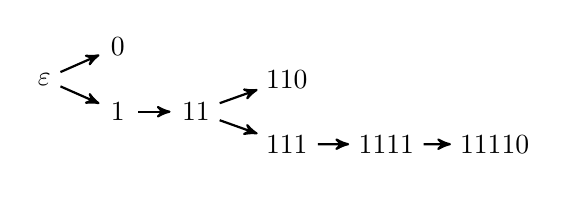
\begin{tikzpicture}[->,>=stealth',auto,thick, scale = 0.55,state/.style={circle,inner sep=2pt}]
	\node [state] at (-0.2,0) (r) {$\varepsilon$};
	\node [state] at (1.5,0.75) (n0) {$0$};
	\node [state] at (1.5,-0.75) (n1) {$1$};
	\node [state] at (3.3,-0.75) (n11) {$11$};
	\node [state] at (5.4,0) (n110) {$110$};
	\node [state] at (5.4,-1.5) (n111) {$111$};
	\node [state] at (7.7,-1.5) (n1111) {$1111$};
	\node [state] at (10.2,-1.5) (n11110) {$11110$};
	
	\path[->]
	(r) edge (n1)
	(r) edge (n0)
	(n1) edge (n11)
	(n11) edge (n110)
	(n11) edge (n111)
	(n111) edge (n1111)
	(n1111) edge (n11110);  	
\end{tikzpicture} 
\end{center}
In this case, we have that $q = \{\varepsilon, 0, 1, 11, 110, 111, 1111, 11110\}$, so $q$ is a finite and prefix-closed subset of $\bB = \{0,1\}^*$. The owner of each block $b \in q \smallsetminus \{ \varepsilon\}$ is given by the  the last symbol of $b$; for instance, we have that $\owner(11) = 1$ and $\owner(11110) = 0$. Moreover, the longest path in $q$ is $\pi = \{\varepsilon, 1, 11, 111, 1111, 11110\}$, so that the blockchain of $q$ is $\pi$ (in symbols, $\bchain(q) = \pi$). 
%Thus, we have that the blocks that belong to the blockchain of $q$ are $\varepsilon$, $1$, $11$, $111$, $1111$, $11110$, since these are precisely the blocks in $q$ in the path from $\varepsilon$ to $11110$ (in symbols, $\epath(\bchain(q)) = \{\varepsilon, 1, 11, 111, 1111, 11110\}$). Notice that the information about these blocks is important as the reward of each player depends on the blocks that belong to her in the blockchain. For instance, if the reward for each block is a constant $c$, then we have that the reward of player 1 is $4 c$ in $q$, as four blocks in the blockchain of $q$ belong to this player. 
Finally, notice that $|q| = 8$, as $q$ is a set consisting of eight blocks.

	Assume now that $q'$ is the following state of the game:
	\begin{center}
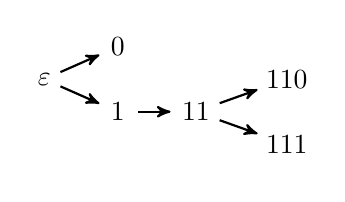
\begin{tikzpicture}[->,>=stealth',auto,thick, scale = 0.55,state/.style={circle,inner sep=2pt}]
	\node [state] at (-0.2,0) (r) {$\varepsilon$};
	\node [state] at (1.5,0.75) (n0) {$0$};
	\node [state] at (1.5,-0.75) (n1) {$1$};
	\node [state] at (3.3,-0.75) (n11) {$11$};
	\node [state] at (5.4,0) (n110) {$110$};
	\node [state] at (5.4,-1.5) (n111) {$111$};

	\path[->]
	(r) edge (n1)
	(r) edge (n0)
	(n1) edge (n11)
	(n11) edge (n110)
	(n11) edge (n111);
\end{tikzpicture} 
\end{center}
In this case, we have that $\bchain(q')$ is not defined since the paths $\pi_1 = \{\varepsilon, 1, 11, 110\}$ and $\pi_2 = \{\varepsilon, 1, 11, 111\}$ are tied for the longest path in $q'$. \qed
\end{example}


Real-life bitcoin blocks also contain transactions that indicate movement of money in the system, and thus there are 
several different blocks that a player $p$ can use to extend the current state when mining upon a block $b$ (e.g, depending  on the ordering of transactions, or the nonce being used to announce the block). Since we are interested primarily in miners behaviour, we just focus on the owner of the block following $b$, and do not consider the possibility of two different blocks belonging to $p$ being added on top of $b$. Alternatively, if we consider the Bitcoin protocol, we could say that all the different blocks that $p$ can put on top of $b$ are considered as~equivalent. 
%\juan{moving this to the reward section}
%\etienne{We may have to specify that it is under the assumption that there are no fees or that they are negligible.} \marcelo{Etienne is right about this, depending on the transactions included in the block the reward could be different. I don't think we should talk about reward here.}

\subsection{Actions of a miner}
On each step, miners looking to maximize their rewards choose a block in the current state, and attempt to mine on top of this block. Thus, in each turn, each of the players race to place the next block in the state, and only one of them succeeds. The probability of succeeding is directly related to the comparative amount of hash power available to this player, the more hash power the likely it is that she will mine the next block before the rest of the players. Once a player places a block, this block is added to the current state, obtaining a different state from which the game continues.

Let $p \in \bP$. Given a block $b \in \bB$ and a state $q \in \bQ$, we denote by $\mine(p,b,q)$ an action played in the mining game in which player $p$ mines on top of block $b$. Such an action $\mine(p,b,q)$ is considered to be valid if $b \in q$ and $b\cdot p \not\in q$. The set of valid actions for player $p$ is collected in the set:
\begin{multline*}
\bA_p \ = \ \{ \mine(p,b,q) \mid b \in \bB, q \in \bQ \text{ and}\\\mine(p,b,q) \text{ is a valid action}\}.
\end{multline*}
Moreover, given $a \in \bA_p$ with $a = \mine(p,b,q)$, the result of applying $a$ to $q$, denoted by $a(q)$, is defined as the state $q \cup \{b \cdot p\}$. Finally, we denote by $\bA$ the set of combined actions for the $m$ players, that is, $\bA = \bA_0 \times \bA_1 \times \cdots \times \bA_{m-1}$.

\subsection{The pay-off of a miner}
The Bitcoin protocol give reward to the owner of a block if it is part of the blockchain and has been confirmed by 100 blocks. A payment function which closely follows this protocol has been introduced in \cite{}, however it adds the constraint that for every level of the state's tree only one block give a reward (the first one which has been confirmed by 100 blocks). Due to this constraint if a fork longer than 100 blocks would happen, some blocks belonging to the new blockchain won't give any reward to their owners (which contradicts the bitcoin's rules). As a matter of fact the model nullify the incentive of performing a fork longer than 100 \cite{}. One could argue that a fork longer than 100 would destroy the market confidence and therefore can be ignored. It might be the case with the current state of crypto-currencies, but as the technology become more widely adopted (government or bank), such argument can not be use any-more.

In stochastic game, the pay-off of a player $p \in \bP$, is given by a function $r_p: \bQ \times \bA \mapsto \mathbb{R}$, and the payoff function of the game is $\bR = (r_0, r_1, \ldots, r_{m-1})$.
As the pay-off of a player is determined by the state and not the history of states, a function which rewards players once and only once for each block they own in the blockchain, can not be build (see example \ref{eximpo}). We propose a model where on every states, we pay miners a constant $c$ for each of the blocks they already have in the blockchain, plus the new block they will potentially mine. This model puts a strong incentive in maintaining blocks in the blockchain and does not nullify the incentive to fork.
The main concern regarding this pay-off model, is that we might end-up giving reward to player multiple times for the same block (once for each state where the block belongs to the blockchain). In the following sections we address this specific matter \ref{} and formally defines our pay-off functions \ref{}. 

Note that if in the general case a pay-off is a function from $\bQ \times \bA$ to $\mathbb{R}$, in our model the pay-off for a player $p$ does not depend on the action of other players. Hence we can extend the definition such that for any state $q$ and any player $p$ we have $r_p(q) = r_p(q',(\ba,a_p))$ with $q' = q \setminus b$ a state and $a_p = mine(p,b,q')$ a valid action.  
 
 
\subsection{The definition of the game}
As a last component of the game, we assume that $\pr : \bQ \times \bA \times \bQ \to [0,1]$ is a transition probability function satisfying that for every state $q \in \bQ$ and combined action $\ba = (a_0, a_1, \ldots, a_{m-1})$ in $\bA$:
\begin{eqnarray*}\label{eq-prop}
\sum_{p=0}^{m-1} \pr(q, \ba, a_p(q)) & = & 1.
\end{eqnarray*}
Notice that if $p_1$ and $p_2$ are two different players, then for every action $a_1 \in \bA_{p_1}$, every action $a_2 \in \bA_{p_2}$ and every state $q \in \bQ$, it holds that $a_1(q) \neq a_2(q)$. Thus, we can think of $\pr(q, \ba, a_p(q))$ as the probability that player $p$ places the next block, which will generate the state $a_p(q)$. 

Summing up, from now on we consider an infinite stochastic game $\Gamma = (\bP,\bA,\bQ,\bR,\pr)$, where $\bP$ is the set of players, $\bA$ is the set of combined actions, $\bQ$ is the set of states, $\bR$ is the pay-off function and $\pr$ is the transition probability function.
%\begin{itemize}
%	\item $\bP$ is the set of players.
%	\item $\bA$ is the set of possible actions.
%	\item $\bQ$ is the set of states.
%	\item $\bR$ is the pay-off function.
%	\item $\pr$ is the transition probability function.
%\end{itemize} 

\subsubsection{Games with constant hash power}
%\label{sec-simp}
Recall that the probability that action $a_p$ is indeed executed is given by $\pr(q, \ba, a_p(q))$. As we have mentioned, such a probability is directly related with the hash power of player $p$, the more hash power the likely it is that action $a_p$ is executed and $p$ mines the next block before the rest of the players. In what follows, we assume that the hash power of each player does not change during the mining game, which is captured by the following condition:
\begin{itemize}
\item For every $q, q' \in \bQ$, every $\ba, \ba' \in \bA$ such that $\ba = (a_0, a_1$, $\ldots$, $a_{m-1})$ and $\ba' = (a'_0, a'_1, \ldots, a'_{m-1})$,  and every player $p \in \bP$, it holds that $\pr(q, \ba, a_p(q)) = \pr(q', \ba', a'_p(q'))$.
\end{itemize}
Thus, we assume from now on that this condition is satisfied. In particular, for each player $p \in \bP$, we assume that that 
$\pr(q, \ba, a_p(q)) = h_p$ for every $q \in \bQ$ and $\ba \in \bA$ with $\ba = (a_0, a_1, \ldots, a_{m-1})$, and we refer to $h_p$ as the hash power of player $p$. 
%Moreover, we define $\bH = (h_0, h_1, \ldots, h_{m-1})$ as the hash power distribution, and we replace $\pr$ by $\bH$ in the definition of an an infinite stochastic game, so that $\Gamma = (\bP,\bA,\bQ,\bR,\bH)$. 
Moreover, we assume that $h_p > 0$ for every player $p \in \bP$, as if this not the case then $p$ can just be removed from the mining game. 

\subsection{Utility and equilibria of the game}
We have defined a game that can capture miners' interactions. A fundamental component of such a game is the strategy that each player decides to take, which combined determine the utility of each player. In particular, miners take actions and decide about strategies trying to maximize their utility. In this sense, a stationary equilibrium of the game is a fundamental piece of information about miners' behavior, as such an equilibrium is a combination of players' strategies where no miner has an incentive to perform a different action. The notions of strategy, utility and stationary equilibrium are the last components of our game-theoretical characterization of mining in Bitcoin, and they are defined in this section.

A strategy for a player $p \in \bP$ is a function $s : \bQ \rightarrow \bA_p$. 
We define $\bS_p$ as the set of all strategies for player $p$, and $\bS = \bS_0 \times \bS_{1} \times \cdots \times \bS_{m-1}$ as the set of combined strategies for the game (recall that we are assuming that $\bP = \{0, 1, \ldots, m-1\}$ is the set of players). 

As usual, we are interested in understanding which strategies fare better than others, which we capture by the notions of  utility and equilibrium. To define these, we need some additional notation. 
Let $\bs = (s_0, s_1, \ldots, s_{m-1})$ be a strategy in $\bS$. Then given $q \in \bQ$, define $\bs(q)$ as the combined action $(s_0(q), s_1(q), \ldots, s_{m-1}(q))$. Moreover, given an initial state $q_0 \in \bQ$, 
the probability of reaching state $q \in \bQ$, denoted by $\pr^{\bs}(q \mid q_0)$, is defined as 0 if $q_0 \not\subseteq q$, and otherwise it is recursively defined as follows: if $q =  q_0$, then $\pr^{\bs}(q \mid q_0) = 1$; otherwise, we have that $|q| - |q_0| = k$, with $k \geq 1$, and
$$
\pr^{\bs}(q \mid q_0) =
\sum_{\substack{q' \in \bQ \,:\\ q_0 \subseteq q' \text{ and } |q'| - |q_0| = k-1}}
 \pr^{\bs}(q' \mid q_0) \cdot \pr(q', \bs(q'), q).
 $$
In this definition, if for a player $p$ we have that $s_p(q') = a$ and $a(q') = q$, then $\pr(q', \bs(q'), q) = h_p$. Otherwise, we have that $\pr(q', \bs(q'), q) = 0$. 
%Hence, consistently with the simplification described before, we can replace the transition probability function $\pr$ by the hash power distribution $\bH$ when computing $\pr^{\bs}(q \mid q_0)$. 
It should be noticed that the framework just described corresponds to a Markov chain; in particular, the probability of reaching a state from an initial state is defined in the standard way for Markov chains~\cite{MU05}. However, we are not interested in the steady distribution for such a Markov chain and, thus, we do not explore more this connection in this paper.

We finally have all the necessary ingredients to define the utility of a player in a mining game given a particular strategy. As is common 
when looking at personal utilities, we define it as the summation of the expected rewards, and choose 
to impose a discount for future rewards using a factor $\beta \in (0,1)$. 

\begin{mydef}
\label{def-utility}
The $\beta$--discounted utility of player $p$ for the strategy $\bs$ from the state $q_0$ in 
the mining game, denoted by $u_p(\bs \mid q_0)$, is defined as:
\begin{eqnarray*}
u_p(\bs \mid q_0) & = & (1 - \beta) \cdot  \sum_{q \in \bQ \,:\, q_0 \subseteq q} \beta^{|q|-|q_0|} \cdot  r_p(q) \cdot \pr^{\bs}(q \mid q_0).
\end{eqnarray*}
\end{mydef}
Notice that the value $u_p(\bs \mid q_0)$ may not be defined if the series $\sum_{q \in \bQ \,:\, q_0 \subseteq q} \beta^{|q|-|q_0|} \cdot  r_p(q) \cdot \pr^{\bs}(q \mid q_0)$ diverges. To avoid this problem, from now on we assume that for every pay-off function $\bR = (r_0, \ldots, r_{m-1})$, there exists a polynomial $P$ such that $|r_p(q)| \leq P(|q|)$ for every player $p \in \bP$ and state $q \in \bQ$. Under this simple yet general condition, it is posible to prove that $u_p(\bs \mid q_0)$ is a real number (see Appendix \ref{sec-conver} for a proof of this property). 

As a last ingredient in our formalization, we need to introduce the notion stationary equilibrium.
Given a player $p \in \bP$, a combined strategy $\bs \in \bS$, with $\bs = (s_0,s_1, \ldots, s_{m-1})$, and a strategy $s$ for player $p$ ($s \in \bS_p$), we denote by $(\bs_{-p}, s)$ the strategy $(s_0, s_1, \ldots s_{p-1},s,s_{p+1}, \ldots, s_{m-1})$.
\begin{mydef}
A strategy $\bs$ is a $\beta$--discounted stationary equilibrium from the state $q_0$ in  the %infinite 
mining game if for every player $p \in \bP$ and every strategy $s$ for player $p$ $(s \in\bS_p)$, it holds that:
\begin{eqnarray*}u_p(\bs \mid q_0)  & \geq  & u_p ((\bs_{-p},s) \mid q_0).
\end{eqnarray*}
\end{mydef}
We conclude this section by going deeper into the definition of utility, given the key role it plays in our framework. 
Definition~\ref{def-utility} corresponds to the usual notion of average discounted utility \marcelo{A citation is needed here}. In particular, if the starting point of the game is a state $q_0$, then for every state $q$ such that $q_0 \subseteq q$, the pay-off of a player $p$ in $q$ is $\beta^{|q|-|q_0|} \cdot r_p(q)$, where $|q|-|q_0|$ is the number of steps that have to be performed to reach $q$ from $q_0$ so the discount factor $\beta^{|q|-|q_0|}$ has to be applied. The uncertainty  about reaching state $q$ from $q_0$ is taking into consideration by including the term $\pr^{\bs}(q \mid q_0)$, which tell us that the expected payoff for the state $q$ is $\beta^{|q|-|q_0|} \cdot  r_p(q) \cdot \pr^{\bs}(q \mid q_0)$.  
%
As a last comment on the definition of utility, notice that a block $b$ can be included in an infinite number of states $q$ such that $\pr^{\bs}(q \mid q_0) > 0$. But the reward obtained by a player $p$ for this block $b$ should not be added more than once, which is the reason to include the term $(1 - \beta)$ in the definition of utility. Let us formalize this claim in more precise terms. 

Assume that the reward obtained by a player $p$ for a block $b$ in a state $q$ is given by $r_p(b,q)$, so that $r_p(q) = \sum_{b \in q} r_p(b,q)$. Notice that such decomposition can always be done; in fact, it can be done in a natural and straightforward way for the pay-off functions considered in this paper and in other game-theoretical formalizations of Bitcoin mining \cite{mininggames:2016}. Then we have that:
\begin{align*}
u_p(\bs \mid \{\varepsilon\}) & =  (1 - \beta) \cdot  \sum_{q \in \bQ} \beta^{|q|-|\{\varepsilon\}|} \cdot  r_p(q) \cdot \pr^{\bs}(q \mid \{\varepsilon\})\\
& =  (1 - \beta) \cdot \sum_{q \in \bQ} \beta^{|q|-1} \cdot  \bigg(\sum_{b \in q} r_p(b,q) \bigg) \cdot \pr^{\bs}(q \mid \{\varepsilon\})\\
& = (1 - \beta) \cdot \sum_{b \in \bB} \sum_{q \in \bQ \,:\, b \in q} \beta^{|q|-1} \cdot r_p(b,q) \cdot \pr^{\bs}(q \mid \{\varepsilon\}).
\end{align*}
For the sake of readability, we assume that the game is starting from the initial state $\{\varepsilon\}$ that consists only of the genesis block. Notice that $|\{\varepsilon\}| = 1$, so that the discount factor for a state $q$ is $\beta^{|q|-1}$. Now assume that there is a maximum value for the reward of a block $b$ for player $p$, which is denoted by $M_p(b)$. Thus, we have that there exists $q_1 \in \bQ$ such that $b \in q_1$ and $M_p(b) = r_p(b,q_1)$, and for every $q_2 \in \bQ$ such that $b \in q_2$, it holds that $r_p(b,q_2) \leq M_p(b)$. Again, such an assumption is satisfied by the pay-off functions considered in this paper and in other game-theoretical formalizations of Bitcoin mining \cite{mininggames:2016}. Then we have that:
\begin{align*}
&\sum_{b \in \bB} \sum_{q \in \bQ \,:\, b \in q} \beta^{|q|-1} \cdot r_p(b,q) \cdot \pr^{\bs}(q \mid \{\varepsilon\})
\ \leq \\  
&\hspace{40pt}  \sum_{b \in \bB} \sum_{q \in \bQ \,:\, b \in q} \beta^{|q|-1} \cdot M_p(b) \cdot \pr^{\bs}(q \mid \{\varepsilon\}) \ =\\
&\hspace{40pt}  \sum_{b \in \bB} M_p(b) \cdot\bigg(\sum_{q \in \bQ \,:\, b \in q} \beta^{|q|-1}  \cdot \pr^{\bs}(q \mid \{\varepsilon\})\bigg) \ \leq\\
&\hspace{40pt}  \sum_{b \in \bB} M_p(b) \cdot\bigg(\sum_{q \in \bQ \,:\, |q| \geq |b|+1} \beta^{|q|-1}  \cdot \pr^{\bs}(q \mid \{\varepsilon\})\bigg) \ = \\
&\hspace{40pt}  \sum_{b \in \bB} M_p(b) \cdot\bigg(\sum_{i=|b|+1}^\infty \sum_{q \in \bQ \,:\, |q| = i} \beta^{|q|-1}  \cdot \pr^{\bs}(q \mid \{\varepsilon\})\bigg) \ = \\
&\hspace{40pt}  \sum_{b \in \bB} M_p(b) \cdot\bigg(\sum_{i=|b|+1}^\infty \beta^{i-1} \cdot \sum_{q \in \bQ \,:\, |q| = i} \pr^{\bs}(q \mid \{\varepsilon\})\bigg).
\end{align*}
By the definition of the transition probability function $\pr^{\bs}$, it is straightforward to prove that $\sum_{q \in \bQ \,:\, |q| = i} \pr^{\bs}(q \mid \{\varepsilon\}) = 1$. Hence, we conclude that:
\begin{align*}
&\sum_{b \in \bB} M_p(b) \cdot\bigg(\sum_{i=|b|+1}^\infty \beta^{i-1} \cdot \sum_{q \in \bQ \,:\, |q| = i} \pr^{\bs}(q \mid \{\varepsilon\})\bigg) \ = \\
&\hspace{60pt}  \sum_{b \in \bB} M_p(b) \cdot\bigg(\sum_{i=|b|+1}^\infty \beta^{i-1}\bigg) \ = \\
&\hspace{60pt}  \sum_{b \in \bB} M_p(b) \cdot \beta^{|b|} \cdot \bigg(\sum_{j=0}^\infty \beta^{j}\bigg) \ = \\
&\hspace{60pt}  \sum_{b \in \bB} M_p(b) \cdot \beta^{|b|} \cdot \frac{1}{1-\beta},
\end{align*}
where $|b|$ is the length of block $b$ considered as a string. Therefore, we finally conclude that:
\begin{eqnarray*}
u_p(\bs \mid \{\varepsilon\}) & \leq &  \sum_{b \in \bB} \beta^{|b|} \cdot M_p(b).
\end{eqnarray*}
Thus, the pay-off obtained by player $p$ for a block $b$ is at most $\beta^{|b|} \cdot M_p(b)$, that is, the maximum reward that she can obtained for the block $b$ in a state multiplied by the discount factor $\beta^{|b|}$, where $|b|$ is the minimum number of steps that have to be performed to reach a state containing $b$ from the initial state $\{\varepsilon\}$.

\marcelo{The justification of the utility function is long, we can move the proof to the appendix and only keep the bound $u_p(\bs \mid \{\varepsilon\}) \leq \sum_{b \in \bB} \beta^{|b|} \cdot M_p(b)$.}

%Along the paper we will also consider games ending in a finite number of steps. For these games we redefine the notion of $\beta$-discounted utilities by summing up the rewards only up to $n$, and define the notion of a $\beta$-discounted equilibrium accordingly. 
%\marcelo{We are not going to consider games ending in a finite number of steps in this paper, right?}

%\marcelo{In these definitions we are assuming that $u_p(\bs \mid q_0)$ is defined, which could not be the case if the series diverges. We should say something about this.}
%\francisco{True. Something like ``$r$ is a decreasing function and card$(Q)$ is controlled by $p^{|q|}$'' (worst case scenario, every player forks), so we should be OK.}

\iffalse

\subsection{Pay-off of a miner (extended version)}


\etienne{I still have to work on the actual wording, but i think it will look like that. I choosed to push the graph in appendix for space reasons, what do u think ?}

In stochastic game,the pay-off of a player $p \in \bP$, is given by a function $r_p: \bQ \times \bA \mapsto \mathbb{R}$, and the payoff function of the game is $\bR = (r_0, r_1, \ldots, r_{m-1})$.
But how should the function $r_p(q,\ba)$ look like? Recall that one of the rules of bitcoin is that the money can only 
be spent when it is given in blocks that are part of the blockchain. Thus, the first idea that comes into mind is to 
reward players every time they put a block in the blockchain. However, this is not a good function, as it is not possible to build a pay-off function which rewards them once and only once for each block in the blockchain (see example \ref{eximpo}).

\begin{myex} 
\label{eximpo}
\begin{figure}
\begin{center}
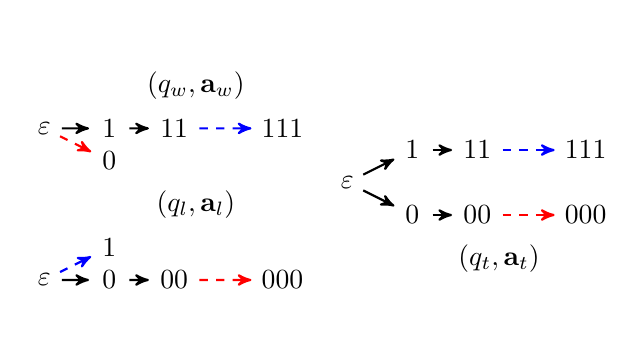
\begin{tikzpicture}[->,>=stealth',auto,thick, scale = 0.55,state/.style={circle,inner sep=2pt}]

    % The graph A
    \node [state] at (3.5,2.25) (name1) {$(q_w,\ba_w)$};
	\node [state] at (0,1.25) (Ra0) {$\varepsilon$};
	\node [state] at (1.5,0.5) (0a0) {$0$};
	\node [state] at (1.5,1.25) (1a0) {$1$};
	\node [state] at (3,1.25) (11a0) {$11$};
	\node [state] at (5.5,1.25) (111a0) {$111$};
	
	 % The graph A
	\node [state] at (0,-2.25) (Ra1) {$\varepsilon$};
	\node [state] at (1.5,-1.5) (0a1) {$1$};
	\node [state] at (1.5,-2.25) (1a1) {$0$};
	\node [state] at (3,-2.25) (11a1) {$00$};
	\node [state] at (5.5,-2.25) (111a1) {$000$};
	\node [state] at (3.5,-0.5) (name2) {$(q_l,\ba_l)$};
	
	% The graph A
	\node [state] at (7,0) (Ra) {$\varepsilon$};
	\node [state] at (8.5,0.75) (1a) {$1$};
	\node [state] at (8.5,-0.75) (0a) {$0$};
	\node [state] at (10,0.75) (11a) {$11$};
	\node [state] at (10,-0.75) (00a) {$00$};
	\node [state] at (12.5,0.75) (111a) {$111$};
	\node [state] at (12.5,-0.75) (000a) {$000$};
	\node [state] at (10.5,-1.75) (name3) {$(q_t,\ba_t)$};	
	
	% Graph edges
	\path[->]
	(Ra) edge (1a)
	(Ra) edge (0a)
	(1a) edge (11a)
	(0a) edge (00a)
	(Ra1) edge (1a1)
	(1a1) edge (11a1)
	(Ra0) edge (1a0)
	(1a0) edge (11a0)
	;  	
	
	% Graph edges
	\path[dashed,blue]
	(Ra1) edge (0a1)
	(11a) edge (111a)
	(11a0) edge (111a0)
	;  	
	
	\path[dashed,red]
	(Ra0) edge (0a0)
	(00a) edge (000a)
	(11a1) edge (111a1)
	;


\end{tikzpicture} 
\end{center}
\caption{An example showing that I should want to try to compete when some other player forks on my blocks. \label{fig-impo}}
\end{figure}



Consider a pay-off function $r_1$ for player $1$, it is immediate to understand that in the situation described by $q_l$ the value $r_1(q_l,\ba_l)$ should be $0$, indeed player $1$ did not put any new block in the blockchain. While in the situation described in $q_w$, $r_1(q_w,\ba_w)$ should reward the player $1$ for his block $111$.
\\Now consider the tie situation described in $q_t$. What should be the value of $r_1(q_t,\ba_t)$? Either $r_1(q_t,\ba_t)$ only rewards player 1 for his block $111$, and if $q_t$ has been reach through $q_l$ then he would never has been paid for the block $1$. Or $r_1(q_t,\ba_t)$ rewards player 1 for every blocks involved in the tie and if $q_t$ is reach trough $q_w$, he would have been paid twice for the blocks $1$ and $11$. The pay-off not relying on the history of states, cannot distinguish those two situations hence it is not possible to build a pay-off function which pay once and only once the player for each block in the blockchain.

\end{myex} 

Ideally, one would like to reward players according to the blocks they have in the blockchain when the game terminates (or the limit of that number, in the case of infinite games). The problem is that we cannot really know what this pay-off will be until the game is actually finished, and thus we cannot model this pay-off in our stochastic game setting. 
What we do instead is to use a heuristic for this reward called cumulative pay-off model and denoted $r_p^c(.)$. On each turn, we pay miners a constant $c$ for each of the blocks they already have in the blockchain, plus the new block they have potentially mining them. This clearly puts a strong incentive in maintaining blocks, but also on mining new blocks on the blockchain. 
\\Note that in the general case a pay-off is a function from $\bQ \times \bA$ to $\mathbb{R}$, in our model the pay-off of player $p$ does not depend on the action of other players. Hence we extend the definition of the cumulative pay-off function such that for any state $q$ and any player $p$ we have $r_p^c(q) = r_p^c(q',(\ba,a_p))$ with $q' = q \setminus b$ and $a_p = mine(p,b,q')$. We also consider a function where the reward for each new block in the blockchain decreases by a constant factor $\alpha$. We will formally define our cumulative payoff functions in the following sections. 


The main concern regarding this pay-off function called cumulative pay-off, is that the early blocks may have a lot more value than the later ones (not because of a decreasing reward, but because early blocks are counted multiple times).
In order to show that this problem is not as strong as it might seems, we compared the sum of the rewards obtained under the cumulative, relative \cite{} and absolute \cite{} pay-off models on pseudo-randomly generated  blockchains. We considere a fix number of blocks distrubuted upon players $\bP$ and we assume they always mined upon the blockchain (default behaviour). Therefore the only variable between two iterations is the position of the blocks own by each players. The total number of blocks at the end of each iteration is 100.000 and we have done 1000 iterations. Let $i \in \{1\cdots 1000\}$, we denote by $q_i$ the final state of the iteration. For any state $q \subseteq q_i$ and any player $p \in \bP$ we denote $r_p^a(q)$ resp. $r_p^r(q)$ the absolute resp. relative pay-off function. We have that $r_p^a(q) = c$ if $owner(bc(q)) = p$ and $r_p^a(q) = 0$ otherwise. And that $r_p^r(q) = \frac{c}{|q|}$ if $owner(bc(q)) = p$ and $r_p^r(q) = 0$ otherwise. Finally with $$R_p^x(q_i) = \frac{\sum\limits_{q \subseteq q_i} r_p^x(q)}{\sum\limits_{p' \in \bP}\sum\limits_{q \subseteq q_i} r_{p'}^x(q)} $$ we call maximum difference the value:\\ $\underset{p \in \bP}{max}\left(\underset{{i \in \{1 \cdots 10
00\}}}{max}(R_p^x(q_i)) - \underset{{i \in \{1 \cdots 10
00\}}}{min}(R_p^x(q_i))\right)$\\and average difference the value: $\underset{{i,i' \in \{1 \cdots 10
00\}}}{average}(|R_p^x(q_i) - R_p^x(q_{i'})|) $.

\begin{figure}
\begin{tabular}{c|c|c|}
. & maxium difference & average difference   \\
\hline
constant pay-off & 0 & 0 \\
\hline
relative pay-off & x.x &  x.x \\
\hline
cumulative pay-off &  x.x &  x.x \\
\end{tabular}
\caption{Results of the simulation for absolute, relative and cumulative models}
\end{figure}

As you can see in the table \ref{}, the cumulative model yields to a behaviour inbetween the constant and relative models. Therefore, even if the value for the early blocks of the blockchain is higher than the value for the later ones, the difference between them is reasonable. More details and results about this experimentation are available in appendix \ref{}.

An other possible pay-off function presented in \cite{}, introduced a delay $d$ before rewarding a player for a block. Moreover this pay-off also insure that only one block for each depth is going to receive a payment (the first one for which the delay $d$ is achieve). It is really close to the bitcoin protocol as miners have to wait 100 blocks in order to use their coin-base transaction bitcoins, however the constraint that only one block per depth can be paid nullify the incentive of performing a fork longer than $d$. One could argue that a fork longer than $d$ would destroy the market confidence hence the value and therefore can be ignored. It might be the case with the current state of crypto-currencies, but if the technology become more widely adopted (government or bank), such argument can not be use any-more.



%The other issue is what to do when the blockchain is contested, and there are at least two paths sharing the maximal length. A simple solution 
%would be to declare that players receive no pay-off when this happens. But again, this would lead to strange behaviours in which players with several blocks buried deep in the blockchain would receive no reward for this blocks because of a contest in the newer parts of the blockchain. 
%In order to avoid this scenario, we choose to maintain the reward for blocks buried deep in the blockchain even when there is a contest, 
%and formalise this as follows. 
\fi

\iffalse

\begin{myex} 
\label{eximpo}
\begin{figure}
\begin{center}
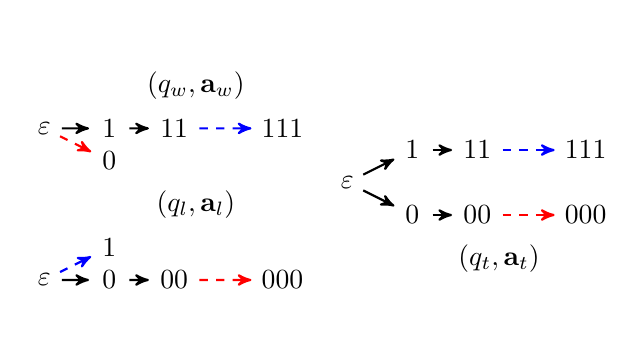
\begin{tikzpicture}[->,>=stealth',auto,thick, scale = 0.55,state/.style={circle,inner sep=2pt}]

    % The graph A
    \node [state] at (3.5,2.25) (name1) {$(q_w,\ba_w)$};
	\node [state] at (0,1.25) (Ra0) {$\varepsilon$};
	\node [state] at (1.5,0.5) (0a0) {$0$};
	\node [state] at (1.5,1.25) (1a0) {$1$};
	\node [state] at (3,1.25) (11a0) {$11$};
	\node [state] at (5.5,1.25) (111a0) {$111$};
	
	 % The graph A
	\node [state] at (0,-2.25) (Ra1) {$\varepsilon$};
	\node [state] at (1.5,-1.5) (0a1) {$1$};
	\node [state] at (1.5,-2.25) (1a1) {$0$};
	\node [state] at (3,-2.25) (11a1) {$00$};
	\node [state] at (5.5,-2.25) (111a1) {$000$};
	\node [state] at (3.5,-0.5) (name2) {$(q_l,\ba_l)$};
	
	% The graph A
	\node [state] at (7,0) (Ra) {$\varepsilon$};
	\node [state] at (8.5,0.75) (1a) {$1$};
	\node [state] at (8.5,-0.75) (0a) {$0$};
	\node [state] at (10,0.75) (11a) {$11$};
	\node [state] at (10,-0.75) (00a) {$00$};
	\node [state] at (12.5,0.75) (111a) {$111$};
	\node [state] at (12.5,-0.75) (000a) {$000$};
	\node [state] at (10.5,-1.75) (name3) {$(q_t,\ba_t)$};	
	
	% Graph edges
	\path[->]
	(Ra) edge (1a)
	(Ra) edge (0a)
	(1a) edge (11a)
	(0a) edge (00a)
	(Ra1) edge (1a1)
	(1a1) edge (11a1)
	(Ra0) edge (1a0)
	(1a0) edge (11a0)
	;  	
	
	% Graph edges
	\path[dashed,blue]
	(Ra1) edge (0a1)
	(11a) edge (111a)
	(11a0) edge (111a0)
	;  	
	
	\path[dashed,red]
	(Ra0) edge (0a0)
	(00a) edge (000a)
	(11a1) edge (111a1)
	;


\end{tikzpicture} 
\end{center}
\caption{An example showing that I should want to try to compete when some other player forks on my blocks. \label{fig-impo}}
\end{figure}

Consider a pay-off function $r_1$ for player $1$, it is immediate to understand that in the situation described by $q_l$ the value $r_1(q_l,\ba_l)$ should be $0$, indeed player $1$ did not put any new block in the blockchain. While in the situation described in $q_w$, $r_1(q_w,\ba_w)$ should reward the player $1$ for his block $111$.
\\Now consider the tie situation described in $q_t$. What should be the value of $r_1(q_t,\ba_t)$? Either $r_1(q_t,\ba_t)$ only rewards player 1 for his block $111$, and if $q_t$ has been reach through $q_l$ then he would never has been paid for the block $1$. Or $r_1(q_t,\ba_t)$ rewards player 1 for every blocks involved in the tie and if $q_t$ is reach trough $q_w$, he would have been paid twice for the blocks $1$ and $11$. The pay-off not relying on the history of states, cannot distinguish those two situations hence it is not possible to build a pay-off function which pay once and only once the player for each block in the blockchain.

\end{myex} 
\fi




	%!TEX root = main.tex

\section{A Game-theoretic Formalization of Bitcoin Mining}
\label{sec-formalization}

The mining game is played by a set $\bP = \{0, 1, , \ldots, m-1\}$ of players, with $m \geq 2$.
In this game, each player has some reward depending on the number of blocks she owns. Every block must point to a previous block, except for the first block which is called the {\em genesis block}. Thus, the game defines a tree of blocks. Each block is put by one player, called the {\em owner} of this block. Each such tree is called a {\em state of the game}, or just {\em state}, and it represents the knowledge that each player has about the blocks that have been mined thus far.

The key question for each player is, then, where do I put my next block? In bitcoin, miners are only allowed to spend their reward as long
as their blocks belongs to the \emph{blockchain} of a state, which is simply the longest chain of blocks in this state. Thus, players face essentially two possibilities: they can put their blocks right after the end of the longest chain (the blockchain), or they can try to \emph{fork}
from the longest chain, betting that a smaller chain will eventually become the blockchain. As the likelihood of
mining the next block is directly related to the comparative hash power of a player, it makes sense to model this game as an infinite
stochastic game, in which the probability of executing the action of a player $p$ is given by her comparative hash power.

In what follows, we first define the components of the infinite stochastic games considered in this paper, and the notions of strategy, utility  and equilibrium for such games. Our formalization is similar to others presented in the literature \cite{mininggames:2016}, except for the way in which miners are rewarded and the way in which these rewards are accumulated in the utility function. Hence, we analyse them in more detailed in Section \ref{sec-pay-ut}, emphasizing the properties of these two elements that are fundamental for our formalization.

% Let us now turn to the formal definition of the game.

\subsection{The definition of the game}
\subsubsection{Blocks, states and the notion of blockchain}\label{sub:states}

In a game played by $m$ players, a block is defined a string $b$ over the alphabet $\{0,1,\ldots$, $m-1\}$. We denote by $\bB$ the set of all blocks, that is, $\bB = \{0,1,\ldots , m-1\}^*$. Each block apart from $\varepsilon$ has a unique owner, defined by the function $\owner: (\bB \smallsetminus \{\varepsilon\}) \rightarrow \{0,1, \ldots ,m-1\}$ such that $\owner(b)$ is equal to the last symbol of $b$. As in \cite{mininggames:2016}, a state of the game is defined as a tree of blocks. More precisely, a state of the game, or just state,  is a finite and nonempty set of blocks $q \subseteq \bB$ that is prefix closed. That is, $q$ is a set of strings over the alphabet $\{0,1,\ldots, m-1\}$ such that if $b\in q$, then every prefix of $b$ (including the empty word $\varepsilon$) also belongs to $q$. Note that a prefix closed subset of $\bB$ uniquely defines a tree with $\varepsilon$ as the root.
%
The intuition here is that each element of $q$ corresponds to a block that was put into the state $q$ by some player. The genesis block corresponds to $\varepsilon$. When a player $p$ decides to mine on top of a block $b$, she puts another block into the state defined by the string $b\cdot p$, where we use notation $b_1 \cdot b_2$ for the concatenation of two strings $b_1$ and $b_2$.
%
Notice that with this terminology, given $b_1, b_2 \in q$, we have that $b_2$ is a descendant of $b_1$ in $q$ if $b_1$ is a prefix of $b_2$, which is denoted by $b_1 \preceq b_2$. Moreover, a path in $q$ is a nonempty set $\pi$ of blocks from $q$ for which there exist blocks $b_1, b_2$ such that $\pi = \{ b \mid b_1 \preceq b$ and $b \preceq b_2\}$; in particular, $b_2$ is a descendant of $b_1$ and $\pi$ is said to be a path from $b_1$ to $b_2$.
Finally, let $\bQ$ be the set of all possible states in a game played by $m$ players, and for a state $q \in \bQ$, let $|q|$ be its size, measured as the cardinality of the set $q$ of strings (or blocks).

Given a state $q$, we say that the {\em blockchain} of $q$ is the path $\pi$ in $q$ of the biggest length, in the case that this path is unique, in which case we denote it by $\bchain(q)$. If two or more different paths in $q$ are tied for the longest, then we say that the blockchain in $q$ does not exists, and we assume that $\bchain(q)$ is not defined (so that $\bchain(\cdot)$ is a partial function).  Notice that if $\bchain(q) = \pi$, then $\pi$ has to be a path in $q$ from the genesis block $\varepsilon$ to a leaf of $q$.
%If the blockchain of $q$ is defined, say $b = \bchain(q)$, then a block $b' \in q$ is said to belong to the blockchain of $q$ if $b' \in \epath(b)$, that is, if $b'$ is a block in the path from the root $\varepsilon$ to $b$ in the state $q$.

\begin{example}
The following picture shows a state $q$ of the game assuming that $\bP =\{0,1\}$:
\begin{center}
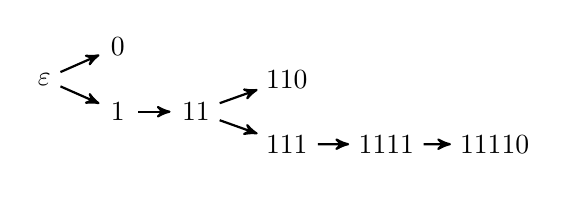
\begin{tikzpicture}[->,>=stealth',auto,thick, scale = 0.55,state/.style={circle,inner sep=2pt}]
	\node [state] at (-0.2,0) (r) {$\varepsilon$};
	\node [state] at (1.5,0.75) (n0) {$0$};
	\node [state] at (1.5,-0.75) (n1) {$1$};
	\node [state] at (3.3,-0.75) (n11) {$11$};
	\node [state] at (5.4,0) (n110) {$110$};
	\node [state] at (5.4,-1.5) (n111) {$111$};
	\node [state] at (7.7,-1.5) (n1111) {$1111$};
	\node [state] at (10.2,-1.5) (n11110) {$11110$};

	\path[->]
	(r) edge (n1)
	(r) edge (n0)
	(n1) edge (n11)
	(n11) edge (n110)
	(n11) edge (n111)
	(n111) edge (n1111)
	(n1111) edge (n11110);
\end{tikzpicture}
\end{center}
In this case, we have that $q = \{\varepsilon, 0, 1, 11, 110, 111, 1111, 11110\}$, so $q$ is a finite and prefix-closed subset of $\bB = \{0,1\}^*$. The owner of each block $b \in q \smallsetminus \{ \varepsilon\}$ is given by the  the last symbol of $b$; for instance, we have that $\owner(11) = 1$ and $\owner(11110) = 0$. Moreover, the longest path in $q$ is $\pi = \{\varepsilon, 1, 11, 111, 1111, 11110\}$, so that the blockchain of $q$ is $\pi$ (in symbols, $\bchain(q) = \pi$).
%Thus, we have that the blocks that belong to the blockchain of $q$ are $\varepsilon$, $1$, $11$, $111$, $1111$, $11110$, since these are precisely the blocks in $q$ in the path from $\varepsilon$ to $11110$ (in symbols, $\epath(\bchain(q)) = \{\varepsilon, 1, 11, 111, 1111, 11110\}$). Notice that the information about these blocks is important as the reward of each player depends on the blocks that belong to her in the blockchain. For instance, if the reward for each block is a constant $c$, then we have that the reward of player 1 is $4 c$ in $q$, as four blocks in the blockchain of $q$ belong to this player.
Finally, notice that $|q| = 8$, as $q$ is a set consisting of eight blocks.

	Assume now that $q'$ is the following state of the game:
	\begin{center}
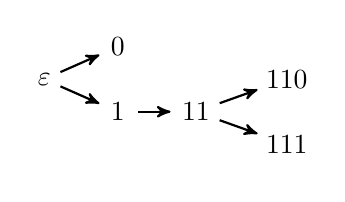
\begin{tikzpicture}[->,>=stealth',auto,thick, scale = 0.55,state/.style={circle,inner sep=2pt}]
	\node [state] at (-0.2,0) (r) {$\varepsilon$};
	\node [state] at (1.5,0.75) (n0) {$0$};
	\node [state] at (1.5,-0.75) (n1) {$1$};
	\node [state] at (3.3,-0.75) (n11) {$11$};
	\node [state] at (5.4,0) (n110) {$110$};
	\node [state] at (5.4,-1.5) (n111) {$111$};

	\path[->]
	(r) edge (n1)
	(r) edge (n0)
	(n1) edge (n11)
	(n11) edge (n110)
	(n11) edge (n111);
\end{tikzpicture}
\end{center}
In this case, we have that $\bchain(q')$ is not defined since the paths $\pi_1 = \{\varepsilon, 1, 11, 110\}$ and $\pi_2 = \{\varepsilon, 1, 11, 111\}$ are tied for the longest path in $q'$. \qed
\end{example}


Real-life bitcoin blocks also contain transactions that indicate movement of money in the system, and thus there are
several different blocks that a player $p$ can use to extend the current state when mining upon a block $b$ (e.g, depending  on the ordering of transactions, or the nonce being used to announce the block). Since we are interested primarily in miners behaviour, we just focus on the owner of the block following $b$, and do not consider the possibility of two different blocks belonging to $p$ being added on top of $b$. 
%Alternatively, if we consider the Bitcoin protocol, we could say that all the different blocks that $p$ can put on top of $b$ are considered as~equivalent.
%\juan{moving this to the reward section}
%\etienne{We may have to specify that it is under the assumption that there are no fees or that they are negligible.} \marcelo{Etienne is right about this, depending on the transactions included in the block the reward could be different. I don't think we should talk about reward here.}

\subsubsection{Actions of a miner}\label{sub:actions}
On each step, miners looking to maximize their rewards choose a block in the current state, and attempt to mine on top of this block. Thus, in each turn, each of the players race to place the next block in the state, and only one of them succeeds. The probability of succeeding is directly related to the comparative amount of hash power available to this player, the more hash power the likely it is that she will mine the next block before the rest of the players. Once a player places a block, this block is added to the current state, obtaining a different state from which the game continues.

Let $p \in \bP$. Given a block $b \in \bB$ and a state $q \in \bQ$, we denote by $\mine(p,b,q)$ an action played in the mining game in which player $p$ mines on top of block $b$. Such an action $\mine(p,b,q)$ is considered to be valid if $b \in q$ and $b\cdot p \not\in q$. The set of valid actions for player $p$ is collected in the set:
\begin{multline*}
\bA_p \ = \ \{ \mine(p,b,q) \mid b \in \bB, q \in \bQ \text{ and}\\\mine(p,b,q) \text{ is a valid action}\}.
\end{multline*}
Moreover, given $a \in \bA_p$ with $a = \mine(p,b,q)$, the result of applying $a$ to $q$, denoted by $a(q)$, is defined as the state $q \cup \{b \cdot p\}$. Finally, we denote by $\bA$ the set of combined actions for the $m$ players, that is, $\bA = \bA_0 \times \bA_1 \times \cdots \times \bA_{m-1}$.

\subsubsection{The pay-off of a miner}
For each player $p \in \bP$, we assume the existence of a pay-off function $r_p : \bQ \to \mathbb{R}$, so that the pay-off of $p$ in a state $q$ is given by $r_p(q)$. Moreover, the combined pay-off function of the game is $\bR = (r_0, r_1, \ldots, r_{m-1})$. In Section \ref{sec-pay-ut}, we discuss the implications of defining miners' pay-offs in this way, and the implications of the manner these pay-offs are accumulated in the utility function.

\subsubsection{Transition probability function}\label{sub:transi}

As a last component of the game, we assume that $\pr : \bQ \times \bA \times \bQ \to [0,1]$ is a transition probability function satisfying that for every state $q \in \bQ$ and combined action $\ba = (a_0, a_1, \ldots, a_{m-1})$ in $\bA$:
\begin{eqnarray*}\label{eq-prop}
\sum_{p=0}^{m-1} \pr(q, \ba, a_p(q)) & = & 1.
\end{eqnarray*}
Notice that if $p_1$ and $p_2$ are two different players, then for every action $a_1 \in \bA_{p_1}$, every action $a_2 \in \bA_{p_2}$ and every state $q \in \bQ$, it holds that $a_1(q) \neq a_2(q)$. Thus, we can think of $\pr(q, \ba, a_p(q))$ as the probability that player $p$ places the next block, which will generate the state $a_p(q)$. As we have mentioned, such a probability is directly related with the hash power of player $p$, the more hash power the likely it is that action $a_p$ is executed and $p$ mines the next block before the rest of the players. In what follows, we assume that the hash power of each player does not change during the mining game, which is captured by the following condition:
\begin{itemize}
\item Given $q, q' \in \bQ$ and $\ba, \ba' \in \bA$ with $\ba = (a_0, a_1$, $\ldots$, $a_{m-1})$ and $\ba' = (a'_0, a'_1, \ldots, a'_{m-1})$, for every player $p \in \bP$ it holds that $\pr(q, \ba, a_p(q)) = \pr(q', \ba', a'_p(q'))$.
\end{itemize}
Thus, we assume from now on that this condition is satisfied. In particular, for each player $p \in \bP$, we assume that that
$\pr(q, \ba, a_p(q)) = h_p$ for every $q \in \bQ$ and $\ba \in \bA$ with $\ba = (a_0, a_1, \ldots, a_{m-1})$, and we refer to $h_p$ as the hash power of player $p$.
%Moreover, we define $\bH = (h_0, h_1, \ldots, h_{m-1})$ as the hash power distribution, and we replace $\pr$ by $\bH$ in the definition of an an infinite stochastic game, so that $\Gamma = (\bP,\bA,\bQ,\bR,\bH)$.
Moreover, we assume that $h_p > 0$ for every player $p \in \bP$, as if this not the case then $p$ can just be removed from the mining game.


\subsubsection{The mining game: definition, strategy, utility and equilibrium}
Putting together the components defined in the previous sections, we have that 
%Summing up, from now on we consider 
an infinite stochastic game is a tuple $\Gamma = (\bP,\bQ,\bA,\bR,\pr)$, where $\bP$ is the set of players, $\bQ$ is the set of states, $\bA$ is the set of combined actions, $\bR$ is the combined pay-off function 
and $\pr$ is the transition probability function. 

%The pay-off function of the game denoted $\bR = (r_0,r_1 \cdots, r_{m-1})$, with $r_p : \bQ \mapsto \mathbb{R^+}$ is the pay-off function of the player $p$, represent the reward that each player receive at any state of the game. Before presenting our model for the pay-off function we have to talked about the purpose of using stochastic game as a model.

We have defined a game that can capture miners' interactions. A fundamental component of such a game is the strategy that each player decides to take, which combined determine the utility of each player. In particular, miners take actions and decide about strategies trying to maximize their utility. In this sense, a 
%stationary 
equilibrium of the game is a fundamental piece of information about miners' behavior, because such an equilibrium is a combination of players' strategies where no miner has an incentive to perform a different action. The notions of strategy, utility and stationary equilibrium are the last components of our game-theoretical characterization of mining in Bitcoin, and they are defined next. 

A Markov strategy (or just strategy) for a player $p \in \bP$ is a function $s : \bQ \rightarrow \bA_p$.
We define $\bS_p$ as the set of all strategies for player $p$, and $\bS = \bS_0 \times \bS_{1} \times \cdots \times \bS_{m-1}$ as the set of combined strategies for the game (recall that we are assuming that $\bP = \{0, 1, \ldots, m-1\}$ is the set of players).

As usual, we are interested in understanding which strategies are better than others, which we capture by the notions of  utility and equilibrium. To define these, we need some additional notation.
Let $\bs = (s_0, s_1, \ldots, s_{m-1})$ be a strategy in $\bS$. Then given $q \in \bQ$, define $\bs(q)$ as the combined action $(s_0(q), s_1(q), \ldots, s_{m-1}(q))$. Moreover, given an initial state $q_0 \in \bQ$,
the probability of reaching state $q \in \bQ$, denoted by $\pr^{\bs}(q \mid q_0)$, is defined as 0 if $q_0 \not\subseteq q$ (that is, if $q$ is not reachable from $q_0$), and otherwise it is recursively defined as follows: if $q =  q_0$, then $\pr^{\bs}(q \mid q_0) = 1$; otherwise, we have that $|q| - |q_0| = k$, with $k \geq 1$, and
$$
\pr^{\bs}(q \mid q_0) =
\sum_{\substack{q' \in \bQ \,:\\ q_0 \subseteq q' \text{ and } |q'| - |q_0| = k-1}}
 \pr^{\bs}(q' \mid q_0) \cdot \pr(q', \bs(q'), q).
 $$
In this definition, if for a player $p$ we have that $s_p(q') = a$ and $a(q') = q$, then $\pr(q', \bs(q'), q) = h_p$. Otherwise, we have that $\pr(q', \bs(q'), q) = 0$.
%Hence, consistently with the simplification described before, we can replace the transition probability function $\pr$ by the hash power distribution $\bH$ when computing $\pr^{\bs}(q \mid q_0)$.
It should be noticed that the framework just described corresponds to a Markov chain; in particular, the probability of reaching a state from an initial state is defined in the standard way for Markov chains~\cite{MU05}. However, we are not interested in the steady distribution for such a Markov chain and, thus, we do not explore more this connection in this paper.

We finally have all the necessary ingredients to define the utility of a player in a mining game given a particular strategy. As is common
when looking at personal utilities, we define it as the summation of the expected rewards, and choose
to impose a discount for future rewards using a factor $\beta \in (0,1)$.

\begin{mydef}
\label{def-utility}
The $\beta$--discounted utility of player $p$ for the strategy $\bs$ from the state $q_0$ in
the mining game, denoted by $u_p(\bs \mid q_0)$, is defined as:
\begin{eqnarray*}
u_p(\bs \mid q_0) & = & (1 - \beta) \cdot  \sum_{q \in \bQ \,:\, q_0 \subseteq q} \beta^{|q|-|q_0|} \cdot  r_p(q) \cdot \pr^{\bs}(q \mid q_0).
\end{eqnarray*}
\end{mydef}
Notice that the value $u_p(\bs \mid q_0)$ may not be defined if the series $\sum_{q \in \bQ \,:\, q_0 \subseteq q} \beta^{|q|-|q_0|} \cdot  r_p(q) \cdot \pr^{\bs}(q \mid q_0)$ diverges. To avoid this problem, from now on we assume that for every pay-off function $\bR = (r_0, \ldots, r_{m-1})$, there exists a polynomial $P$ such that $|r_p(q)| \leq P(|q|)$ for every player $p \in \bP$ and state $q \in \bQ$. Under this simple yet general condition, which is satisfied by the pay-off functions considered in this paper and in other game-theoretical formalizations of Bitcoin mining \cite{mininggames:2016}, it is possible to prove that $u_p(\bs \mid q_0)$ is a real number. 
%(see Appendix \ref{sec-conver} for a proof of this property).

As a last ingredient in our formalization, we need to introduce the notion stationary equilibrium.
Given a player $p \in \bP$, a combined strategy $\bs \in \bS$, with $\bs = (s_0,s_1, \ldots, s_{m-1})$, and a strategy $s$ for player $p$ ($s \in \bS_p$), we denote by $(\bs_{-p}, s)$ the strategy $(s_0, s_1, \ldots s_{p-1},s,s_{p+1}, \ldots, s_{m-1})$.
\begin{mydef}
A strategy $\bs$ is a $\beta$--discounted stationary equilibrium from the state $q_0$ in  the %infinite
mining game if for every player $p \in \bP$ and every strategy $s$ for player $p$ $(s \in\bS_p)$, it holds that:
\begin{eqnarray*}u_p(\bs \mid q_0)  & \geq  & u_p ((\bs_{-p},s) \mid q_0).
\end{eqnarray*}
\end{mydef}

\subsection{On the pay-off and utility of a miner}\label{sec-pay-ut}
Blockchain protocols enforce that miners receive a reward once and only once for each block they own
in the blockchain. However due to the nature of pay-off functions in stochastic game such rule can not be enforce. Indeed as the pay-off function does not rely on the history of states, for any pay-off function there exists a sequence of plays such that a miner has never received a reward for a block belonging to the blockchain, or he has received it several times. 

In this section, we show how this constraint is enforced in our framework by combining the notions of pay-off function and $\beta$--discounted utility introduced in the previous section. \etienne{We should change enforced by something just a bit weaker and it would be perfect.}

Assume that the reward obtained by a player $p$ for a block $b$ in a state $q$ such that $b \in q$ is given by $r_p(b,q)$, so that $r_p(q) = \sum_{b \in q} r_p(b,q)$. This decomposition can be done in a natural and straightforward way for the pay-off functions considered in this paper and in other game-theoretical formalizations of Bitcoin mining \cite{mininggames:2016}. We propose a pay-off where on every states, we pay miners for each of the blocks they already have in the blockchain, plus the new block they will potentially mine. Therefore for any player $p$ and any state $q$ we have that $r_p(q,b) \neq 0$ if $q \in bc(q)$ and $\owner(q) = p$. And the pay-off function verify $r_p(q) = \sum_{b \in q} r_p(b,q)$.
This model clearly puts a strong incentive in maintaining blocks in the blockchain and does not nullify the incentive to fork. The main concern is that if we consider a sequence of plays we end-up giving reward to a miner multiple times for the same block (once for each state where the block belongs to the blockchain), but to analyse the pay-off of a sequence of plays one should focus on the utility. 

Definition~\ref{def-utility} corresponds to the usual notion of average discounted utility \marcelo{A citation is needed here}. In particular, if the starting point of the game is a state $q_0$, then for every state $q$ such that $q_0 \subseteq q$, the pay-off of a player $p$ in $q$ is $\beta^{|q|-|q_0|} \cdot r_p(q)$, where $|q|-|q_0|$ is the number of steps that have to be performed to reach $q$ from $q_0$ so the discount factor $\beta^{|q|-|q_0|}$ has to be applied. The uncertainty  about reaching state $q$ from $q_0$ is taking into consideration by including the term $\pr^{\bs}(q \mid q_0)$, which tell us that the expected pay-off of player $p$ for the state $q$ is $\beta^{|q|-|q_0|} \cdot  r_p(q) \cdot \pr^{\bs}(q \mid q_0)$.
%
%As a last comment on the definition of utility, 

But notice that although this definition of expected pay-off is the natural one,
a block $b$ can be included in an infinite number of states $q$ such that $\pr^{\bs}(q \mid q_0) > 0$, which is in contradiction with the aforementioned blockhain protocol's rule that a miner receives a reward once and only once for each block she owns in the blockchain. To solve this issue, the term $(1 - \beta)$ is included in the definition of utility, as shown next.
% But the reward obtained by a player $p$ for this block $b$ should not be added more than once, which is the reason to include the term $(1 - \beta)$ in the definition of utility. Let us formalize this claim in more precise terms.
Given a combined strategy $\bs$, we can naturally define the utility of a block $b$ for a player $p$, denoted by $u_p^b(\bs \mid \{\varepsilon\})$,  as follows:
\begin{eqnarray*}
u_p^b(\bs \mid \{\varepsilon\}) & =  & (1 - \beta) \cdot  \sum_{q \in \bQ \,:\, b \in q} \beta^{|q|-1} \cdot  r_p(q,b) \cdot \pr^{\bs}(q \mid \{\varepsilon\}).
\end{eqnarray*}
For the sake of readability, we assume that the game is starting from the initial state $\{\varepsilon\}$ that consists only of the genesis block. Notice that $|\{\varepsilon\}| = 1$, so that the discount factor for a state $q$ is $\beta^{|q|-1}$. Now assume that there is a maximum value for the reward of a block $b$ for player $p$, which is denoted by $M_p(b)$. Thus, we have that there exists $q_1 \in \bQ$ such that $b \in q_1$ and $M_p(b) = r_p(b,q_1)$, and for every $q_2 \in \bQ$ such that $b \in q_2$, it holds that $r_p(b,q_2) \leq M_p(b)$. Again, such an assumption is satisfied by the pay-off functions considered in this paper and in other game-theoretical formalizations of Bitcoin mining \cite{mininggames:2016}. Then we have that:
\begin{myprop}\label{prop-ub-block}
For every player $p \in \bP$, block $b \in \bB$ and combined strategy $\bs \in \bS$, it holds that:
\begin{eqnarray*}
u^b_p(\bs \mid \{\varepsilon\}) & \leq &  \beta^{|b|} \cdot M_p(b).
\end{eqnarray*}
\end{myprop}
Thus, the utility obtained by player $p$ for a block $b$ is at most $\beta^{|b|} \cdot M_p(b)$, that is, the maximum reward that she can obtained for the block $b$ in a state multiplied by the discount factor $\beta^{|b|}$, where $|b|$ is the minimum number of steps that have to be performed to reach a state containing $b$ from the initial state $\{\varepsilon\}$. 
Moreover a miner get the maximum utility of a block if and only of this block belongs to the blockchain of any possible future state. Which make sense as it means the miner get maximal value if he can spend is money whenever he wants to.

\iffalse
Given a player $p$ and a combined strategy $\bs$, we have that: 
\begin{eqnarray*}
u_p(\bs \mid \{\varepsilon\})  & =  & \sum_{b \in \bB} u^b_p(\bs \mid \{\varepsilon\}).
\end{eqnarray*}
Therefore, we know from Proposition \ref{prop-ub-block} that the reward of $p$ for a block $b$ is not accumulated more than once in the utility of $p$ for the combined strategy $\bs$. In fact, we obtained as a corollary of Proposition \ref{prop-ub-block} that:
\begin{mycor}\label{cor-ub-ut}
For every player $p \in \bP$ and combined strategy $\bs \in \bS$, it holds that:
\begin{eqnarray*}
u_p(\bs \mid \{\varepsilon\}) & \leq &  \sum_{b \in \bB} \beta^{|b|} \cdot M_p(b).
\end{eqnarray*}
\end{mycor}
\fi



%Blockchain protocol rules enforce that miners receive a reward once and only once for each block they own
%in the blockchain, therefore we want to build a pay-off function which respect this constraint. 
%As we only have a access to the reward of states through the pay-off function, we express the reward of a block $b$ for a player $p$ in a state $q$ as the difference between the reward of $p$ in $q$ and the reward of $p$ in $q$ if the owner of $b$ was different.
%In order to formally define the notion of reward of a block we need to introduce a few notation. 
%\begin{mydef}
%Let $q \in \bQ$ a state, $p \in \bP$ a players and $b \in q$ a block we call substitution the state denoted $sub(b,q,p)$ such that $b' \in sub(b,q,p)$ if and only if $b' \in q \land b \not \preceq b'$ or $\exists b'' \in q, b \preceq b'', \forall i \neq |b|, b''[i] = b'[i], b'[i] = p$.
%\end{mydef}
%Informally $sub(b,q,p)$ corresponds to the same state as $q$ expect that the owner of the block $b$ is $p$.
%Now we can formally define the reward of a block.
%\begin{mydef}
%The reward of a block for player $p$ is a function $r_p : \bQ  \times \B \mapsto \mathbb{R}$ such that:
%\begin{equation*}
%r_p(q,b) = r_p(q) - r_p(sub(b,q,p')) \textit{ with } p' \neq p
%\end{equation*}
%\end{mydef}
%
%We define a path of the game as sequence $\Pi = \epsilon,q_1,q_2,\cdots$ of states $q_i \in \bQ$, where if $q_{i+1} \in \bQ$ then there exists $p \in \bP$ and $a_p \in \bA_p$ such that $q_{i+1}= a_p(q_i)$.
%
%\begin{myprop}\label{prop:impo}
%For any $r_p: \bQ  \mapsto \mathbb{R}$, there exist a path of the game $\Pi$ such that \ref{eq:never} or \ref{eq:multiple} is verified:
%\begin{equation}\label{eq:never}
%\exists q_i \in \Pi,\exists b \in bc(q_i), \forall q_{j} r_p(q_{j},b) = 0
%\end{equation}
%\begin{equation}\label{eq:multiple}
%\exists b \in \B, \exists q_i,q_{j} \in \Pi, q_i \neq q_{j}, r_p(q_i,b) \neq 0,  r_p(q_{j},b) \neq 0
%\end{equation}
%\end{myprop}
%
%Proposition \ref{prop:impo} tell us that it is impossible to build a pay-off function such that miners receive reward once and only once for each block they own in the blockchain. \textit{Note that proposition \ref{prop:impo} holds even if we consider more general pay-off functions from $\bQ \times \bA$ to $\mathbb{R}$, we only considered functions from $\bQ$ to $\mathbb{R}$ to simplify notation.}
%
%%\etienne{This part can go in relative work now i guess ? or a slightly different and shorter version. (To discuss with Marcelo)}
%%A pay-off function has been proposed in \cite{}, such that at every level of the state's tree only the first block which has been confirmed by $\delta \in \mathbb{N}$ blocks give reward to his owner. Due to this constraint if a fork longer than $\delta$ blocks would happen, some blocks belonging to the new blockchain won't give any reward to their owners. As a matter of fact the model nullify the incentive of performing a fork longer than $\delta$ \cite{}. One could argue that a fork longer than $\delta$ would destroy the market confidence and therefore can be ignored. It might be the case with the current state of crypto-currencies, but as the technology become more widely adopted (government or bank), such argument can not be use any-more.
%
%Hence we propose a heuristic where on every states, we pay miners for each of the blocks they already have in the blockchain, plus the new block they will potentially mine. Therefore for any player $p$ and any state $q$ we have that $r_p(q,b) \neq 0$ if $q \in bc(q)$ and $\owner(q) = p$. And the pay-off function verify\begin{equation*}
%\forall q \in \bQ, r_p(q)= \sum_{b \in \B} r_p(q,b)
%\end{equation*} 
%This model puts a strong incentive in maintaining blocks in the blockchain and does not nullify the incentive to fork. The main concern regarding this pay-off model, is that we end-up giving reward to a miner multiple times for the same block (once for each state where the block belongs to the blockchain). But as we are working with the utility defined above \ref{}, the problem "disappear".
%
%\begin{myprop}\label{prop:bound}
%Assume $M_p(b) = max(\{r_p(q,b) \mid q \in \bQ \})$ is finite and $\forall q \in \bQ, r_p(q) = \sum_{b \in \B} r_p(q,b)$ then:
%\begin{equation*}
%u_p(\bs \mid \{\varepsilon\}) \leq   \sum_{b \in \bB} \beta^{|b|} \cdot M_p(b)
%\end{equation*}
%\end{myprop}
%\iffalse
%\begin{proof}
%We conclude this section by going deeper into the definition of utility, given the key role it plays in our framework.
%Definition~\ref{def-utility} corresponds to the usual notion of average discounted utility \marcelo{A citation is needed here}. In particular, if the starting point of the game is a state $q_0$, then for every state $q$ such that $q_0 \subseteq q$, the pay-off of a player $p$ in $q$ is $\beta^{|q|-|q_0|} \cdot r_p(q)$, where $|q|-|q_0|$ is the number of steps that have to be performed to reach $q$ from $q_0$ so the discount factor $\beta^{|q|-|q_0|}$ has to be applied. The uncertainty  about reaching state $q$ from $q_0$ is taking into consideration by including the term $\pr^{\bs}(q \mid q_0)$, which tell us that the expected payoff for the state $q$ is $\beta^{|q|-|q_0|} \cdot  r_p(q) \cdot \pr^{\bs}(q \mid q_0)$.
%%
%As a last comment on the definition of utility, notice that a block $b$ can be included in an infinite number of states $q$ such that $\pr^{\bs}(q \mid q_0) > 0$. But the reward obtained by a player $p$ for this block $b$ should not be added more than once, which is the reason to include the term $(1 - \beta)$ in the definition of utility. Let us formalize this claim in more precise terms.
%
%Assume that the reward obtained by a player $p$ for a block $b$ in a state $q$ is given by $r_p(b,q)$, so that $r_p(q) = \sum_{b \in q} r_p(b,q)$. Notice that such decomposition can always be done; in fact, it can be done in a natural and straightforward way for the pay-off functions considered in this paper and in other game-theoretical formalizations of Bitcoin mining \cite{mininggames:2016}. Then we have:
%\begin{align*}
%u_p(\bs \mid \{\varepsilon\}) & =  (1 - \beta) \cdot  \sum_{q \in \bQ} \beta^{|q|-|\{\varepsilon\}|} \cdot  r_p(q) \cdot \pr^{\bs}(q \mid \{\varepsilon\})\\
%& =  (1 - \beta) \cdot \sum_{q \in \bQ} \beta^{|q|-1} \cdot  \bigg(\sum_{b \in q} r_p(b,q) \bigg) \cdot \pr^{\bs}(q \mid \{\varepsilon\})\\
%& = (1 - \beta) \cdot \sum_{b \in \bB} \sum_{q \in \bQ \,:\, b \in q} \beta^{|q|-1} \cdot r_p(b,q) \cdot \pr^{\bs}(q \mid \{\varepsilon\}).
%\end{align*}
%For the sake of readability, we assume that the game is starting from the initial state $\{\varepsilon\}$ that consists only of the genesis block. Notice that $|\{\varepsilon\}| = 1$, so that the discount factor for a state $q$ is $\beta^{|q|-1}$. Now assume that there is a maximum value for the reward of a block $b$ for player $p$, which is denoted by $M_p(b)$. Thus, we have that there exists $q_1 \in \bQ$ such that $b \in q_1$ and $M_p(b) = r_p(b,q_1)$, and for every $q_2 \in \bQ$ such that $b \in q_2$, it holds that $r_p(b,q_2) \leq M_p(b)$. Again, such an assumption is satisfied by the pay-off functions considered in this paper and in other game-theoretical formalizations of Bitcoin mining \cite{mininggames:2016}. Then we have that:
%\begin{align*}
%&\sum_{b \in \bB} \sum_{q \in \bQ \,:\, b \in q} \beta^{|q|-1} \cdot r_p(b,q) \cdot \pr^{\bs}(q \mid \{\varepsilon\})
%\ \leq \\
%&\hspace{40pt}  \sum_{b \in \bB} \sum_{q \in \bQ \,:\, b \in q} \beta^{|q|-1} \cdot M_p(b) \cdot \pr^{\bs}(q \mid \{\varepsilon\}) \ =\\
%&\hspace{40pt}  \sum_{b \in \bB} M_p(b) \cdot\bigg(\sum_{q \in \bQ \,:\, b \in q} \beta^{|q|-1}  \cdot \pr^{\bs}(q \mid \{\varepsilon\})\bigg) \ \leq\\
%&\hspace{40pt}  \sum_{b \in \bB} M_p(b) \cdot\bigg(\sum_{q \in \bQ \,:\, |q| \geq |b|+1} \beta^{|q|-1}  \cdot \pr^{\bs}(q \mid \{\varepsilon\})\bigg) \ = \\
%&\hspace{40pt}  \sum_{b \in \bB} M_p(b) \cdot\bigg(\sum_{i=|b|+1}^\infty \sum_{q \in \bQ \,:\, |q| = i} \beta^{|q|-1}  \cdot \pr^{\bs}(q \mid \{\varepsilon\})\bigg) \ = \\
%&\hspace{40pt}  \sum_{b \in \bB} M_p(b) \cdot\bigg(\sum_{i=|b|+1}^\infty \beta^{i-1} \cdot \sum_{q \in \bQ \,:\, |q| = i} \pr^{\bs}(q \mid \{\varepsilon\})\bigg).
%\end{align*}
%By the definition of the transition probability function $\pr^{\bs}$, it is straightforward to prove that $\sum_{q \in \bQ \,:\, |q| = i} \pr^{\bs}(q \mid \{\varepsilon\}) = 1$. Hence, we conclude that:
%\begin{align*}
%&\sum_{b \in \bB} M_p(b) \cdot\bigg(\sum_{i=|b|+1}^\infty \beta^{i-1} \cdot \sum_{q \in \bQ \,:\, |q| = i} \pr^{\bs}(q \mid \{\varepsilon\})\bigg) \ = \\
%&\hspace{60pt}  \sum_{b \in \bB} M_p(b) \cdot\bigg(\sum_{i=|b|+1}^\infty \beta^{i-1}\bigg) \ = \\
%&\hspace{60pt}  \sum_{b \in \bB} M_p(b) \cdot \beta^{|b|} \cdot \bigg(\sum_{j=0}^\infty \beta^{j}\bigg) \ = \\
%&\hspace{60pt}  \sum_{b \in \bB} M_p(b) \cdot \beta^{|b|} \cdot \frac{1}{1-\beta},
%\end{align*}
%where $|b|$ is the length of block $b$ considered as a string. Therefore, we finally conclude that:
%\begin{eqnarray*}
%u_p(\bs \mid \{\varepsilon\}) & \leq &  \sum_{b \in \bB} \beta^{|b|} \cdot M_p(b).
%\end{eqnarray*}
%Thus, the pay-off obtained by player $p$ for a block $b$ is at most $\beta^{|b|} \cdot M_p(b)$, that is, the maximum reward that she can obtained for the block $b$ in a state multiplied by the discount factor $\beta^{|b|}$, where $|b|$ is the minimum number of steps that have to be performed to reach a state containing $b$ from the initial state $\{\varepsilon\}$.
%
%\marcelo{The justification of the utility function is long, we can move the proof to the appendix and only keep the bound $u_p(\bs \mid \{\varepsilon\}) \leq \sum_{b \in \bB} \beta^{|b|} \cdot M_p(b)$.}
%\martin{Agree, would give it as a proposition to show that this is not over-counting blocks, and leave the proof to the appendix.}
%
%%Along the paper we will also consider games ending in a finite number of steps. For these games we redefine the notion of $\beta$-discounted utilities by summing up the rewards only up to $n$, and define the notion of a $\beta$-discounted equilibrium accordingly.
%%\marcelo{We are not going to consider games ending in a finite number of steps in this paper, right?}
%
%%\marcelo{In these definitions we are assuming that $u_p(\bs \mid q_0)$ is defined, which could not be the case if the series diverges. We should say something about this.}
%%\francisco{True. Something like ``$r$ is a decreasing function and card$(Q)$ is controlled by $p^{|q|}$'' (worst case scenario, every player forks), so we should be OK.}
%\end{proof}
%\fi
%
%If we extend the notion of utility to define the utility of a specific block, which correspond to the expected value a block would bring to a player, under a combined strategy.
%\begin{mydef}
%The utility of a block $b \in \B$ for a player $p \in \bP$ and a combined strategy $\bs \in \bS$ from a state $q_0 \in \bQ$ denoted $u_p^bu_p^b(\bs \mid q_0)$ is defined as:
%\begin{equation*}
%u_p^b(\bs \mid q_0) =  (1 - \beta) \cdot  \sum_{q \in \bQ \,:\, q_0 \subseteq q} \beta^{|q|-|q_0|} \cdot  r_p(q,b) \cdot \pr^{\bs}(q \mid q_0).
%\end{equation*}
%Moreover if we assume $\forall q \in \bQ, r_p(q) = \sum_{b \in \B} r_p(q,b)$ then:
%\begin{equation*}
%u_p(\bs \mid \{\varepsilon\}) =   \sum_{b \in \bB} u^b_p(\bs \mid \{\varepsilon\})
%\end{equation*}
%\end{mydef}
%
%
%Using property \ref{prop:bound} we can conclude\etienne{Actually it is not immediate at all, too bad ;s can u have that ?}:
%\begin{mylem}
%If we assume $\forall q \in \bQ, r_p(q) = \sum_{b \in \B} r_p(q,b)$ then for any block $b$, and player $p$ we have:
%\begin{equation*}
%u_p^b(\bs \mid \{\varepsilon\}) \leq \beta^{|b|} \cdot M_p(b)
%\end{equation*}
%\end{mylem}
%
%Therefore the utility bring by a block is at most the reward of the block. Intuitively a miner get the maximum utility of a block if and only of this block belongs to the blockchain of any possible future state. Which make sense as it means the miner get maximal value if he can spend is money whenever he wants to.
%
%\etienne{A word about the fact we dont care about the delay rule if and only if we keep the discusion about the other paper in this section otherwise can go in future work, conclusion or even in the specific constant and discounted reward (The definition i have given is generic enough to dont care about delay)}



%
%\iffalse
%
%\subsection{Pay-off of a miner (extended version)}
%
%
%\etienne{I still have to work on the actual wording, but i think it will look like that. I choosed to push the graph in appendix for space reasons, what do u think ?}
%
%In stochastic game,the pay-off of a player $p \in \bP$, is given by a function $r_p: \bQ \times \bA \mapsto \mathbb{R}$, and the payoff function of the game is $\bR = (r_0, r_1, \ldots, r_{m-1})$.
%But how should the function $r_p(q,\ba)$ look like? Recall that one of the rules of bitcoin is that the money can only
%be spent when it is given in blocks that are part of the blockchain. Thus, the first idea that comes into mind is to
%reward players every time they put a block in the blockchain. However, this is not a good function, as it is not possible to build a pay-off function which rewards them once and only once for each block in the blockchain (see example \ref{eximpo}).
%
%\begin{myex}
%\label{eximpo}
%\begin{figure}
%\begin{center}
%\begin{tikzpicture}[->,>=stealth',auto,thick, scale = 0.55,state/.style={circle,inner sep=2pt}]
%
%    % The graph A
%    \node [state] at (3.5,2.25) (name1) {$(q_w,\ba_w)$};
%	\node [state] at (0,1.25) (Ra0) {$\varepsilon$};
%	\node [state] at (1.5,0.5) (0a0) {$0$};
%	\node [state] at (1.5,1.25) (1a0) {$1$};
%	\node [state] at (3,1.25) (11a0) {$11$};
%	\node [state] at (5.5,1.25) (111a0) {$111$};
%
%	 % The graph A
%	\node [state] at (0,-2.25) (Ra1) {$\varepsilon$};
%	\node [state] at (1.5,-1.5) (0a1) {$1$};
%	\node [state] at (1.5,-2.25) (1a1) {$0$};
%	\node [state] at (3,-2.25) (11a1) {$00$};
%	\node [state] at (5.5,-2.25) (111a1) {$000$};
%	\node [state] at (3.5,-0.5) (name2) {$(q_l,\ba_l)$};
%
%	% The graph A
%	\node [state] at (7,0) (Ra) {$\varepsilon$};
%	\node [state] at (8.5,0.75) (1a) {$1$};
%	\node [state] at (8.5,-0.75) (0a) {$0$};
%	\node [state] at (10,0.75) (11a) {$11$};
%	\node [state] at (10,-0.75) (00a) {$00$};
%	\node [state] at (12.5,0.75) (111a) {$111$};
%	\node [state] at (12.5,-0.75) (000a) {$000$};
%	\node [state] at (10.5,-1.75) (name3) {$(q_t,\ba_t)$};
%
%	% Graph edges
%	\path[->]
%	(Ra) edge (1a)
%	(Ra) edge (0a)
%	(1a) edge (11a)
%	(0a) edge (00a)
%	(Ra1) edge (1a1)
%	(1a1) edge (11a1)
%	(Ra0) edge (1a0)
%	(1a0) edge (11a0)
%	;
%
%	% Graph edges
%	\path[dashed,blue]
%	(Ra1) edge (0a1)
%	(11a) edge (111a)
%	(11a0) edge (111a0)
%	;
%
%	\path[dashed,red]
%	(Ra0) edge (0a0)
%	(00a) edge (000a)
%	(11a1) edge (111a1)
%	;
%
%
%\end{tikzpicture}
%\end{center}
%\caption{An example showing that I should want to try to compete when some other player forks on my blocks. \label{fig-impo}}
%\end{figure}
%
%
%
%Consider a pay-off function $r_1$ for player $1$, it is immediate to understand that in the situation described by $q_l$ the value $r_1(q_l,\ba_l)$ should be $0$, indeed player $1$ did not put any new block in the blockchain. While in the situation described in $q_w$, $r_1(q_w,\ba_w)$ should reward the player $1$ for his block $111$.
%\\Now consider the tie situation described in $q_t$. What should be the value of $r_1(q_t,\ba_t)$? Either $r_1(q_t,\ba_t)$ only rewards player 1 for his block $111$, and if $q_t$ has been reach through $q_l$ then he would never has been paid for the block $1$. Or $r_1(q_t,\ba_t)$ rewards player 1 for every blocks involved in the tie and if $q_t$ is reach trough $q_w$, he would have been paid twice for the blocks $1$ and $11$. The pay-off not relying on the history of states, cannot distinguish those two situations hence it is not possible to build a pay-off function which pay once and only once the player for each block in the blockchain.
%
%\end{myex}
%
%Ideally, one would like to reward players according to the blocks they have in the blockchain when the game terminates (or the limit of that number, in the case of infinite games). The problem is that we cannot really know what this pay-off will be until the game is actually finished, and thus we cannot model this pay-off in our stochastic game setting.
%What we do instead is to use a heuristic for this reward called cumulative pay-off model and denoted $r_p^c(.)$. On each turn, we pay miners a constant $c$ for each of the blocks they already have in the blockchain, plus the new block they have potentially mining them. This clearly puts a strong incentive in maintaining blocks, but also on mining new blocks on the blockchain.
%\\Note that in the general case a pay-off is a function from $\bQ \times \bA$ to $\mathbb{R}$, in our model the pay-off of player $p$ does not depend on the action of other players. Hence we extend the definition of the cumulative pay-off function such that for any state $q$ and any player $p$ we have $r_p^c(q) = r_p^c(q',(\ba,a_p))$ with $q' = q \setminus b$ and $a_p = mine(p,b,q')$. We also consider a function where the reward for each new block in the blockchain decreases by a constant factor $\alpha$. We will formally define our cumulative payoff functions in the following sections.
%
%
%The main concern regarding this pay-off function called cumulative pay-off, is that the early blocks may have a lot more value than the later ones (not because of a decreasing reward, but because early blocks are counted multiple times).
%In order to show that this problem is not as strong as it might seems, we compared the sum of the rewards obtained under the cumulative, relative \cite{} and absolute \cite{} pay-off models on pseudo-randomly generated  blockchains. We considere a fix number of blocks distrubuted upon players $\bP$ and we assume they always mined upon the blockchain (default behaviour). Therefore the only variable between two iterations is the position of the blocks own by each players. The total number of blocks at the end of each iteration is 100.000 and we have done 1000 iterations. Let $i \in \{1\cdots 1000\}$, we denote by $q_i$ the final state of the iteration. For any state $q \subseteq q_i$ and any player $p \in \bP$ we denote $r_p^a(q)$ resp. $r_p^r(q)$ the absolute resp. relative pay-off function. We have that $r_p^a(q) = c$ if $owner(bc(q)) = p$ and $r_p^a(q) = 0$ otherwise. And that $r_p^r(q) = \frac{c}{|q|}$ if $owner(bc(q)) = p$ and $r_p^r(q) = 0$ otherwise. Finally with $$R_p^x(q_i) = \frac{\sum\limits_{q \subseteq q_i} r_p^x(q)}{\sum\limits_{p' \in \bP}\sum\limits_{q \subseteq q_i} r_{p'}^x(q)} $$ we call maximum difference the value:\\ $\underset{p \in \bP}{max}\left(\underset{{i \in \{1 \cdots 10
%00\}}}{max}(R_p^x(q_i)) - \underset{{i \in \{1 \cdots 10
%00\}}}{min}(R_p^x(q_i))\right)$\\and average difference the value: $\underset{{i,i' \in \{1 \cdots 10
%00\}}}{average}(|R_p^x(q_i) - R_p^x(q_{i'})|) $.
%
%\begin{figure}
%\begin{tabular}{c|c|c|}
%. & maxium difference & average difference   \\
%\hline
%constant pay-off & 0 & 0 \\
%\hline
%relative pay-off & x.x &  x.x \\
%\hline
%cumulative pay-off &  x.x &  x.x \\
%\end{tabular}
%\caption{Results of the simulation for absolute, relative and cumulative models}
%\end{figure}
%
%As you can see in the table \ref{}, the cumulative model yields to a behaviour inbetween the constant and relative models. Therefore, even if the value for the early blocks of the blockchain is higher than the value for the later ones, the difference between them is reasonable. More details and results about this experimentation are available in appendix \ref{}.
%
%An other possible pay-off function presented in \cite{}, introduced a delay $d$ before rewarding a player for a block. Moreover this pay-off also insure that only one block for each depth is going to receive a payment (the first one for which the delay $d$ is achieve). It is really close to the bitcoin protocol as miners have to wait 100 blocks in order to use their coin-base transaction bitcoins, however the constraint that only one block per depth can be paid nullify the incentive of performing a fork longer than $d$. One could argue that a fork longer than $d$ would destroy the market confidence hence the value and therefore can be ignored. It might be the case with the current state of crypto-currencies, but if the technology become more widely adopted (government or bank), such argument can not be use any-more.
%
%
%
%%The other issue is what to do when the blockchain is contested, and there are at least two paths sharing the maximal length. A simple solution
%%would be to declare that players receive no pay-off when this happens. But again, this would lead to strange behaviours in which players with several blocks buried deep in the blockchain would receive no reward for this blocks because of a contest in the newer parts of the blockchain.
%%In order to avoid this scenario, we choose to maintain the reward for blocks buried deep in the blockchain even when there is a contest,
%%and formalise this as follows.
%\fi
%
%\iffalse
%
%\begin{myex}
%\label{eximpo}
%\begin{figure}
%\begin{center}
%\begin{tikzpicture}[->,>=stealth',auto,thick, scale = 0.55,state/.style={circle,inner sep=2pt}]
%
%    % The graph A
%    \node [state] at (3.5,2.25) (name1) {$(q_w,\ba_w)$};
%	\node [state] at (0,1.25) (Ra0) {$\varepsilon$};
%	\node [state] at (1.5,0.5) (0a0) {$0$};
%	\node [state] at (1.5,1.25) (1a0) {$1$};
%	\node [state] at (3,1.25) (11a0) {$11$};
%	\node [state] at (5.5,1.25) (111a0) {$111$};
%
%	 % The graph A
%	\node [state] at (0,-2.25) (Ra1) {$\varepsilon$};
%	\node [state] at (1.5,-1.5) (0a1) {$1$};
%	\node [state] at (1.5,-2.25) (1a1) {$0$};
%	\node [state] at (3,-2.25) (11a1) {$00$};
%	\node [state] at (5.5,-2.25) (111a1) {$000$};
%	\node [state] at (3.5,-0.5) (name2) {$(q_l,\ba_l)$};
%
%	% The graph A
%	\node [state] at (7,0) (Ra) {$\varepsilon$};
%	\node [state] at (8.5,0.75) (1a) {$1$};
%	\node [state] at (8.5,-0.75) (0a) {$0$};
%	\node [state] at (10,0.75) (11a) {$11$};
%	\node [state] at (10,-0.75) (00a) {$00$};
%	\node [state] at (12.5,0.75) (111a) {$111$};
%	\node [state] at (12.5,-0.75) (000a) {$000$};
%	\node [state] at (10.5,-1.75) (name3) {$(q_t,\ba_t)$};
%
%	% Graph edges
%	\path[->]
%	(Ra) edge (1a)
%	(Ra) edge (0a)
%	(1a) edge (11a)
%	(0a) edge (00a)
%	(Ra1) edge (1a1)
%	(1a1) edge (11a1)
%	(Ra0) edge (1a0)
%	(1a0) edge (11a0)
%	;
%
%	% Graph edges
%	\path[dashed,blue]
%	(Ra1) edge (0a1)
%	(11a) edge (111a)
%	(11a0) edge (111a0)
%	;
%
%	\path[dashed,red]
%	(Ra0) edge (0a0)
%	(00a) edge (000a)
%	(11a1) edge (111a1)
%	;
%
%
%\end{tikzpicture}
%\end{center}
%\caption{An example showing that I should want to try to compete when some other player forks on my blocks. \label{fig-impo}}
%\end{figure}
%
%Consider a pay-off function $r_1$ for player $1$, it is immediate to understand that in the situation described by $q_l$ the value $r_1(q_l,\ba_l)$ should be $0$, indeed player $1$ did not put any new block in the blockchain. While in the situation described in $q_w$, $r_1(q_w,\ba_w)$ should reward the player $1$ for his block $111$.
%\\Now consider the tie situation described in $q_t$. What should be the value of $r_1(q_t,\ba_t)$? Either $r_1(q_t,\ba_t)$ only rewards player 1 for his block $111$, and if $q_t$ has been reach through $q_l$ then he would never has been paid for the block $1$. Or $r_1(q_t,\ba_t)$ rewards player 1 for every blocks involved in the tie and if $q_t$ is reach trough $q_w$, he would have been paid twice for the blocks $1$ and $11$. The pay-off not relying on the history of states, cannot distinguish those two situations hence it is not possible to build a pay-off function which pay once and only once the player for each block in the blockchain.
%
%\end{myex}
%\fi

	%!TEX root = main.tex


\section{Equilibria in games with constant payoff}
\label{sec-const_rew}

The first version of the game we analyse is when the payoff function $r_p(q)$ pays each block in the blockchain the same amount $c$. While this does not reflect the reality of the Bitcoin protocol, this simplification serves as a good baseline for future results, and it establishes the main techniques we will use. Furthermore, the results we obtain here could serve as a good recommendation of how the Bitcoin protocol can be modified in order to enforce fair behaviour of the miners when the block reward becomes insignificant.
\marcelo{We need to change this considering the more general view of our framework for cryptocurrencies.}

\subsection{Defining constant pay-off}
When considering the constant reward $c$ for each block, $r_p(q)$ will equal $c$ times the number of blocks owned by $p$ in the blockchain $\bchain(q)$ of $q$, when the latter is defined. On the other hand, when $\bchain(q)$ is not defined it might seem tempting to simply define $r_p(q) = 0$. However, even if there is more than one longest path from the root of $q$ to its leaves, it might be the case that all such paths share a common subpath. In fact, this often happens in the Bitcoin's network, when two blocks were mined on top of the same block (with a small time delay). While in this situation the blockchain is not defined, the miners know that they will at least be able to collect their reward on the portion of the state these two paths agree on. Figure \ref{fig-simple-fork} illustrates this situation. 

\begin{figure}
\begin{center}
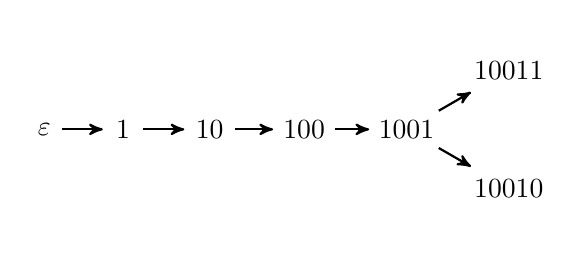
\begin{tikzpicture}[->,>=stealth',auto,thick, scale = 1.0,state/.style={circle,inner sep=2pt}]

    % The graph
	\node [state] at (0,0) (R) {$\varepsilon$};
	\node [state] at (1,0) (1) {$1$};
	\node [state] at (2.1,0) (10) {$10$};
	\node [state] at (3.3,0) (100) {$100$};
	\node [state] at (4.6,0) (1001) {$1001$};
	\node [state] at (5.9,0.75) (10011) {$10011$};
	\node [state] at (5.9,-0.75) (10010) {$10010$};	
	
	% Graph edges
	\path[->]
	(R) edge (1)
	(1) edge (10)
	(10) edge (100)
	(100) edge (1001)
	(1001) edge (10011)
	(1001) edge (10010)
	;  	
	


\end{tikzpicture} 
\end{center}
\caption{Although two paths are competing to become a blockchain, the blocks up to 1001 will contribute to the reward in each case. \label{fig-simple-fork}}
\end{figure}

In order to model the aforementioned scenario we need to introduce some notation.
Recall that a block $b$ is a string over the alphabet $\bP$, and we use notation $|b|$ for the length of $b$ as a string. Moreover, given blocks $b_1, b_2$, we use notation $b_1 \preceq b_2$ to indicate that $b_1$ is a prefix of $b_2$  when considered as strings. Then we define: 
\begin{eqnarray*}
\longest(q) & = & \{ b \in q \mid \text{for every } b' \in q: |b'| \leq |b|\}\\
\meet(q) & = & \{b \in q \mid \text{for every } b' \in \longest(q): b \preceq b'\}.
\end{eqnarray*}
Intuitively, $\longest(q)$ contains the leaves of all paths in the state $q$ that are currently competing for the blockchain, and $\meet(q)$ is the path from the genesis block to the last block for which all these paths agree on. For instance, if $q$ is the state from Figure~\ref{fig-simple-fork}, then we have that $\longest(q)=\{10011,10010\}$, and $\meet(q)=\{\varepsilon, 1, 10, 100, 1001\}$. Notice that $\meet(q)$ is well defined as $\preceq$ is a linear order on the finite and non-empty set $\{b \in q \mid \text{for every } b' \in \longest(q): b \preceq b'\}$. Also notice that $\meet(q)=\bchain(q)$, whenever $\bchain(q)$ is defined.


As mentioned before, the pay-off function will reward a player for the blocks in $\meet(q)$. Thus, to define the pay-off, we need to identify who is the owner of each one of these blocks, which is done by considering the function $\chi_p$, for each $p \in \bP$. More precisely, given $b \in \bB$, we have that:
\begin{eqnarray*}
\chi_p(b) & = & 
\begin{cases}
1 & \text{if } \owner(b) = p\\
0 & \text{otherwise}
\end{cases}
\end{eqnarray*}
We can finally define the payoff function we consider in this section, which we call \textbf{constant reward}. For a player $p$, we define it as 
\begin{eqnarray*}
r_p(q) & = & 
{\displaystyle c \cdot \sum_{b \in \meet(q)} \chi_p(b),}
\end{eqnarray*}
\martin{this reads odd since we do not use meet here. Is it correct?} \marcelo{I don't understand this comment, meet is used in the expression above.}
where $c$ is a positive real number. As mentioned above, this function is well defined since $\meet(q)$ always exists. Moreover, if $q$ has a blockchain, then we have that $\meet(q) = \bchain(q)$ and, hence, the pay-off function is defined for the blockchain of $q$.
% when the latter is defined for the state $q$.
%Here we use notation $b[i]$ for the $i$-th symbol in $b$, where $i \in \{1, \ldots, |b|\}$. 
% and $d \in \mathbb{N}$. Here the number $d$ is the amount of confirmations needed to spend the block (6 in the case of Bitcoin).
 
 \subsection{The default strategy maximizes the utility}

Let us start with analysing the most obvious strategy for all players: regardless of what everyone else does, keep mining on the blockchain, which is called the \emph{default} strategy.
More precisely, a player following the default strategy tries to mine upon the final block that appears in the blockchain of a state $q$. If the blockchain in $q$ does not exist, meaning that there are al least two longest paths from the genesis block, then the player tries to mine on the final block of one of these paths according to her rewards in them; she chooses the one that maximizes her reward, which in the case of constant reward means the path that contains the largest number of blocks belonging to her (if there is more than one of these paths, then between the final blocks of these paths she chooses the first according to a lexicographic order on the strings in $\{0, \ldots, m-1\}^*$). 
Notice that this is called the default strategy as it reflects the desired behaviour of the miners participating in the Bitcoin network.  For a player $p$, let us denote this strategy 
by $\df_p$, and consider the combined strategy $\cdf = (\df_0,\df_1,\dots,\df_{m-1})$. 
%Notice that under this strategy, each state $q$ consists of a single path from the genesis block $\varepsilon$ to the final block in $\bchain(q)$.

We can now easily calculate the utility of player $p$ under $\cdf$. Intuitively, a player $p$ will receive a fraction $h_p$ of the next block that is being placed in the blockchain, corresponding to her hash power. Therefore, at stage $i$ of the mining game, $i$ blocks will be placed in the blockchain defined by the game, and the expected amount of blocks owned by the player $p$ will be $h_p\cdot i$. This means that the total utility for player $p$ amounts to 
$$u_p(\cdf \mid \varepsilon) \ \ = \ \ (1 - \beta) \cdot h_p \cdot c\cdot \sum_{i=0}^{\infty}i \cdot \beta^{i} \ \ =  \ \ h_p\cdot c \cdot \frac{\beta}{(1-\beta)}.$$

%% Juan: I think it is way too nahive to put the analytical form of this
%$$u_p(\bs \mid q_0) = c\cdot h_p \cdot \sum_{i=0}^{\infty}i \cdot \beta^{i} \text{,}\ \ \ \ \text{ which evaluates to }\frac{c\cdot h_p}{(1-\beta)^2}.$$ %(recall that $q_0$ is the genesis block). 

The question then is: can any player do better? As we show in the following theorem, the answer is no as the default strategy maximizes the utility. 
\begin{mythm}\label{thm-conts_dom_str}
Let $p$ be a player, $\beta$ be a discount factor in $(0,1)$ and $u_p$ be the utility function defined in terms of $\beta$. Then for every combined strategy $\bs$:
\begin{eqnarray*}
u_p(\bs \mid \varepsilon) & \leq & u_p(\cdf \mid \varepsilon)
\end{eqnarray*}
\end{mythm} 

\begin{proof}
Let $\bs= (s_0, \ldots, s_{m-1})$ be an arbitrary combined strategy, and define $Q_\bs = \{q \in \bQ \mid \pr^\bs(q \mid \varepsilon) > 0\}$. Thus, $Q_\bs$ is the set of all states that can be reached from the genesis block using the combined strategy $\bs$. For example, we have that $Q_\cdf$ is the set of states $q$ such that $q$ consists of a single path from the genesis block to the final block in $\bchain(q)$.
Moreover, define a mapping $\sigma: Q_{\bs} \rightarrow 2^{Q_\cdf}$ as follows. Given two states $q_1, q_2$, we say that $q_2$ can be reached from $q_1$ in one step if $q_2 = q_1 \cup \{ b \cdot p' \}$, where $b \in \bB$, $p' \in \bP$ and $b \cdot p' \not\in q_1$ (recall that $\bB = \{0, \ldots, m-1\}^*$ and $\bP = \{0, \ldots, m-1\}$); that is, we have that $q_2$ can be reached from $q_1$ in one step  if $q_2$ is the result of applying action $\mine(p', b, q_1)$, where $\mine(p', b, q_1)$ is a valid action for player $p'$. 
Then for each state $q \in Q_{\bs}$, consider all distinct sequences $\rho = q_0,\dots,q_n$ such that $q_{i+1}$ can be reached from 
$q_i$ in one step ($i \in \{1, \ldots, n-1\}$), $q_0 = \varepsilon$ and $q_n = q$. To each such a sequence $\rho = q_0,\dots,q_n$, associate a block $b_\rho$ of length $n$ as follows.
% in $\{0,1\}^*$ 
For every $i \in \{1, \ldots, n\}$, if for a player $p' \in \bP$, it holds that $s_{p'}(q_{i-1}) = a_{p'}$ and $q_{i} = a_{p'}(q_{i-1})$, then $i$-th symbol of $b$ is $p'$. Notice that the $i$-th symbol of $b_\rho$ is well defined as $q \in Q_\bs$ and the sets of actions for two distinct players are disjoint.
%Notice that if  $b_i = 1$, then $q_{i} = a_1(q_{i-1})$ with $a_1 = \df_1(q_{i-1})$. 
Finally, define $\sigma(q)$ as the set of all states $q' \in Q_\cdf$ consisting of a single path whose final block is a block $b_\rho$ associated to a sequence $\rho$ for $q$; formally, we have that:
\begin{multline*}
\sigma(q) \ = \ \big\{q' \in Q_\cdf \mid \text{there exists a sequence } \rho \text{ for } q\\ \text{ such that } q' = \{ b \in \bB \mid b \preceq b_\rho \}\big\}.
\end{multline*}
%for which there exist a sequence $\rho$ and a corresponding block $b_\rho$ such that $q' = \{ b \in \bB \mid b \preceq b_\rho \}$
%and where 
%$q^*$ is the smallest prefix closed set of strings containing $w$. 
%
In this proof, we need the following property of the mapping $\sigma$.

\begin{myclaim}
\label{claim-nonempty-inter-gen}
For every pair of distinct states $q,q'$ in $Q_{\bs}$, the sets $\sigma(q)$ and $\sigma(q')$ are disjoint. 
\end{myclaim}

\begin{proof}
For the sake of contradiction, assume that
%Assume for contradiction two different  states 
$q,q'$ are two distinct states in $Q_{\bs}$ such that both $\sigma(q)$ and $\sigma(q')$ contain a state $q^* \in Q_\cdf$. By definition of $Q_\cdf$, there exists a block 
%$w$ 
$b^*$ such that $q^* = \{b \in \bB \mid b \preceq b^*\}$.
% is the closure (over prefixes) of $w$. 
By definition of mapping $\sigma$, there exist a sequence $\rho = q_0,\dots,q_n$ for $q$ and a sequence $\rho' = q_0',\dots,q_n'$ for $q'$ such that $b^* = b_\rho$ and $b^* = b_{\rho'}$. If 
$\rho = \rho'$, then $q = q'$ as $q = q_n$ and $q' = q'_n$. Hence, we have that $\rho \neq \rho'$.
%, so $\rho$ must be different from $\rho'$. 
Let $i$ be the first position where $\rho$ and $\rho'$ differ,
%are different, 
so that 
sequences $q_0,\dots,q_{i-1}$ and $q_0,\dots,q'_{i-1}$ are the same and $q_i \neq q_i'$ (notice that $i \in \{1, \ldots, n\}$ since $q_0 = q'_0 = \varepsilon$).
%except for the last state. 
Then both $q_i$ and $q_i'$ are reachable from $q_{i-1}$ in one step. Therefore, it follows that 
%by the construction of our game 
$q_i = a_{p_1}(q_{i-1})$ and $q'_i = a_{p_2}(q_{i-1})$, where $a_{p_1} = s_{p_1}(q_{i-1})$, $a_{p_2} = s_{p_2}(q_{i-1})$ and $p_1 \neq p_2$. Hence, we have that the symbols in the $i$-th positions of $b_\rho$ and $b_{\rho'}$ are different, from which we conclude that $b_\rho \neq b_{\rho'}$, and reach a contradiction since $b^* = b_\rho$ and $b^* = b_{\rho'}$.
%is different from the symbol in the $
%the word generated from $\pi$ and $\pi'$ is not the same. 
\end{proof}
Recall that the utility of player $p$ using combined strategy $\cdf$ 
%at the genesis tree 
is defined as:
\begin{eqnarray*}
u_p(\cdf \mid \varepsilon) & = & \sum_{q \in \bQ} \beta^{|q|} \cdot  r_p(q) \cdot \pr^{\cdf}(q \mid \varepsilon).
\end{eqnarray*}
If we choose to sum only over the states in the images under $\sigma$ of the states of $Q_\bs$, then by Claim \ref{claim-nonempty-inter-gen} we have that:
\begin{eqnarray*}
u_p(\cdf \mid \varepsilon) & \geq & \sum_{q \in \sigma(q^*) \,:\, q^* \in Q_{\bs}} \beta^{|q|} \cdot  r_p(q) \cdot \pr^{\cdf}(q \mid \varepsilon).
\end{eqnarray*}
%because Claim \ref{claim-nonempty-inter} guarantees that we are not summing each state in $Q_\df$ more than once. %We 
Rearranging the term in the right-hand side, we obtain:
\begin{eqnarray*}
u_p(\cdf \mid \varepsilon) & \geq &\sum_{q^* \in Q_{\bs}}   \sum_{q \in \sigma(q^*)} \beta^{|q|} \cdot  r_p(q) \cdot \pr^{\cdf}(q \mid \varepsilon).
\end{eqnarray*}
For each state $q^* \in Q_{\bs}$, notice that if $q \in \sigma(q^*)$, then $|q| = |q^*|$ and the number blocks owned by $p$ in $q$ is the same as the number of blocks owned by $p$ in $q^*$. Thus, we have that $r_p(q) \geq r_p(q^*)$ since $q \in Q_{\cdf}$ and, therefore, every block owned by $p$ in $q$ is in $\bchain(q)$ and $\bchain(q) = \meet(q)$.
        Notice that it could be the case that $r_p(q) > r_p(q^*)$, as some blocks owned by $p$ in $q^*$  may not be in $\meet(q^*)$. We conclude that:
\begin{align*}
\sum_{q \in \sigma(q^*)} \beta^{|q|} \cdot  r_p(q) \, \cdot \, & \pr^{\cdf}(q \mid \varepsilon) \geq \\
&\sum_{q \in \sigma(q^*)} \beta^{|q^*|} \cdot  r_p(q^*) \cdot \pr^{\cdf}(q \mid \varepsilon) = \\
&\beta^{|q^*|} \cdot  r_p(q^*) \sum_{q \in \sigma(q^*)}  \pr^{\cdf}(q \mid \varepsilon).
\end{align*}
% because $|q| = |q^*|$ and 
%$q$ and $q^*$ have the same number of blocks owned by $0$. 
Moreover, by definition of $\pr^{\cdf}$ and $\pr^\bs$, we have that:
\begin{eqnarray*}
\sum_{q \in \sigma(q^*)}  \pr^{\cdf}(q \mid \varepsilon) & = & \pr^{\bs}(q^* \mid \varepsilon).
\end{eqnarray*}
Combining the previous results and considering that $\pr^{\bs}(q^* \mid \varepsilon) = 0$ for every $q^* \in \bQ \smallsetminus Q_{\bs}$, we conclude that: 
\begin{eqnarray*}
u_p(\cdf \mid \varepsilon) & \geq & \sum_{q^* \in Q_\bs} \bigg(\beta^{|q^*|} \cdot  r_p(q^*) \sum_{q \in \sigma(q^*)}  \pr^{\cdf}(q \mid \varepsilon)\bigg)\\
& = & \sum_{q^* \in Q_\bs} \beta^{|q^*|} \cdot  r_p(q^*) \cdot \pr^{\bs}(q^* \mid \varepsilon)\\
& = & \sum_{q^* \in \bQ} \beta^{|q^*|} \cdot  r_p(q^*) \cdot \pr^{\bs}(q^* \mid \varepsilon)\\
& = & u_p(\bs \mid \varepsilon), 
\end{eqnarray*}
which was to be shown.
\end{proof}
As a corollary of Theorem \ref{thm-conts_dom_str}, we obtain that:
\begin{mycor}\label{cor-conts_equlibria}
For every $\beta \in (0,1)$, the strategy $\cdf$ is a $\beta$-discounted stationary equilibrium.
\end{mycor} 
While constant-block reward do not faithfully model reality, since in the Bitcoin protocol the reward decreases every approximately four years, we would like to argue why Theorem \ref{thm-conts_dom_str} could serve as a recommendation on how to enforce good behaviour on miners at the moment block rewards become insignificant. More precisely, if block rewards are negligible, the transaction fees will dictate the miners' pay-off, so the protocol could place a (constant) total fee limit on newly created blocks. \marcelo{We need to argue why it is reasonable to impose a (constant) total fee limit in this scenario.} Assuming that the volume of transactions is high, the blocks would regularly achieve the maximal reward, thus making the block reward constant. Theorem  \ref{thm-conts_dom_str} then tells the miners that their best strategy is to mine on top of the existing blockchain, as this will maximize their utility in the long run.
\marcelo{Same comment as at the beginning of this section, we need to change this paragraph considering the more general view of our framework for cryptocurrencies.}

% \subsection{The default strategy is an equilibrium}
%
%Let us start with analysing the most obvious strategies for all players: regardless of what everyone else does, keep mining on the blockchain. We call this 
%the \emph{default} strategy, as it reflects the desired behaviour of the miners participating in the Bitcoin network. 
%For a player $p$, let us denote this strategy 
%by $\df_p$, and consider the combined strategy $\cdf = (\df_0,\df_1,\dots,\df_{m-1})$. Notice that under this strategy, each state $q$ consists of a single path from the genesis block $\varepsilon$ to the final block in $\bchain(q)$.
%
%We can now easily calculate the utility of player $p$ under $\cdf$. Intuitively, a player $p$ will receive a fraction $h_p$ of the next block that is being placed in the blockchain, corresponding to her hash power. Therefore, at stage $i$ of the mining game, $i$ blocks will be placed in the blockchain defined by the game, and the expected amount of blocks owned by the player $p$ will be $h_p\cdot i$. This means that the total utility for player $p$ amounts to 
%$$u_p(\cdf \mid \varepsilon) \ \ = \ \ h_p \cdot c\cdot \sum_{i=0}^{\infty}i \cdot \beta^{i} \ \ =  \ \ h_p\cdot c \cdot \frac{\beta}{(1-\beta)^2}.$$
%
%%% Juan: I think it is way too nahive to put the analytical form of this
%%$$u_p(\bs \mid q_0) = c\cdot h_p \cdot \sum_{i=0}^{\infty}i \cdot \beta^{i} \text{,}\ \ \ \ \text{ which evaluates to }\frac{c\cdot h_p}{(1-\beta)^2}.$$ %(recall that $q_0$ is the genesis block). 
%
%The question then is: can any player do better? As we show, the answer is no if we assume that the rest of the players behave according to $\cdf$. More precisely, we have the following result. 
%
%\begin{mythm}\label{thm-conts_equlibria}
%For every $\beta \in [0,1)$, the strategy $\cdf$ is a $\beta$-discounted stationary equilibrium.
%\end{mythm} 
%
%\begin{proof}
%Let $p \in \bP$ be a player and $s_p$ be an arbitrary strategy for~$p$. We need to show that the utility of $(\cdf_{-p},s_p)$ is not higher than the utility of $\cdf$ for player $p$, that is, we need to show that $u_p((\cdf_{-p},s_p) \mid \varepsilon) \leq u_p(\cdf \mid \varepsilon)$. 
%
%First, observe that it is enough to consider a two-player game, as all the players except $p$ can be merged into a single player whose hash power is the sum of the hash power 
%of each player $p' \neq p$. 
%%of the aggregated players. 
%Thus, we consider $\bP = \{0,1\}$, and for readability we assume  that $p = 0$ (the other case being symmetric). Notice that under these assumptions, it holds that $(\cdf_{-p},s_p) = (s_0, \df_1)$. 
%
%For a combined strategy $\bs$, let $Q_\bs = \{q \in \bQ \mid \pr^\bs(q \mid \varepsilon) > 0\}$. Thus, $Q_\bs$ is the set of all states that can be reached from the genesis block using the combined strategy $\bs$. For example, we have that $Q_\cdf$ is the set of states $q$ such that $q$ consists of a single path from the genesis block to the final block in $\bchain(q)$.
%Moreover, define a mapping $\sigma: Q_{(s_0,\df_1)} \rightarrow 2^{Q_\cdf}$ as follows. Given two states $q_1, q_2$, we say that $q_2$ can be reached from $q_1$ in one step if $q_2 = q_1 \cup \{ b \cdot p' \}$, where $b \in \{0,1\}^*$, $p' \in \bP$ and $b \cdot p' \not\in q_1$; that is, we have that $q_2$ can be reached from $q_1$ in one step  if $q_2$ is the result of applying action $\mine(p', b, q_1)$, where $\mine(p', b, q_1)$ is a valid action for player $p'$. 
%Then for each state $q \in Q_{(s_0,\df_1)}$, enumerate all distinct sequences $\pi = q_0,\dots,q_n$ such that $q_{i+1}$ can be reached from 
%$q_i$ in one step ($i \in \{1, \ldots, n-1\}$) , $q_0 = \varepsilon$ and $q_n = q$. To each such sequence $\pi$, associate a block $b_\pi = b_1 \cdots b_n$
%% in $\{0,1\}^*$ 
%such that:
%\begin{eqnarray*}
%b_i & = &
%\begin{cases}
%0 & \text{if } q_{i} = a_0(q_{i-1}), \text{ where } a_0 = s_0(q_{i-1}) \\
%1 & \text{if } q_{i} = a_1(q_{i-1}), \text{ where } a_1 = \df_1(q_{i-1})
%\end{cases}
%\end{eqnarray*}
%%Notice that if  $b_i = 1$, then $q_{i} = a_1(q_{i-1})$ with $a_1 = \df_1(q_{i-1})$. 
%Finally, define $\sigma(q)$ as the set of all states $q' \in Q_\cdf$ for which there exist a sequence $\pi$ and a corresponding block $b_\pi$ such that $q' = \{ b \in \{0,1\}^* \mid b \preceq b_\pi \}$.
%%and where 
%%$q^*$ is the smallest prefix closed set of strings containing $w$. 
%
%In this proof, we need the following property of the mapping $\sigma$.
%
%\begin{myclaim}
%\label{claim-nonempty-inter}
%For every pair of distinct states $q,q'$ in $Q_{(s_0,\df_1)}$, the sets $\sigma(q)$ and $\sigma(q')$ are disjoint. 
%\end{myclaim}
%
%\begin{proof}
%For the sake of contradiction, assume that
%%Assume for contradiction two different  states 
%$q,q'$ are two distinct states in $Q_{(s_0,\df_1)}$ such that both $\sigma(q)$ and $\sigma(q')$ contain a state $q^* \in Q_\cdf$. By definition of $Q_\cdf$, there is a block 
%%$w$ 
%$b^*$ such that $q^* = \{b \in \{0,1\}^* \mid b \preceq b^*\}$.
%% is the closure (over prefixes) of $w$. 
%By definition of mapping $\sigma$, there exist a sequence $\pi = q_0,\dots,q_n$ for $q$ and a sequence $\pi' = q_0',\dots,q_n'$ for $q'$ such that $b^* = b_\pi$ and $b^* = b_{\pi'}$. If 
%$\pi = \pi'$, then $q = q'$ as $q = q_n$ and $q' = q'_n$. Hence, we have that $\pi \neq \pi'$.
%%, so $\pi$ must be different from $\pi'$. 
%Let $i$ be the first position where $\pi$ and $\pi'$ differ,
%%are different, 
%so that 
%sequences $q_0,\dots,q_{i-1}$ and $q_0,\dots,q'_{i-1}$ are the same and $q_i \neq q_i'$ (notice that $i \in \{1, \ldots, n\}$ since $q_0 = q'_0 = \varepsilon$).
%%except for the last state. 
%Then both $q_i$ and $q_i'$ are reachable from $q_{i-1}$ in one step. Therefore, it follows that 
%%by the construction of our game 
%one of $q_i$, $q_i'$ is the result of applying action $s_0(q_{i-1})$  and the other is the result of applying $\df_1(q_{i-1})$, which implies that the symbols in the $i$-th positions of $b_\pi$ and $b_{\pi'}$ are different. Hence, we conclude that $b_\pi \neq b_{\pi'}$, which leads to a contradiction since $b^* = b_\pi$ and $b^* = b_{\pi'}$.
%%is different from the symbol in the $
%%the word generated from $\pi$ and $\pi'$ is not the same. 
%\end{proof}
%Recall that the utility of player $0$ using combined strategy $\cdf$ 
%%at the genesis tree 
%is defined as:
%\begin{eqnarray*}
%u_0(\cdf \mid \varepsilon) & = & \sum_{q \in \bQ} \beta^{|q|} \cdot  r_0(q) \cdot \pr^{\cdf}(q \mid \varepsilon).
%\end{eqnarray*}
%If we choose to sum only over the states in the images under $\sigma$ of the states of $Q_{(s_0,\df_1)}$, then by Claim \ref{claim-nonempty-inter} we have that:
%\begin{eqnarray*}
%u_0(\cdf \mid \varepsilon) & \geq & \sum_{q \in \sigma(q^*) \,:\, q^* \in Q_{(s_0,\df_1)}} \beta^{|q|} \cdot  r_0(q) \cdot \pr^{\cdf}(q \mid \varepsilon).
%\end{eqnarray*}
%%because Claim \ref{claim-nonempty-inter} guarantees that we are not summing each state in $Q_\df$ more than once. %We 
%Rearranging the term in the right-hand side, we obtain:
%\begin{eqnarray*}
%u_0(\cdf \mid \varepsilon) & \geq &\sum_{q^* \in Q_{(s_0,\df_1)}}   \sum_{q \in \sigma(q^*)} \beta^{|q|} \cdot  r_0(q) \cdot \pr^{\cdf}(q \mid \varepsilon).
%\end{eqnarray*}
%For each state $q^* \in Q_{(s_0,\df_1)}$, notice that:
%\begin{align*}
%\sum_{q \in \sigma(q^*)} \beta^{|q|} \cdot  r_0(q) \, \cdot \, & \pr^{\df}(q \mid \varepsilon) \geq \\
%&\sum_{q \in \sigma(q^*)} \beta^{|q^*|} \cdot  r_0(q^*) \cdot \pr^{\df}(q \mid \varepsilon) = \\
%&\beta^{|q^*|} \cdot  r_0(q^*) \sum_{q \in \sigma(q^*)}  \pr^{\df}(q \mid \varepsilon),
%\end{align*}
% because $|q| = |q^*|$ and 
%$q$ and $q^*$ have the same number of blocks owned by $0$. By definition, we also have that:
%\begin{eqnarray*}
%\sum_{q \in \sigma(q^*)}  \pr^{\cdf}(q \mid \varepsilon) & = & \pr^{(s_0,\df_1)}(q^* \mid \varepsilon).
%\end{eqnarray*}
%Summing up and rearranging, we conclude that: 
%\begin{eqnarray*}
%u_0(\cdf \mid \varepsilon) & \geq & \sum_{q^* \in Q_{(s_0,\df_1)}}  \beta^{|q^*|} \cdot  r_0(q^*) \cdot \pr^{(s_0,\df_1)}(q^* \mid \varepsilon)\\
%& = & u_0((s_0,\df_1) \mid \varepsilon), 
%\end{eqnarray*}
%which was to be shown.
%\end{proof}
%
%
%While constant block rewards do not faithfully model reality, since in the Bitcoin protocol the reward decreases every 200.000 blocks or so, we would like to argue why Theorem \ref{thm-conts_equlibria} could serve as a good recommendation on how to enforce good behaviour on miners at the moment block rewards become insignificant. More precisely, if block rewards are negligible, the transaction fees will dictate the miners' pay-off, so the protocol could place a (constant) total fee limit on newly created blocks. Assuming that the volume of transactions is high, the blocks would regularly achieve the maximal reward, thus making the block reward constant. Theorem \ref{thm-conts_equlibria} then tells the miners that their best strategy is to mine on top of the existing blockchain, as this will maximize their utility in the long run.


%The remainder of this section is devoted to explaining the proof of  Theorem \ref{thm-conts_equlibria}.

%
%\subsection{Greedy strategies and proof of Theorem \ref{thm-conts_equlibria}} 
%
%We begin by showing that $\df$ is an equilibrium when we slightly restrict the space of strategies that the player use, and concentrate on the so called {\em greedy} strategies. Intuitively, under greedy strategies, the players refrain from forking on top of blocks that appear before their latest block when there is no blockchain, or their latest block in the blockchain, when the latter is defined. Greedy strategies can be formally defined as follows. 
%Given a player $p \in \bP$ and a state $q \in \bQ$, let:
%\begin{multline*}
%\longest(q,p) \ = \ \{ b \in q \mid (b = \varepsilon \text{ or } \owner(b) = p),\\
%\text{ and for every } b' \in q \text{ such that } \owner(b') = p : |b'| \leq |b|\}
%\end{multline*}
%Notice that $\varepsilon \in \longest(p,q)$ if and only if there is no $b \in q$ such that $\owner(b) = p$. Moreover, define $\length(q,p)$ as the length of an arbitrary string in $\longest(q,p)$ (all of them have the same length).
%\begin{mydef}\label{def-greedy}
%Given $p \in \bP$, $b \in \bB$ and $q \in \bQ$,  an action $\mine(p,b,q)$ is {\em greedy} if $\mine(p,b,q)$ is a valid action and $\length(q,p) \leq |b|$.
%
%Moreover, a combined strategy $\bs = (s_0, s_1, \ldots, s_{m-1})$ is {\em greedy} if for every $p \in \bP$ and  $q \in \bQ$ such that $\pr^{\bs}(q \mid \varepsilon) > 0$, it holds that $s_p(q)$ is a greedy action.
%\end{mydef}
%
%For now, we only consider greedy strategies. 
%%
%%Under greedy strategies, players refrain to fork on top of blocks that appear before their latest block, or their latest block in the blockchain. 
%The consequence of this is that every state in an $m$-player game under greedy strategies cannot have more than $m$ paths contesting for the blockchain. More precisely:% (see Lemma \ref{lem-length-greedy} in Appendix \ref{sec-char-states-greedy}). %This is captured b the following technical lemma: 
%\begin{mylem}\label{lem-length-greedy}
%Let $\bs$ be a greedy strategy. Then for every $q \in \bQ$ such that $\pr^{\bs}(q \mid \varepsilon) > 0$, the following conditions hold:
%\begin{enumerate}
%\item For every $p \in \bP$ $:$ $|\longest(q,p)| = 1$ 
%
%\item There exists $I \subseteq \bP$ such that$:$
%\begin{eqnarray}\label{eq-max-set}
%\longest(q) & = & \bigcup_{p \in I} \longest(q,p).
%\end{eqnarray}
%Moreover, if $q \neq \{\varepsilon\}$, then there exists a unique $I \subseteq \longest(q,p)$ such that \eqref{eq-max-set} holds.
%\end{enumerate}
%\end{mylem}
%
%The key property of greedy strategies needed to show that $\df$ is an equilibrium, is the fact that if two strategies are optimal for a player $p$, then they can not differentiate two states $q$ and $q'$ in which the subtree rooted at $\longest(q,p)$ and $\longest(q',p)$, respectively, are isomorphic. A strategy $s$ for a player $p$ is called a {\em basic strategy}, if $s(q)=s(q')$, whenever the subtree of $q$ rooted at $\longest(q,p)$ is isomorphic to the subtree of $q'$ rooted at $\longest(q',p)$. We can show that for greedy strategies the following holds:
%
%\begin{mylem}
%\label{lem-meet}
%Consider a game with $m$ players and let $s_p$ be a greedy strategy for player $p$. Then there is a basic strategy $s'_p$ such that $u_p((s_{-p},s'_p) \mid \varepsilon) \geq u_p((s_{-p},s_p) \mid \varepsilon)$ for any set $s_{-p}$ of basic greedy strategies.  
%\end{mylem}
%
%
%With this lemma at hand, we can now show that $\df$ is indeed a stationary equilibrium when we are considering only greedy strategies.
%
%\begin{mythm}%\label{thm-conts_equlibria}
%For any $0 \leq \beta \leq 1$, the strategy $\df$ is a $\beta$-discounted stationary equilibrium under greedy strategies. 
%\end{mythm} 
%
%\etienne{In order for the theorem to be true we have to considere stable DF strategy and not whatever df strategy. I think the easiest way to add this constraint without too much work is directly in the definition of greedy strategy ! A greedy action is ok, but to be a greedy strategy you also have to be stable.}
%EXPLAIN SOME BASIC IDEAS BEHIND THE PROOF.
%
%Having established that $\df$ is an equilibrium under greedy strategies, we will now show that this restriction is not necessary, as any non greedy strategy can be replaced by a greedy one in an equilibrium. That is, we can show the following:
%
%LEMMA REUTTER-TOUSSAINT
%
%EXPLAIN WHY THE LEMMA SHOW THAT DF IS GREAT.
%
%
%%We conclude this section by some remarks on the potential significance of Theorem \ref{thm-conts_equlibria}. As we have already mentioned, constant block rewards do not faithfully model reality, since in the Bitcoin protocol the reward decreases every 200.000 blocks or so. However, we would like to argue that Theorem \ref{thm-conts_equlibria} can serve as a good recommendation on how to enforce good behaviour on miners (assuming they will use the utility function as an indicator of their monetary gain), at the moment block rewards become insignificant. More precisely, if block rewards are insignificant, and the transaction fees dictate the miners' pay-off, the protocol could place a (constant) fee limit on newly created blocks. Assuming that the volume of transactions is high, the blocks would regularly achieve the maximal reward, thus making the block reward constant. Theorem \ref{thm-conts_equlibria} then tells the miners that their best strategy is to mine on top of the existing blockchain, as this will maximize their utility in the long run.
%
%
%%We already mentioned that constant block rewards do not faithfully model reality, since in the Bitcoin protocol the reward decreases every 200.000 blocks or so. However, we would like to argue that Theorem \ref{thm-conts_equlibria} can serve as a good recommendation on how to enforce good behaviour on miners (assuming they will use the utility function as an indicator of their monetary gain), at the moment block rewards become insignificant. More precisely, if block rewards are insignificant, and the transaction fees dictate the miners' pay-off, the protocol could place a (constant) fee limit on newly created blocks. Assuming that the volume of transactions is high, the blocks would regularly achieve the maximal reward, thus making the block reward constant. Theorem \ref{thm-conts_equlibria} then tells the miners that their best strategy is to mine on top of the existing blockchain, as this will maximize their utility in the long run.

	%!TEX root = main.tex

\section{Decreasing Payoff}
\label{sec-dec}

%While interesting, readers could argue that the payoff function considered before is not completely modelling bitcoin, because in bitcoin 
%the reward given for mining blocks is reduced by half every 200.000 blocks or so. Thus the natural question, do the results above continue to hold under these 
%circumstances? Our answer is a resounding no, and now forking can be a valid strategy depending on the hash power of a player (and the other parameters of the game). 

Miner's fees in many cryptocurrencies, including Bitcoin, is not constant, but diminishes over time~\cite{Bitcoin,Monero,Litecoin,Bcash}. 
Thus, it is natural to ask whether mining on top of the existing blockchain continues to be an optimal strategy under these 
circumstances. 
%Our answer is a resounding no, and as we show in this section, when the miner fees decrease over time, forking can be a valid strategy depending on the hash power of the player (and other parameters of the game).
As shown in this section, the answer to this question is no;  when the miner's fees decreases forking can be a good strategy, depending on the hash power of a player and on the other parameters of the game.

For simplicity, we model the diminishing miner's fees as a constant factor that is lowered after every new block in the blockchain. That is, in this section 
we use the following reward function $\rpa$ for all players $p \in \bP$, denoted as the \textbf{$\alpha$-discounted reward}: 
%\begin{eqnarray*}
%\rpa(q) & = & 
%{\displaystyle c \cdot \sum_{i=1}^{|\meet(q)|} \alpha^i \cdot \chi_p(\meet(q),i)} \end{eqnarray*}
\begin{eqnarray*}
\rpa(q) & = & 
c \cdot \sum_{b \in \meet(q)} \alpha^{|b|} \cdot \chi_p(b),
\end{eqnarray*}
where $c$ is a positive real number and $\alpha \in (0,1]$. Notice that in the case of Bitcoin, $\alpha$ has to make the reward halve every 210.000 blocks, and is therefore very close to 1. %This is usually the case in other cryptocurrencies as well. 

%\medskip
%
%(say that the approach we use is the same as above: we consider a two player game and group a bunch of well behaved players 
%into a single player. Also state that the subtree lemma holds also for this payoff)

\subsection{When is forking a good strategy?}
\label{sec-forkingstrategies}

To calculate when forking is a viable option, we consider a scenario when one of our $m$ players considers to deviate from the default strategy, while the remaining players all follow the default strategy. 
%This is similar the question a miner with a lot of hash power is likely to ask, since she would like to determine whether it suites her to try and force a fork in order to own more blocks in the new blockchain. 
The first observation is that in this case we can reduce the $m$ player game to a two player game, where all the players following the default strategy are represented by a single player behaving as the protocol dictates, with the combined hash power of all these players. Therefore  in this section we will consider that the mining game is played by two players 0 and 1, where 0 represents the miners behaving according to the default strategy, and 1 the miner trying to determine whether doing a fork is economically more viable than mining on the existing blockchain. We always assume that the player 1 has hash power $h$, while player 0 has hash power $1-h$.

In order to determine whether there is an incentive for player 1 to do a fork, we first need to determine her utility when she is playing according to the default strategy $\cdf = (\df_0,\df_1)$. 

\begin{lemma}\label{lem:default_utility}
If $h$ is the hash power of player 1, and the strategy deployed by the two players is $\cdf$, then the utility of player 1 is given by the expression:
$$u_1(\cdf) = h\cdot c\cdot\frac{\alpha\cdot\beta}{(1-\alpha\cdot\beta)}.$$
\end{lemma}
As in the case of constant reward, this corresponds to $h$ times the utility of winning all the blocks in the single blockchain generated by this strategy.

%In this section, players $\{0,1\}$ play according to the default strategy, defined in section \ref{sec-defstrategy}. For any state $q$ of the game, $\mathcal{T}(q)$ consists of a single branch and therefore \bchain$(q)$ is always defined. Moreover, given the behavior of players we can write $q$ uniquely as a binary sequence $w\in\{0,1\}^{\mid q\mid }$ encoding the chronological history of the game until $q$ is reached, where $p\in\{0,1\}$ stands for ``player $p$ appends a block''. In other words, there are bijections $ \bQ \simeq\bchain(\bQ)\simeq \{0,1\}^\ast$. This encoding proves useful as we have
%\begin{eqnarray*}
%	r_p(w) &=&	c\cdot \sum_{j=1}^{\mid w\mid}w[j] \alpha^j  \\
%	\pr^{\df}(w \mid \varepsilon) &=&	h^{H(w)}(1-h)^{|w|-H(w)}
%\end{eqnarray*}
%where $H(x)$ denotes the Hamming weight of integer $x$, defined as the amount of non-zero bits of $x$. We prove the following.

Now suppose that player $1$ deviates from the default strategy, and considers a strategy based on forking the blockchain once player $0$ mines a block. 
How would this new strategy look? To consider a realistic scenario, in this section we study the following strategies. 
%
%Juan: this is better as a comment once we analyse stuff
%For simplicity we only consider the situation where both players $0$ and $1$ begin the game in the genesis block, but this is without generality: 
%any state before player $1$ deviates is just a sequence of blocks, a blockchain, and thus we can always sum up any reward player $0$ or $1$ is collecting thanks to the blocks in this 
%sequences.  
%
%\begin{itemize}
%\item 
First we consider the strategy $\af$ (for \emph{always fork}), where player~$1$ forks as soon as player $0$ mines a block in the blockchain, and she continues mining on the new branch until it becomes the blockchain. Here player $1$ is willing to fork every time player $0$ produces a block in the blockchain. In other words, 
in $\af$, player~$1$ tries to have all the blocks in the blockchain. This strategy is depicted in Figure~\ref{fig:always_fork}.
%\item 
Second, we consider a family of strategies $\pf{1}$, $\pf{2}$, etc. In the strategy $\pf{i}$, player $1$ behaves just as in $\af$, but will do a fork at most $i$ times, %a specific number of times, 
switching to $\df$ once 
all these forks have been completed. Coming back to Figure \ref{fig:always_fork}, if player $1$ plays according to $\pf{1}$ instead of $\af$, then she would fork upon block $0$, but 
would continue mining on block $1110$ instead of forking again. 
%\end{itemize}

\begin{figure}
\begin{center}
\begin{tikzpicture}[->,>=stealth',auto,thick, scale = 0.6,state/.style={circle,inner sep=2pt}]

    % The graph
	\node [state] at (-0.2,0) (R) {$\varepsilon$};
	\node [state] at (1.5,0.75) (1) {$1$};
	\node [state] at (1.5,-0.75) (0) {$0$};

	\node [state] at (3.3,0.75) (11) {$11$};		
	\node [state] at (5.2,0.75) (111) {$111$};
	\node [state] at (7.4,0.75) (1110) {$1110$};

	\node [state] at (7.4,2) (1111) {$1111$};
	\node [state] at (9.8,2) (11111) {$11111$};
	
	%\node [state] at (4.6,1.5) (111) {$111$};
	%\node [state] at (6.2,1.5) (1111) {$1111$};

	% Graph edges
	\path[->]
	(R) edge (0)
	(1) edge (11)
	(11) edge (111)	
	(111) edge (1110)
	(1111) edge (11111);
	
	\path[->,dashed]
	(R) edge (1)
	(111) edge (1111);
	
%	(11) edge (111)
%	(111) edge (1111);

\end{tikzpicture} 
\end{center}
%\caption{Dashed arrows are used to indicate when player~1 did a fork. Initially, player $0$ mines on the genesis block $\varepsilon$ including block $0$. Player 1 then decides to fork on the genesis block, and continue mining in this new brach until it becomes the blockchain, which happens in this case when player 1 mines on top of  block $1$ generating block $11$. But then again player 1 loses a block when player 0 mines on top of block $111$ generating block $1110$, so she decides to fork on top of block $111$ until the new brach becomes the blockchain. Up to this point in the mining game, the blockchain is given by the path $\{\varepsilon, 1, 11, 111, 1111, 11111\}$ that only contains blocks belonging to player 1.}
\caption{Dashed arrows are used to indicate when player~1 did a fork. The first block (block 0) is mined by the player 0. At this point 1 decides to fork (mining the block 1), and successfully mines the blocks 11 and 111 on this branch. When 0 mines the block 1110, player 1 decides to fork again, mining the blocks 1111 and 11111.}
%
%until the new brach becomes the blockchain
%which is represented by a dashed arrow, after she manages to Player Following the block 0 player 1 tries to win a fork starting at $\varepsilon$. After winning the initial fork, if she loses another block (as in the block 110), she will try to fork again. When playing $\baf$, the word $w$ describing this state is $011011$.}
\label{fig:always_fork}
\end{figure}

%\medskip
%\noindent
%\textbf{Strategy $\af$}. 
\subsubsection{On the utility of always forking}
%As we explained, the idea of $\af$ for player $1$ is to fork every time she loses a block, trying to own all blocks in the blockchain. 
The question we want to answer is twofold. On the one hand, we want to know whether $\af$ is a better strategy than $\df_1$ for player $1$, under the assumption that player $0$ uses $\df_0$, and under some specific values of $\alpha$, $\beta$ and $h$. 
%Since we know how to compute the utility for $\bdf = (\df_0,\df_1)$, this amounts to computing the utility for player $1$ for the combined strategy $(\df_0,\af)$. 
On the other hand, and 
perhaps more interestingly, we can also answer a more analytical question: given realistic values of $\alpha$ and $\beta$, how much hash power does player $1$ need to consider $\af$ instead of $\df_1$? 
Answering both questions requires us to compute the utility for the  strategy $\baf=(\df_0,\af)$, which is what we do next. 

\begin{theorem}\label{thm:always_fork}
If $h$ is the hash power of player 1, then:
%%, $\baf=(\df_0,\af)$ be the strategy deployed in the mining game, and let $Cat$ be the generating function of Catalan numbers. Then:
\begin{eqnarray*}
u_1(\baf) &=& \frac{\Phi}{1-\Gamma}, \mbox{ where}
\end{eqnarray*}
%{\small
\begin{align*}
\Phi & \ = \ \frac{\alpha \cdot \beta  \cdot h  \cdot c}{(1-\alpha)} \cdot  \big(\cat(\beta^2  \cdot h  \cdot (1-h)) \ -\\ 
& \hspace{100pt} \alpha\cdot \cat(\alpha \cdot \beta^2  \cdot h  \cdot (1-h))\big),\\
\Gamma & \ = \ \alpha \cdot \beta \cdot h \cdot \cat(\alpha\cdot \beta^2 \cdot h \cdot (1-h)),
\end{align*}
%}
and $\cat(x) = \frac{1-\sqrt{1-4x}}{2x}$ is the generating function of Catalan numbers.
\end{theorem}

%ADD FORK ONCE

%Of course, if player 1 knows that her utility will be higher when she forks in the genesis block as opposed to playing the default strategy, then why not repeat the fork every time she loses a block? After all, if she is likely to win one fork, she is likely to win multiple forks as well. Let $F_\infty$ be a strategy for player 1 where she tries to have all the blocks in the blockchain. That is, in $\af$, player one will fork every time she loses a single block. This strategy is depicted in Figure \ref{fig:always_fork}. We can now obtain the following.

Before presenting the proof, let us give some intuition about it. Player 1, adopting the AF strategy, will always start the game mining on $\varepsilon$, regardless of how many blocks Player 0 manages to append, and continues until her branch is the longest. Therefore, the only states that contribute to Player 1's utility are those in where she made at least one successful fork (all others states give zero reward to her). Having Player 1 achieved the longest branch once, say, at block $b$, both players will now mine on $b$ and the situation repeats as if $b$ were $\varepsilon$, with proper shifting in the reward and $\beta$-discount. In other words, we have
$u_1(\baf) = \Phi + \Gamma\cdot u_1(\baf),$
where $\Phi$ is the contribution of a single successful fork, and $\Gamma$ is the shifting factor, from which we obtain the expression for $u_1(\baf)$ given in Theorem \ref{thm:always_fork}.

\begin{proof}
Let $Q_\baf = \{q \in \bQ \mid \pr^\baf(q) > 0\}$ be the set of all states that can be reached from the genesis block using the strategy $\baf$, and from the proof of Theorem \ref{thm-conts_dom_str} recall the definition of sequence $\rho$ for a state $q$, and recall the construction of string $b_\rho$ from such a sequence $\rho$.
%the mapping $\sigma: Q_\baf \rightarrow 2^{\bQ_\bdf}$ introduced  in the proof of Theorem \ref{thm-conts_dom_str}, now in the context of strategy $\baf$. From the function $\sigma$, we define $\tau:Q_\baf \mapsto 2^{\{0,1\}^*}$ as follows:
By using these elements, we define $\tau:Q_\baf \to 2^{\{0,1\}^*}$ as follows:
$\tau(q) = \{ b_\rho \mid \rho \text{ is a sequence for } q\}$.
%\begin{eqnarray*}
%\tau(q) & = & \{ b_\rho \mid \rho \text{ is a sequence for } q\}.
%\end{eqnarray*}
Intuitively, $\tau(q)$ is the set of all moves that players 0 and 1 can do in $|q|-1$ steps according to $\baf$ that lead them to the state $q$ when starting in the genesis block. As such, they are coded as sequences of zeros and ones that tell us which player puts a block at the stage $i$ of the game, for $i \in \{ 1,\ldots, |q|-1\}$. It is straightforward to verify the following:
\begin{myclaim}\label{claim-words} For every $q, q'\in Q_\baf$, it holds that:
\begin{itemize}
\item[(a)] If $q\neq q'$, then $\tau(q)$ is disjoint from $\tau(q')$.
\item[(b)] $\pr^{\baf}(q) = \sum_{w \in \tau(q)} \pr(w)$, where $\pr(w)$ for a word $w$ with $n_0$ zeroes and $n_1$ ones is  defined as 
$h^{n_1}(1-h)^{n_0}$.
\end{itemize}
\end{myclaim}
In particular, Claim \ref{claim-words} (a) can be proved exactly in the same way Claim \ref{claim-nonempty-inter-gen} is proved. Notice that Claim \ref{claim-words} (a)
%The first property in Claim \ref{claim-words} 
tells us that a sequence of actions of players 0 and 1 uniquely determines a state of the game. 
Moreover,  Claim \ref{claim-words} (b)
%The second property 
tells us that the probability of a state $q$ is the sum of probabilities of all the sequences of actions of players 0 and 1 that end up in $q$ when started in the genesis block. Observe that since the actions of players 0 and 1 are independent trials, with  probabilities $1-h$ and $h$, respectively, the probability of a state where player 0 wins $n_0$ rounds and player 1 wins $n_1$ rounds is $h^{n_1}(1-h)^{n_0}$, as stated in the claim.


For every $w \in \{0,1\}^*$, there exists a unique state $q \in Q_{\baf}$ such that $w \in \tau(q)$. Given Claim \ref{claim-words} (a), to prove this claim we only need to prove the existence of such a state $q$. If $w = \varepsilon$, then $q = \{\varepsilon\}$. On the other hand, if $w = p_1 \cdots p_n$ with $n \geq 1$ and each $p_i \in \{0,1\}$, then $q = q_n$ in a sequence $q_0, \ldots, q_n$ of states defined by the rules: (1) $q_0 = \varepsilon$; and (2) for every $i \in \{1, \ldots, n\}$, it holds that $q_{i} = a_{i}(q_{i-1})$, where $a_{i} = \df_0(q_{i-1})$ if $p_i = 0$, and $a_{i} = \af(q_{i-1})$ if $p_i = 1$.
Thus, we conclude that the utility of player $1$ can be rewritten as follows:
\begin{eqnarray*}
%u_1(\baf) & = & (1-\beta) \cdot \sum_{q \in \bQ} \beta^{|q|-1} \cdot  r_1(q) \cdot \pr^{\baf}(q)\\
u_1(\baf) & = & (1-\beta) \cdot  \sum_{q \in \bQ_{\baf}} \beta^{|q|-1} \cdot  r_1(q) \cdot \pr^{\baf}(q)\\
& = & (1-\beta) \cdot \sum_{q \in \bQ_{\baf}} \beta^{|q|-1} \cdot  r_1(q) \cdot \bigg(\sum_{w \in \tau(q)} \pr(w)\bigg)\\
& = &  (1-\beta) \cdot \sum_{q \in \bQ_{\baf}} \sum_{w \in \tau(q)} \beta^{|q|-1} \cdot  r_1(q) \cdot \pr(w)\\
& = &  (1-\beta) \cdot \sum_{q \in \bQ_{\baf}} \sum_{w \in \tau(q)} \beta^{|w|} \cdot  r_1(w) \cdot \pr(w)\\
& = & (1-\beta) \cdot \sum_{w \in \{0,1\}^*} \beta^{|w|} \cdot  r_1(w) \cdot \pr(w),
\end{eqnarray*}
given that $|w| = |q| -1$ for every $w \in \tau(q)$, and assuming that $r_1(w)$ is defined as $r_1(q)$ for the only state $q$ such that $w \in \tau(q)$.


%Since $\varepsilon\subseteq q$, for any state $q\in \bQ$, by the definition of utility we have that: 

%$$u_1(\baf\mid\varepsilon) = \sum_{q\in \bQ}\beta^{|q|}\cdot r(q)\cdot \pr^{\baf}(q\mid \varepsilon).$$

%Applying the idea of coding the states in a two player game as sequences of binary numbers, we can write the above as:

%\begin{equation}\label{eq:def_utility}
%u_1(\baf\mid\varepsilon) = \sum_{w\in \{0,1\}^*}\beta^{|w|}\cdot r(w)\cdot \pr^{\baf}(w\mid \varepsilon).
%\end{equation}

We now describe all the states in which player 1 receives a non-zero reward in terms of words. For this, let us consider the set $S$ of all words $w \in \{0,1\}^*$ that represent states $q$ (via $\tau$) in which player $1$ owns at least one block in the blockchain for the {\em first time}. 
The smallest of them is $w = 1$, which represents the state in Figure \ref{fig:proof-theorem-4} (a). This state is created when player $q$ wins the first move of the game, successfully mining upon the genesis block. Next is the word $011$, representing the state in Figure \ref{fig:proof-theorem-4} (b). To arrive at this state player $0$ must have mined the first block, player $1$ forked, and then player $1$ 
won the following block (on her forking branch). The next words in $S$ are $00111$ and $01011$, both representing the state in Figure \ref{fig:proof-theorem-4} (c). 
In general, the words in the set $S$ have the form $d\cdot 1$, where $d$ is a \emph{Dyck word}: a word with the same number of $0$s and $1$s, but such that 
no prefix of $d$ has more $1$s than $0$s (this intuitively means that at no point player $1$ has more blocks than player $0$). Note that the only Dyck word of length $0$ is $\varepsilon$, the next Dyck word by length is $01$, and then $0011$ and $0101$, etc. As it turns out, the number of Dyck words of length $2m$ is the $m$-th Catalan number~\cite{stanley2015catalan}. We denote by $\Dyck_{2m}$ the set of Dyck words of length $2m$, and by $\Dyck$ the set of all Dyck words.

\begin{figure}
%\begin{center}
%\begin{tikzpicture}[->,>=stealth',auto,thick, scale = 0.61,state/.style={circle,inner sep=2pt}]
%
%    % The graph
%	\node [state] at (-4.5,0) (aR) {$\varepsilon$};
%	\node [state] at (-3,0) (a1) {$1$};
%	\node [state] at (-3.8,-1.5) {(a)};
%
%	% Graph edges
%	\path[->]
%	(aR) edge (a1);  	
%
%    % The graph
%	\node [state] at (0,0) (bR) {$\varepsilon$};
%	\node [state] at (1.5,0.75) (b1) {$1$};
%	\node [state] at (1.5,-0.75) (b0) {$0$};
%
%	\node [state] at (3,0.75) (b11) {$11$};	
%	\node [state] at (1.6,-1.5) {(b)};
%	
%	% Graph edges
%	\path[->]
%	(bR) edge (b0)
%	(bR) edge (b1)
%	(b1) edge (b11);
%
%    % The graph
%	\node [state] at (-3.15,-3.5) (cR) {$\varepsilon$};
%	\node [state] at (-1.65,-2.75) (c1) {$1$};
%	\node [state] at (-1.65,-4.25) (c0) {$0$};
%
%	\node [state] at (-0.15,-4.25) (c00) {$00$};
%	
%	\node [state] at (-0.15,-2.75) (c11) {$11$};	
%	\node [state] at (1.35,-2.75) (c111) {$111$};	
%	\node [state] at (-0.75,-5) {(c)};
%	
%	% Graph edges
%	\path[->]
%	(cR) edge (c0)
%	(c0) edge (c00)
%	(cR) edge (c1)
%	(c1) edge (c11)
%	(c11) edge (c111);
%
%\end{tikzpicture} 
%\end{center}
\begin{center}
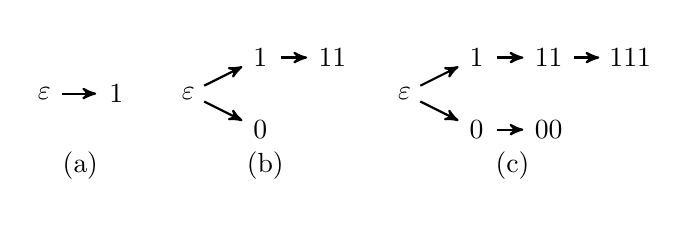
\begin{tikzpicture}[->,>=stealth',auto,thick, scale = 0.61,state/.style={circle,inner sep=2pt}]

    % The graph
	\node [state] at (-3,0) (aR) {$\varepsilon$};
	\node [state] at (-1.5,0) (a1) {$1$};
	\node [state] at (-2.25,-1.5) {(a)};

	% Graph edges
	\path[->]
	(aR) edge (a1);  	

    % The graph
	\node [state] at (0,0) (bR) {$\varepsilon$};
	\node [state] at (1.5,0.75) (b1) {$1$};
	\node [state] at (1.5,-0.75) (b0) {$0$};

	\node [state] at (3,0.75) (b11) {$11$};	
	\node [state] at (1.6,-1.5) {(b)};
	
	% Graph edges
	\path[->]
	(bR) edge (b0)
	(bR) edge (b1)
	(b1) edge (b11);

    % The graph
	\node [state] at (4.5,0) (cR) {$\varepsilon$};
	\node [state] at (6,0.75) (c1) {$1$};
	\node [state] at (6,-0.75) (c0) {$0$};

	\node [state] at (7.5,-0.75) (c00) {$00$};
	
	\node [state] at (7.5,0.75) (c11) {$11$};	
	\node [state] at (9.2,0.75) (c111) {$111$};	
	\node [state] at (6.75,-1.5) {(c)};
	
	% Graph edges
	\path[->]
	(cR) edge (c0)
	(c0) edge (c00)
	(cR) edge (c1)
	(c1) edge (c11)
	(c11) edge (c111);

\end{tikzpicture} 
\end{center}

\caption{States in a game played according to strategy $\baf$. \label{fig:proof-theorem-4}}
\end{figure}

Since all states where player $1$ receives a reward involve putting a block in the blockchain, all words 
$w$ with $r_1(w) > 0$ are therefore of the form $d\cdot 1\cdot w'$ with $d \in \Dyck$. Now let $q$ be the only state such that  $d\cdot 1\cdot w' \in \tau(q)$.
% be the state represented by $d\cdot 1\cdot w'$. 
State $q$ can be seen as a tree with two branches: one only with blocks earned by player $0$, and the other one 
with at least ${\frac{|d|}{2}+1}$ blocks owned by player $1$ (plus maybe more, depending on $w'$). 
We can then calculate the reward for $q$ as $r_1(q) = r_1(d \cdot 1) + \alpha^{\frac{|d|}{2}+1}\cdot r_1(w')$, obtaining that:
%\begin{eqnarray*}
%%r_1(q) & = & \bigg(\sum_{i=1}^{\frac{|d|}{2}+1}\alpha^i \bigg)+ \alpha^{\frac{|d|}{2}+1}\cdot r_1(w').
%r_1(q) & = & r_1(d \cdot 1) + \alpha^{\frac{|d|}{2}+1}\cdot r_1(w').
%\end{eqnarray*}
%Hence, we obtain $u_1(\baf)$ is equal to:
\begin{multline*}
u_1(\baf) \ = \ (1-\beta) \cdot \sum_{d\in \Dyck}  \sum_{w\in \{0,1\}^*} \bigg(\beta^{|d|+1+|w|}\cdot \\
 \big[r_1(d\cdot 1) + \alpha^{\frac{|d|}{2}+1}\cdot r_1(w)\big] \cdot \pr(d\cdot 1 \cdot w)\bigg).
\end{multline*}
%
%The product of probabilities is obtained since winning a block is an independent trial. 
Splitting up the summation, we get that $ u_1(\baf)$ is equal to:
\begin{align*}
&(1-\beta) \cdot \sum_{d\in \Dyck}  \sum_{w\in \{0,1\}^*}\beta^{|d|+1+|w|}\cdot r_1(d\cdot 1) \cdot \pr(d\cdot 1\cdot w) \ +\\
 & (1-\beta) \cdot \sum_{d\in \Dyck}  \sum_{w\in \{0,1\}^*}\beta^{|d|+1+|w|}\cdot  \alpha^{\frac{|d|}{2}+1}\cdot r_1(w) \cdot \pr(d\cdot 1 \cdot w).
\end{align*}
%
We denote the first term in the equation above by $\Phi$. 
By definition of the probability of a word, we have that $\pr(d\cdot 1\cdot w) = \pr(d\cdot 1)\cdot \pr(w)$. 
Next, we use this fact in the expression for $u_1(\baf)$ to split the second term into the elements that depend only on $d$, and the ones that depend only on $w$:
%
\begin{multline*}
 u_1(\baf) \ = \Phi  \ +  \bigg(\sum_{d\in \Dyck} \beta^{|d|+1}\cdot  \alpha^{\frac{|d|}{2}+1}\cdot \pr(d\cdot 1)\bigg) \cdot \\
 \bigg((1-\beta) \cdot \sum_{w\in \{0,1\}^*} \beta^{|w|} \cdot r_1(w)  \cdot \pr(w)\bigg).
\end{multline*}
%
Since the term $(1-\beta) \cdot \sum_{w\in \{0,1\}^*} \beta^{|w|} \cdot r_1(w)  \cdot \pr(w)$ is precisely $u_1(\baf)$, we have that:
%
\begin{eqnarray*}
 u_1(\baf) & = & \Phi + 
 \bigg(\sum_{d\in \Dyck} \beta^{|d|+1}\cdot  \alpha^{\frac{|d|}{2}+1}\cdot \pr(d\cdot 1)\bigg) \cdot  u_1(\baf).
\end{eqnarray*}
%
By denoting with $\Gamma$ the term $\sum_{d\in \Dyck} \beta^{|d|+1}\cdot  \alpha^{\frac{|d|}{2}+1}\cdot \pr(d\cdot 1)$, we get the equation
$u_1(\baf) = \frac{\Phi}{1-\Gamma}$.
%\begin{eqnarray*}
%u_1(\baf) & = &  \frac{\Phi}{1-\Gamma}.
%\end{eqnarray*}
Let us now find a closed form for~$\Gamma$:
%. In what follows, we use $\Dyck_{2\ell}$ to denote the set of all Dyck words of length $2\ell$ (recall that all Dyck words are of even length):
%
\begin{eqnarray*}
\Gamma & = & \sum_{d\in \Dyck} \beta^{|d|+1}\cdot  \alpha^{\frac{|d|}{2}+1}\cdot \pr(d\cdot 1)\\
% & = & \alpha\cdot \beta \cdot  \sum_{d\in \Dyck} \beta^{|d|}\cdot  \alpha^{\frac{|d|}{2}}\cdot \pr(d\cdot 1) \\
  & = & \alpha\cdot \beta \cdot \sum_{\ell = 0}^{\infty} \sum_{d\in \Dyck_{2\ell}} (\alpha\cdot \beta^2)^{\ell}\cdot h^{\ell}\cdot (1-h)^{\ell}\cdot h\\
%   & = &  \alpha\cdot \beta \cdot \sum_{\ell = 0}^{\infty} |\Dyck_{2\ell}| \cdot (\alpha\cdot \beta^2)^{\ell}\cdot h^{\ell}\cdot (1-h)^{\ell}\cdot h\\
      & = &  \alpha\cdot \beta \cdot h \cdot \sum_{\ell = 0}^{\infty} |\Dyck_{2\ell}| \cdot (\alpha\cdot \beta^2 \cdot h \cdot (1-h))^{\ell}\\
    & = &  \alpha\cdot \beta \cdot h \cdot \cat(\alpha\cdot\beta^2 \cdot h \cdot (1-h)).
\end{eqnarray*}
%
%Here the third equality follows since all Dyck words are of even length (we use $\Dyck_{2\ell}$ to denote the set of all Dyck words of length $2\ell$). 
The final equality is obtained by recalling the fact that $|\Dyck_{2\ell}|$ is the $\ell$-th Catalan number, so that the summation in the previous line defines the generating function of these numbers. Notice that function $\cat(x)$ is defined and continuous for $x \in (0,\frac{1}{4}]$, and that $\alpha\cdot\beta^2 \cdot h \cdot (1-h) \in (0,\frac{1}{4}] $ since $\alpha \in (0,1]$, $\beta \in (0,1)$ and $h\cdot(1-h)\in (0,\frac{1}{4})$ for every $h\in(0,1)$.

The closed form for $\Phi$ is computed analogously, yielding the claimed expression.
\end{proof}



%%%OFF :) THE VERSION JUAN HAD BEFORE MY PASS
\begin{comment}
\begin{proof}
Let $Q_\baf = \{q \in \bQ \mid \pr^\baf(q) > 0\}$ be the set of all states that can be reached from the genesis using strategy $\baf$, and recall 
the mapping $\sigma: Q_\baf \rightarrow \{0,1\}^*$ introduced  in the proof of Theorem \ref{thm-conts_dom_str}, now in the context of strategy $\baf$. From the definition of $\sigma$ we have that for any state $q \in Q_\baf$ one verifies 
$\pr^{\baf}(q \mid \varepsilon) = \sum_{w \in \sigma(q)} \pr(w \mid \varepsilon)$, where $\pr(w \mid \varepsilon)$ for a word $w$ with $n_0$ zeroes and $n_1$ ones is simply 
$h^{n_1}(1-h)^{n_0}$. Further, by Claim \ref{claim-nonempty-inter-gen} the inverse  $\sigma^{-1}: \{0,1\}^* \rightarrow Q_\baf$ is a total function.  
All of this means that we can rewrite the utility of player $1$ using $\baf$ as: 
\begin{multline*}
u_1(\baf \mid \varepsilon) = \sum_{q \in \bQ} \beta^{|q|-1} \cdot  r_1(q) \cdot \pr^{\cdf}(q \mid \varepsilon) = \\ 
\sum_{q \in \bQ} \sum_{w \in \sigma(q)} \beta^{|w|} \cdot  r_1(w) \cdot \pr(w \mid \varepsilon) =  \\
\sum_{w \in \{0,1\}^*} \beta^{|w|} \cdot  r_1(w) \cdot \pr^{\baf}(w \mid \varepsilon),
\end{multline*}
where $r_1(w)$ is just a convenient shorthand for $r_1(\sigma^{-1}(w))$.


%Since $\varepsilon\subseteq q$, for any state $q\in \bQ$, by the definition of utility we have that: 

%$$u_1(\baf\mid\varepsilon) = \sum_{q\in \bQ}\beta^{|q|}\cdot r(q)\cdot \pr^{\baf}(q\mid \varepsilon).$$

%Applying the idea of coding the states in a two player game as sequences of binary numbers, we can write the above as:

%\begin{equation}\label{eq:def_utility}
%u_1(\baf\mid\varepsilon) = \sum_{w\in \{0,1\}^*}\beta^{|w|}\cdot r(w)\cdot \pr^{\baf}(w\mid \varepsilon).
%\end{equation}

Now, let us consider the set $S$ of all words $w \in \{0,1\}^*$ that represent states $q$ (via $\sigma$) in which player $1$ owns at least one block in the blockchain for the first time. 
The easiest of them is $w = 1$, which represents the state in Figure XXX. This state is created when player $q$ wins the first move of the game, sucesfully mining upon the genesis block. Next is word $011$, representing the state in Figure YY. To arrive at this state player $0$ must have mined the first block, player $1$ forked and then player $1$ 
forked again. The next words in $S$ are $00111$ and $01011$, both representing the state of Figure ZZZ. 
In general, the words in the set $S$ have the form $d1$, where $d$ is a \emph{Dyck word}: a word with the same number of $0$s and $1$s, but such that 
no prefix of $d$ has more $1$s than $0$s (this intuitively signifies that player $1$ never had more blocks than $0$ at any point). 
Note that the only dyck word of length $0$ is $\epsilon$, the next dyck word by length is $01$, and then $0011$ and $0101$. 

\begin{figure}
\begin{subfigure}{0.2\columnwidth}
\begin{tikzpicture}[->,>=stealth',auto,thick, scale = 1.0,state/.style={circle,inner sep=2pt}]

    % The graph
	\node [state] at (-2,0) (R) {$\varepsilon$};
	\node [state] at (-0.5,0) (1) {$1$};

	% Graph edges
	\path[->]
	(R) edge (1);  	
\end{tikzpicture} 
\end{subfigure} 
\qquad
\begin{subfigure}{0.3\columnwidth}
\begin{tikzpicture}[->,>=stealth',auto,thick, scale = 1.0,state/.style={circle,inner sep=2pt}]

    % The graph
	\node [state] at (0,0) (R) {$\varepsilon$};
	\node [state] at (1.5,0.75) (1) {$1$};
	\node [state] at (1.5,-0.75) (0) {$0$};

	\node [state] at (3,0.75) (11) {$11$};	
	
	% Graph edges
	\path[->]
	(R) edge (0);  	
	
	\path[->]
	(R) edge (1)
	(1) edge (11);

\end{tikzpicture} 
\end{subfigure}

\begin{subfigure}[b]{0.3\textwidth}
\begin{center}
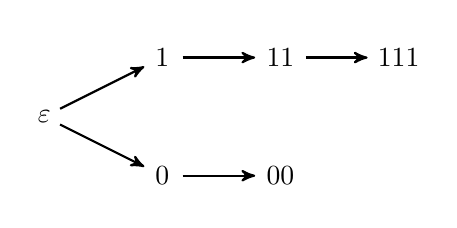
\begin{tikzpicture}[->,>=stealth',auto,thick, scale = 1.0,state/.style={circle,inner sep=2pt}]

    % The graph
	\node [state] at (0,0) (R) {$\varepsilon$};
	\node [state] at (1.5,0.75) (1) {$1$};
	\node [state] at (1.5,-0.75) (0) {$0$};

	\node [state] at (3,-0.75) (00) {$00$};
	
	\node [state] at (3,0.75) (11) {$11$};	
	\node [state] at (4.5,0.75) (111) {$111$};	
	
	% Graph edges
	\path[->]
	(R) edge (0)
	(0) edge (00);  	
	
	\path[->]
	(R) edge (1)
	(1) edge (11)
	(11) edge (111);

\end{tikzpicture} 
\end{center}
\end{subfigure}

\caption{XXX}
\label{fig:proof-theorem-4}
\end{figure}

Since all states where player $1$ receives a reward involve putting a block in the blockchain, all words 
$w$ with $r_1(w) > 0$ are therefore of the form $d 1 w'$. Now let $q = \sigma^{-1}(d1w')$ be the state represented by $d1w'$. 
State $q$ can be seen as a tree with two branches: one only with blocks earned by player $0$, and the other one 
with at least ${\frac{|d|}{2}+1}$ blocks owned by player $1$ (plus maybe more, depending on $w$). 
We can then calculate the reward for $q$: 
$$r_1(q) = \big(\sum_{i=1}^{\frac{|d|}{2}+1}\alpha^i \big)+ \alpha^{\frac{|d|}{2}+1}\cdot r_1(\sigma^{-1}(w)).$$
Therefore (and writing $r_1(w)$ for $r_(\sigma^{-1}(w)))$, we can write:
%
%Now notice that when playing $\baf$, player 1 will fork each time she loses a block. This in particular means, that the states where she will receive an award for her blocks will always start with her winning one or more forks. For instance, in Figure \ref{fig:always_fork}, player 1 receives an award in block 11, which corresponds to a state coded by the word $w=011$. A similar story holds true for block 111, which corresponds to a state coded by the word $w=01101$. In general, states where player 1 receives an award can be coded by a Dyck word $d$, where both 1 and 0 have the same number of blocks in the game, followed by a block won by 1. After that any word $w$ can follow, leaving us in a state coded by $d1w$. Notice that the reward of player 1 in this state can be split into the reward for $d1$ (since this will always be part of $\meet(q)$, for $q$ the state corresponding to $d1w$), and the reward for $w$, with a shift of $\alpha^{\frac{|d|}{2}+1}$, since the latter is the length of the longest common chain before $w$ starts. Therefore, we can write the above utility as follows:
%
\begin{eqnarray*}
u_1(\baf\mid\varepsilon) = \sum_{d\in \dyck}  \sum_{w\in \{0,1\}^*}\beta^{|d|+1+|w|}\cdot \big[r(d1) + \alpha^{\frac{|d|}{2}+1}\cdot r(w)\big] \cdot \\ \pr^{\baf}(d1\mid \varepsilon)\cdot \pr^{\baf}(w\mid \varepsilon).
\end{eqnarray*}
%
The product of probabilities is obtained since winning a block is an independent trial. Splitting up the sums we get:
\begin{align*}
 & u_1(\baf\mid\varepsilon) = \\
 & \sum_{d\in \dyck}  \sum_{w\in \{0,1\}^*}\beta^{|d|+1+|w|}\cdot r(d1) \cdot \pr^{\baf}(d1\mid \varepsilon)\cdot \pr^{\baf}(w\mid \varepsilon)
 \mbox{ } +\\
 & \sum_{d\in \dyck}  \sum_{w\in \{0,1\}^*}\beta^{|d|+1+|w|}\cdot  \alpha^{\frac{|d|}{2}+1}\cdot r(w) \cdot \pr^{\baf}(d1\mid \varepsilon)\cdot \pr^{\baf}(w\mid \varepsilon).
\end{align*}
%
We will denote the first term in the equation above by $\varphi$. 
%
%More precisely,
%$$\varphi = \sum_{d\in \dyck}  \sum_{w\in \{0,1\}^*}\beta^{|d|+1+|w|}\cdot r(d1) \cdot \pr^{\baf}(d1\mid \varepsilon)\cdot \pr^{\baf}(w\mid \varepsilon).$$

Next, in the expression for $u_1(\baf\mid\varepsilon)$ we will split the second term into the elements that depend only on $d$, and the ones that depend only on $w$, getting:
%
\begin{align*}
 & u_1(\baf\mid\varepsilon) = \varphi \mbox{ } +\\
 & \sum_{d\in \dyck} \beta^{|d|+1}\cdot  \alpha^{\frac{|d|}{2}+1}\cdot \pr^{\baf}(d1\mid \varepsilon) \cdot 
 \sum_{w\in \{0,1\}^*} \beta^{|w|} \cdot r(w)  \cdot \pr^{\baf}(w\mid \varepsilon).
\end{align*}
%
But the rightmost sum is precisely $u_1(\baf\mid\varepsilon)$. Thus, 
%
\begin{align*}
 u_1(\baf\mid\varepsilon) = \varphi \mbox{ } + 
 \sum_{d\in \dyck} \beta^{|d|+1}\cdot  \alpha^{\frac{|d|}{2}+1}\cdot \pr^{\baf}(d1\mid \varepsilon) \cdot  u_1(\baf\mid\varepsilon).
\end{align*}
%
We denoting by $\Gamma$ the rightmost term of the sum above we get the equation:
$$u_1(\baf\mid\varepsilon) = \frac{\varphi}{1-\Gamma}.$$
Let us now find a closed form for $\Gamma$.
%
\begin{align*}
\Gamma = & \sum_{d\in \dyck} \beta^{|d|+1}\cdot  \alpha^{\frac{|d|}{2}+1}\cdot \pr^{\baf}(d1\mid \varepsilon)\\
 = & \mbox{ } \alpha\cdot \beta \sum_{d\in \dyck} \beta^{|d|}\cdot  \alpha^{\frac{|d|}{2}}\cdot \pr^{\baf}(d1\mid \varepsilon) \\
  = & \mbox{ } \alpha\cdot \beta \sum_{\ell = 0}^{\infty} \sum_{d\in \dyck_{2\ell}} (\alpha\cdot \beta^2)^{\ell}\cdot h^{\ell}\cdot (1-h)^{\ell}\cdot h\\
   = & \mbox{ } \alpha\cdot \beta \sum_{\ell = 0}^{\infty} |\dyck_{2\ell}| (\alpha\cdot \beta^2)^{\ell}\cdot h^{\ell}\cdot (1-h)^{\ell}\cdot h\\
    = & \mbox{ } \alpha\cdot \beta \cdot h \cdot Cat(\alpha\cdot\beta^2 \cdot h \cdot (1-h)).\\
\end{align*}
%
Here the third equality follows since all Dyck words are of even length. The final equality is obtained using the fact that the $\ell$th Catalan number is equal to the number of Dyck words of length $2\ell$, thus the summation in the previous line defines the generating function of Catalan numbers.

The closed form for $\varphi$ is computed in a similar way, constructing again generating functions of catalan numbers of specific parameters. 
\end{proof}
\end{comment}

\medskip
\noindent
\textbf{When to fork}. To answer this question, we used the closed forms of $\bdf$ and $\baf$ to compute the utility for a fixed $\alpha$, $\beta$ and varying hash power. 
We consider reallistic values of $\alpha$ and $\beta$ as follows. For $\alpha$ we calculate the compound version of the discount in Bitcoin, that is, 
a value of alpha that would divide the reward by half every 210.000 blocks, \ie $\alpha = 0.9999967030$. For 
$\beta$ we calculate the 10-minute rate that is equivalent to the US real interest rate in 2017 \cite{interest}, which amounts to 2.2077\%. This gives us a value of $\beta = 0.9999996156$. 

Figure \ref{fig-af-df-fo} shows the value of the utility for player $1$ when using strategies $\af$, $\pf{1}$ or $\df$, and player $0$ always using $\df$. The point where the utility for 
$\af$ and $\df$ meet is $h = 0.4969 \pm 0.000001$ \francisco{Confirmed with the c++ scripts with thousands of bits of precision actually}, which means that player $1$ should use $\af$ as soon as she controls more than this proportion of the hash power. This confirms the 
folklore fact that is profitable to fork with more than half the hash power. However, it is interesting to note that this is not exactly the case: one should be willing to fork even with a little less than half the hash power. This has been noted before in e.g. \cite{}. \francisco{Should we mention that this is quite expectable from the strategies? i.e. the probability of being ahead at one point in time is almost one for $h > .4969$, so it is actually not very interesting.}

\begin{figure}
  \centering
    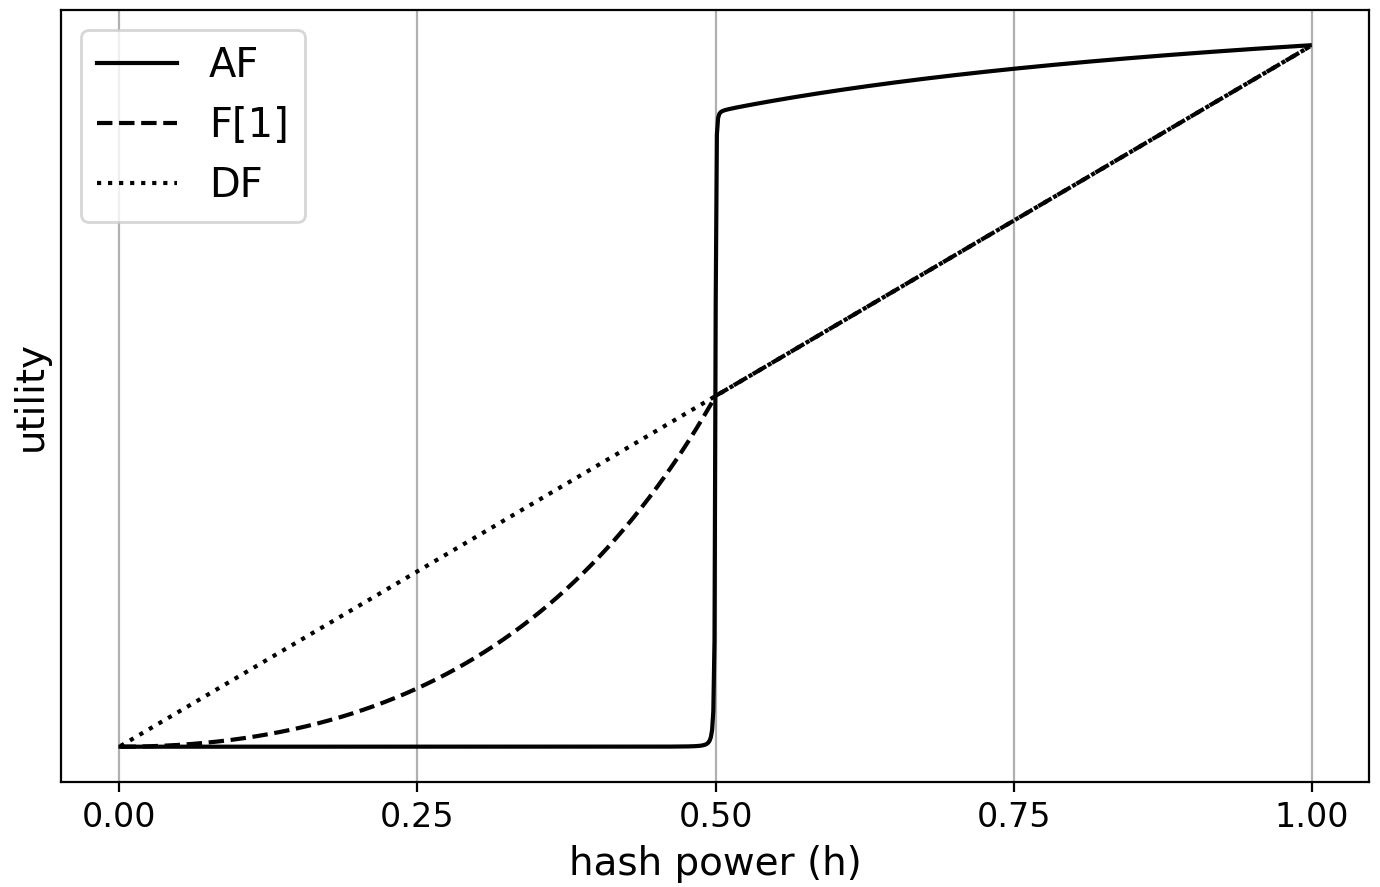
\includegraphics[width=0.46\textwidth]{plots/test_AF.png}
    \caption{Utility for player $1$ under strategies $\bdf$, $(\df_0,\pf{1})$ and $\baf$. The curve for $\pf{1}$ is too close to that of $\df$ to tell a difference at this scale, but the difference does exist: after about $h = 0.5$, the curve for $\pf{1}$ is always higher than that of $\df$. Note that the utility collapses to $\df$ when $h = 1$. This is always the highest amount that can be earned in our game.}
        \label{fig-af-df-fo}
\end{figure}

\smallskip
\noindent
\francisco{I think the following subsection should not be included (or should be restated as only considering AF vs DF). The comparation with F[i] looks quite weak to me.}
\textbf{Forking for a fixed number of times}. Looking at Figure \ref{fig-af-df-fo}, we see that the utility when using $\pf{1}$ is  between the lines for $\af$ and $\df$. 
This utility was calculated using a similar strategy as in in the proof of Theorem \ref{thm:always_fork}. 
From the figure one can infer that, assuming $\af$ yields more utility to player $1$ than $\df$ (e.g. when $h>0.5$), then player $1$ should not use $\pf{1}$ but rather keep on forking, as 
the utility for $\af$ is always above than the utility for $\pf{i}$ in that case. %Can we say the same for other similar strategies? Even though we can compute the utility of using any of the strategies $\pf{i}$, we cannot directly compare an infinite number of strategies. Instead, we prove the following general result. 
We can show something similar for all the other $\pf{i}$.
\begin{proposition}\label{prop-fork_fix}
Assume that $u_1(\bdf) \leq u_1(\baf)$ for some $\alpha,\beta,h$. Then for all $i > 0$ we have that $u_1((\df_0,\pf{i})) \leq u_1(\af))$.
\end{proposition}

Note that this result does not rule out the possibility that, for some amount of hash power, playing some $\pf{i}$ would turn out better than $\df$, but $\af$ would not. We know 
this is not the case for $i = 1$, and we can also prove it for $i > 1$, albeit at the cost of much more powerful machinery that we do not have the space to introduce. 
However, in the following section we do show that there are actually strategies leading to forks with less hash power. 

\subsection{Giving up for more utility}

By adding a little more flexibility to the strategy of always forking we can identify strategies that make forking profitable with less hash power. 

The families of strategies that we study in this section involve two parameters. First, a \textit{give-up} parameter $\ell$ that mandates the maximum length of the fight the miner is willing to put when forking, and a parameter $k$ that regulates how far back does the miner fork, when confronted with a chain of blocks I don't own. We denote these strategies by $\gup_\ell^k$. Both parameters can be seen as a refinement of the way $\af$ works, and indeed $\af$ would be equivalent to the strategy $\gup_\infty^\infty$ where player $1$ is willing to keep fights of any length and to fork at the beginning of any chain of blocks she does not own.  

\begin{figure}
\begin{center}
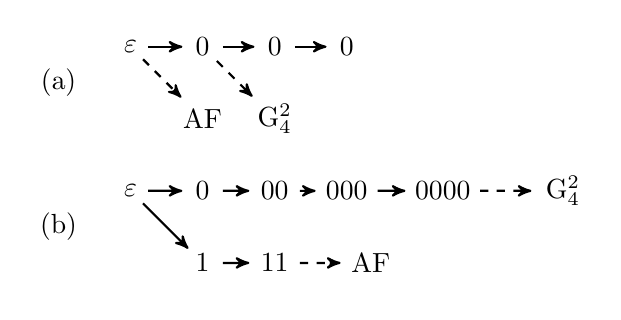
\begin{tikzpicture}[->,>=stealth',auto,thick, scale = 0.61,state/.style={circle,inner sep=2pt}]

    % The graph
	\node [state] at (-10.5,0) (aR) {$\varepsilon$};
	\node [state] at (-9,0) (a0) {$0$};
	\node [state] at (-7.5,0) (a00) {$0$};
	\node [state] at (-6,0) (a000) {$0$};
	\node [state] at (-9,-1.5) (aAF) {$\af$};
	\node [state] at (-7.5,-1.5) (aG) {$\gup_4^2$};
	\node [state] at (-12,-0.75) {(a)};

	% Graph edges
	\path[->]
	(aR) edge (a0)
	(a0) edge (a00)
	(a00) edge (a000);
  	
	\path[->,dashed]
	(aR) edge (aAF)
	(a0) edge (aG);
	
    % The graph
	\node [state] at (-10.5,-3) (bR) {$\varepsilon$};
	\node [state] at (-9,-3) (b0) {$0$};
	\node [state] at (-7.5,-3) (b00) {$00$};
	\node [state] at (-6,-3) (b000) {$000$};
	\node [state] at (-4,-3) (b0000) {$0000$};
	\node [state] at (-9,-4.5) (b1) {$1$};
	\node [state] at (-7.5,-4.5) (b11) {$11$};
	\node [state] at (-5.5,-4.5) (bAF) {$\af$};
	\node [state] at (-1.5,-3) (bG) {$\gup_4^2$};
	\node [state] at (-12,-3.75) {(b)};

	% Graph edges
	\path[->]
	(bR) edge (b0)
	(bR) edge (b1)
	(b1) edge (b11)
	(b0) edge (b00)
	(b00) edge (b000)
	(b000) edge (b0000);
  	
	\path[->,dashed]
	(b11) edge (bAF)
	(b0000) edge (bG);
	

\end{tikzpicture} 
\end{center}

\caption{Difference between $\af$ and $\gup^2_4$ in terms of actions of these strategies in two states. In (a), the value $k = 2$ indicates that $\gup^2_4$ will not 
fork on $\varepsilon$ but instead in $0$. In (b), the value $\ell = 4$ indicates that in this state player $1$ should give up the fork and continue mining upon the blockchain (block $0000$)}
\label{fig-gup}
\end{figure}

\begin{example}
Let us consider how $\gup_4^2$ would be different from $\af$. Since $k = 2$, both strategies take the same action when confronted to chains of zero, one or two blocks owned by player $0$, namely, mining at $\varepsilon$. Hence, assume that both strategies are facing a chain of three unowned new blocks in the blockchain, as in Figure \ref{fig-gup}-a. In this case, $\af$ would again try to fork from her own block, but $\gup_4^2$ would fork instead on the dotted line (i.e., the $k$-th unowned block).
The second difference is provided by the give-up time (Figure \ref{fig-gup}-b). Normally, $\af$ is willing to continue forking regardless of winning hopes, therefore the move for state $q'$ in Figure \ref{fig-gup}-b would still be to mine upon her own block $11$. On the other hand $\gup_4^2$ has already seen $4$ blocks from the start of the fork, so with this strategy player $1$ instead gives up and tries to mine upon $0000$, rebooting the strategies as if this last block was the genesis block. 
\end{example}

To compute an analytical form for $u_1(\gup_\ell^k)$ we proceed as in the proof of Theorem \ref{thm:always_fork}. In this case, the set of paths leading to winning states has a more complex combinatorial nature, as expected when taking into account the disadvantage and give-up parameters $k,\ell$. We obtain the following.

\begin{theorem}
For every pair of positive integers $\ell, k$ with $k<l$, we have 
$$u_1(\bgup^k_\ell) = \frac{\varphi_{\tiny l,k}}{1-\Gamma_{l,k}},$$
where $\varphi_{l,k}$ and $\Gamma_{l,k}$ are polynomials in $\alpha$, $\beta$ and $h$. 
\end{theorem}

In other words, given specific $k$ and $\ell$, we can still compute the utility of these strategies. We use this theorem to analyse these strategies, plotting them as we did before, 
for $\alpha = 0.9999967030$ and $\beta = 0.9999996156$. Figure \ref{fig-plot-gup-fixwindow} gives us an interesting feel for the advantages of this family of strategies. 
We fix $k = 1$, and plot the utility of strategies $\bgup^1_2$ through $\bgup^1_5$, and we shaded those areas in which one of the utilities is greater. As wee see, for a 
fork window $k = 1$, the optimal amount time player $1$ should be willing to fight a fork before giving up depends on the hash power. With little hash power the likelihood of winning a 
fork is small, so we want to give up as early as possible. However, the more hash power we obtain, the better it is to wait more and more. Interestingly, with a little more than 
$46\%$ of the hash power player $1$ already should start using strategies $\gup^1_4$ and with a little more power, $\gup^1_5$. We know that player $1$ should use $\af$ not before 
$h = 0.499$, so this gives us a loot of extra room to look for optimal strategies if we are willing to fork (especially considering every percentage of hash power in popular cryptocurrencies 
may cost millions).

\begin{figure}
  \centering
    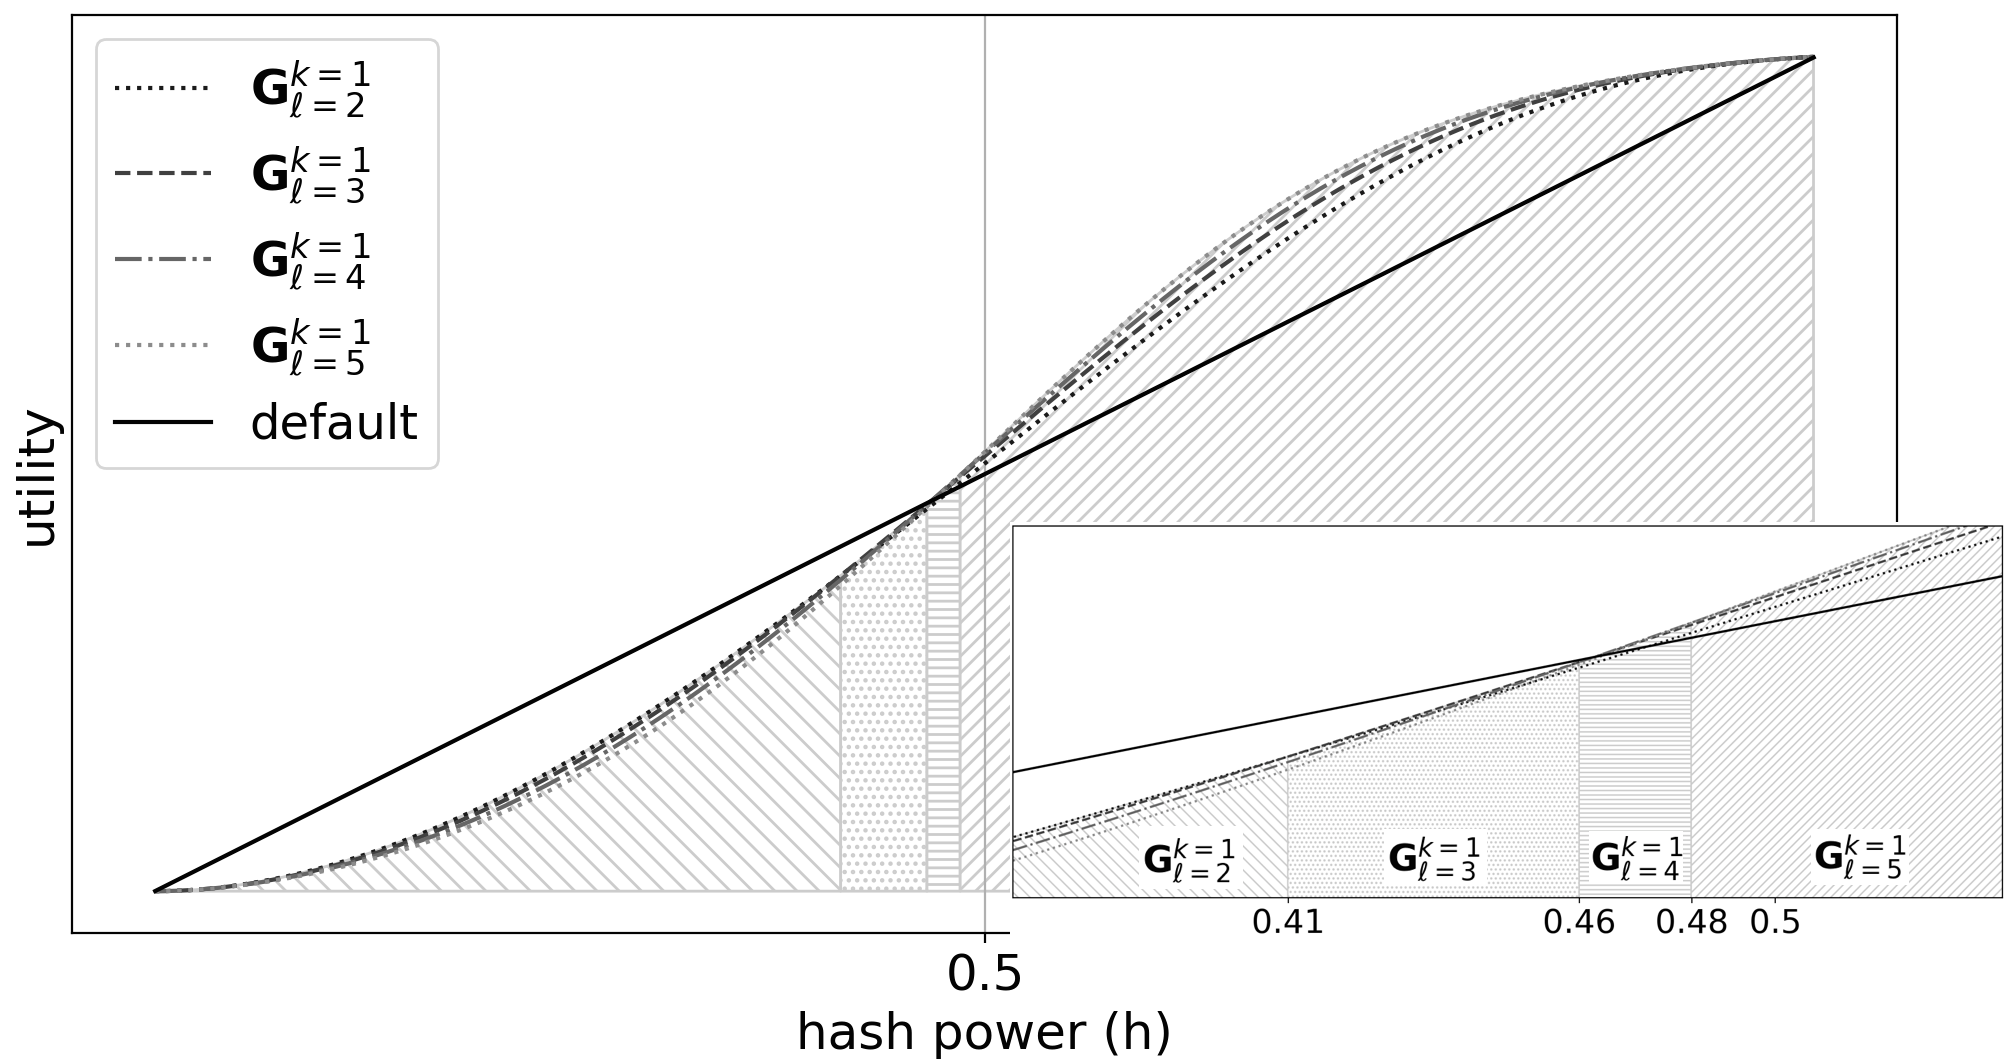
\includegraphics[width=0.46\textwidth]{plots/GUP.png}
    \label{fig-plot-gup-fixwindow}
    \caption{Utility for player $1$ under strategies $\bgup^1_2, \dots, \bgup^1_5$. Shaded areas indicate which strategy yields higher utility at a given hash power. 
    The rightmost box represents a zoom around $h = 0.4$ and $h = 0.5$, and the curve for $\bgup^1_4$ meets that of $\bdf$ at $h = 0.467$. All data was generated with arbitrary floating point precision (GMP).}
\end{figure}

Plots for strategies with $k > 1$ present a similar behaviour: the more hash power we have, the more we should be willing to fight our forks. However, 
Figure \ref{fig-plot-gup-fixwindow} is important because we have found that strategy $\gup^1_4$ is the strategy that beats default under the least amount of hash power 
amongst any combination of $k$, $\ell$. The comparison is much less straightforward when looking at varying values of both $k$ and $\ell$, but in general, 
the more hash power the bigger the window of blocks one should aim to fork, and the more time one should wait before giving up. We remark that the analysis 
we can do through 2- or 3-dimensional plots is only one part of the picture, and that a game-thoretical analysis of these strategies is an interesting area for future work. 


%%%%%%%%%%%%%%%%%%%%%%%%%%%%%%%%%%%%%%%%%%%%%%%%%%%%%%%%%%%%%%%%%%%%%%%%%
%%% BELOW IS THE PREVIOUS VERSION THAT I STILL DID NOT MAKE A PASS ON %%%
%%%%%%%%%%%%%%%%%%%%%%%%%%%%%%%%%%%%%%%%%%%%%%%%%%%%%%%%%%%%%%%%%%%%%%%%%

\begin{comment}

\paragraph{Forking in the genesis block.}
The first forking strategy we models the case when 0 has won the ultimate block. The question 1 wants to answer in this situation is whether she should continue mining on the blockchain, playing according to $\df$, or should she fork, mining instead upon her previously won block? Since by the proof of Theorem \ref{thm-conts_equlibria} we know that optimal strategies for 1 depend only on the blocks following her last block in each state, we can focus on this question when the game is just starting, that is, when 1 wants to decide whether to fork in the genesis block. We will denote by $\fg_1$ the strategy in which player 1 is trying to win the first block following genesis, and once this branch becomes the new blockchain, continues mining using the default strategy. We denote by $\fg = (\df_0,\fg_1)$ the strategy where 1 tries to win the first block in the final blockchain, and 0 mines using the default strategy. A depiction of this strategy is given in Figure \ref{fig-fork_genesis}. When player 1 uses this strategy, we can compute her utility as follows.

\begin{figure}
\begin{center}
\begin{tikzpicture}[->,>=stealth',auto,thick, scale = 1.0,state/.style={circle,inner sep=2pt}]

    % The graph
	\node [state] at (0,0) (R) {$\varepsilon$};
	\node [state] at (1.5,0.75) (1) {$1$};
	\node [state] at (1.5,-0.75) (0) {$0$};
	\node [state] at (3,-0.75) (00) {$00$};
	
	\node [state] at (3,0.75) (11) {$11$};		
	\node [state] at (4.6,0.75) (111) {$111$};
	\node [state] at (6.4,0.75) (1110) {$1110$};
			

	
	% Graph edges
	\path[->]
	(R) edge (1)
	(R) edge (0)
	(0) edge (00)
	;  	
	
	\path[->,dashed]
	(1) edge (11)
	(11) edge (111)
	(111) edge (1110)
	;


\end{tikzpicture} 
\end{center}
\caption{Following the block 00 player 1 tries to win a fork starting at $\varepsilon$. Dashed edges show the case in which she succeeds, after which both players mine on top of the new blockchain.}
\label{fig-fork_genesis}
\end{figure}

\begin{myprop}
%	\label{prop-utilityofgenesisinfinite}
	\label{prop:utility_gen_fork}
%	Suppose player 1 plays with the genesis fork strategy and player 0 follows the default strategy. 
Let $h$ be the hash power of player 1. Then
	\begin{eqnarray*}
		u_1^\infty(\fg\mid\varepsilon) =K_1\cdot \Cat(\beta^2h(1-h))+K_2\cdot \Cat(\alpha\beta^2h(1-h))
	\end{eqnarray*}
where $\Cat:x\mapsto \frac{1-\sqrt{1-4x}}{2x}$ is the generating function of Catalan numbers \cite{ADD_CITATION}, and 
	\begin{eqnarray*}
		K_1 =\frac{\alpha\beta h}{(1-\alpha)(1-\beta)},\quad	K_2 =\frac{\alpha^2\beta h(\alpha\beta+h\beta-h\alpha\beta-1)}{(1-\alpha)(1-\beta)(1-\alpha\beta)}.	
	\end{eqnarray*}
\end{myprop}

The intuition behind the appearance of Catalan numbers in this result is that for each fixed $n$, the number of states where two chains of length $n$ are being tied for blockchain equals the $n$th Catalan number (more precisely, they correspond to Dyck paths of length $n$). Since such states dictate when 1 will win the desired fork, and no reward can be won by 1 before this occurs (note that the two branches in this game have only $\varepsilon$ in common), they tell us what the utility of player 1 will be. Notice that since $\beta \leq 1$, and the maximum of the function $h\mapsto h(1-h)$ is $\frac{1}{4}$, for $h\in [0,1]$, the value $Cat(\beta^2h(1-h))$ is always well defined. For the sake of completion, in Appendix \ref{appendix-gen_fork}, we also show what is the utility of $\fg$ for player 1 at each step $n$ of the mining game.

\paragraph{Forking $m$ blocks from the end of the blockchain.} The second forking strategy we consider works similarly as $\fg$, but now player 1 considers forking after losing $m$ consecutive blocks, for some fixed $m$. In this case, 1 will fork $m$ blocks from the end of the current blockchain, all of these $m$ block being owned by 0. This situation is depicted in Figure \ref{fig-fork_m}. Once player 1 wins the fork, and this branch becomes the new blockchain, she will continue mining according to $\df_1$. We denote this strategy of player 1 by $\forkm{m}_1$, and denote with $\forkm{m}=(\df_0,\forkm{m}_1)$ the strategy where 1 uses $\forkm{m}_1$, and 0 plays according to the default strategy.

\begin{figure}
\begin{center}
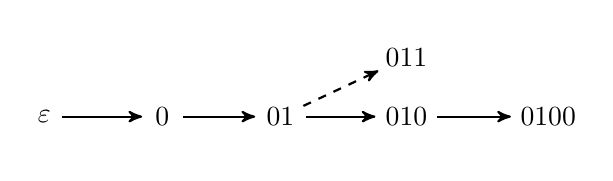
\begin{tikzpicture}[->,>=stealth',auto,thick, scale = 1.0,state/.style={circle,inner sep=2pt}]

    % The graph
	\node [state] at (0,0) (R) {$\varepsilon$};
	\node [state] at (1.5,0) (0) {$0$};
	\node [state] at (3,0) (01) {$01$};
	\node [state] at (4.6,0) (010) {$010$};
	\node [state] at (6.4,0) (0100) {$0100$};
	
	\node [state] at (4.6,0.75) (011) {$011$};					
	
	% Graph edges
	\path[->]
	(R) edge (0)
	(0) edge (01)
	(01) edge (010)
	(010) edge (0100)	
	;  	
	
	\path[->,dashed]
	(01) edge (011)
	;


\end{tikzpicture} 
\end{center}
\caption{If playing $\forkm{2}_1$, player 1 will try to fork after losing two consecutive blocks at position 0100. Should she manage to make the dashed branch into a blockchain, both her and player 1 continue to mine on this branch using $\df$.}
\label{fig-fork_m}
\end{figure}

When computing the utility of $\forkm{m}$ starting in some state $q_0$, we take into account that player 1 is only interested whether her utility will increase in the case she decides to fork. That is, since the blocks before her fork will always have the same constant contribution to her reward in either branch, we will not count them in the utility. With this in mind, the utility of $\forkm{m}$ starting in the state $q_0$ in which 0 has the ultimate $m$ blocks in the (up to now unique) blockchain is given as follows.

\begin{myprop}\label{prop-fork_m}
	Let $h$ be the hash power of player 1. Then
	\begin{eqnarray*}
		u_1(\mfork|q_0) =\bigg(\frac{\beta h}{\alpha}\bigg)^m K_{1}\Cat(\beta^2h(1-h))^{m+1}+(\beta h)^{m}K_{2}\Cat(\alpha\beta^2h(1-h))^{m+1}
	\end{eqnarray*}
	where $\Cat$ is as in Proposition \ref{prop:utility_gen_fork}, and 

\end{myprop}

As before, Catalan numbers help us account for all states where 1 wins the fork. Of course, now player 1 is starting with a handicap of $m$ steps, so the winning states for 1 will be characterized by staircase walks that stay inside the trapezoid $\{(0,0),(m,0),(m+n,n),(0,n)\}$, for some number $n$. The proof of this proposition is given in Appendix \ref{appendix-fork_m}.

\paragraph{When to fork?} Having the utilities of the two forking strategies, we can now compare them to that of the default strategy in order to answer whether 1 should fork or not. Analysing the curves defined by the game parameters ($\alpha,\beta$ and $h$ for $\fg$, and additionally $m$ for $\forkm{m}$), it can be seen that when $h>50\%$, and $\alpha>\beta$, then it is always convenient for 1 to fork, based on the utility resulting from either $\fg$ or (irrespective of $m$) $\forkm{m}$. This confirms the intuition that the player with the majority of hash power can sway the game in her favour, but we can also see that there are several cases when it is convenient to fork even with much lower hash power. This happens in cases when $\alpha$ is significantly bigger than $\beta$, which can be explained by the fact that ???

\end{comment}


\section{Conclusions}


 
	\bibliographystyle{ACM-Reference-Format}
	\bibliography{bibliography}

	\newpage
	\onecolumn
	\appendix
        %!TEX root = main.tex

\section{Proofs and Intermediate Results}
\subsection{Convergence of the utility function}
\label{sec-conver}

To ensure that the utility function $u_p(\bs \mid q_0)$ is well defined, we impose the restriction that for every payoff function $\bR = (r_0, \ldots, r_{m-1})$, there exists a polynomial $P$ such that $|r_p(q)| \leq P(|q|)$ for every player $p \in \bP$ and state $q \in \bQ$. In this section, we prove that this is indeed a sufficient condition for $u_p(\bs \mid q_0)$ to be a real number, for which we first need a technical lemma. 

\begin{mylem}\label{lem-prop-k}
Let $q_0 \in \bQ$ and $\bs$ be a combined strategy. Then for every $k \geq 0$, it holds that
\begin{eqnarray*}
\sum_{\substack{q \in \bQ \,: \\ q_0 \subseteq q \text{ {\rm and} } |q| - |q_0| = k}} \pr^{\bs}(q \mid q_0) & = & 1.
\end{eqnarray*}
\end{mylem}

\begin{proof}
We prove the lemma by induction on $k$. For $k=0$ the property trivially holds since $\pr^{\bs}(q_0 \mid q_0) = 1$. Thus, assuming that the property holds for $k$, we need to prove that it holds for $k+1$. We have that:
\begin{align*}
&\sum_{\substack{q \in \bQ \,: \\ q_0 \subseteq q \text{ {\rm and} } |q| - |q_0| = k+1}} \pr^{\bs}(q \mid q_0) \ =\\
&\hspace{30pt}\sum_{\substack{q \in \bQ \,: \\ q_0 \subseteq q \text{ {\rm and} } |q| - |q_0| = k+1}} 
\bigg(\sum_{\substack{q' \in \bQ \,: \\ q_0 \subseteq q' \text{ {\rm and} } |q'| - |q_0| = k}} \pr^{\bs}(q' \mid q_0) \cdot \pr(q',\bs(q'),q)\bigg) \ = \\
&\hspace{30pt}\sum_{\substack{q' \in \bQ \,: \\ q_0 \subseteq q' \text{ {\rm and} } |q'| - |q_0| = k}}
\bigg(\sum_{\substack{q \in \bQ \,: \\ q_0 \subseteq q \text{ {\rm and} } |q| - |q_0| = k+1}} 
 \pr^{\bs}(q' \mid q_0) \cdot \pr(q',\bs(q'),q)\bigg) \ =\\
 &\hspace{30pt}\sum_{\substack{q' \in \bQ \,: \\ q_0 \subseteq q' \text{ {\rm and} } |q'| - |q_0| = k}}
\pr^{\bs}(q' \mid q_0) \cdot \bigg(\sum_{\substack{q \in \bQ \,: \\ q_0 \subseteq q \text{ {\rm and} } |q| - |q_0| = k+1}} 
  \pr(q',\bs(q'),q)\bigg) \ =\\
&\hspace{30pt}\sum_{\substack{q' \in \bQ \,: \\ q_0 \subseteq q' \text{ {\rm and} } |q'| - |q_0| = k}}
\pr^{\bs}(q' \mid q_0) \cdot \bigg(\sum_{\substack{q \in \bQ \,: \\ q_0 \subseteq q,\ |q| - |q_0| = k+1,\ \bs(q') = (a_0, \ldots, a_{m-1}) \text{ {\rm and}}\\
\text{{\rm there exists }} p \in \{0, \ldots, m-1\} \text{ {\rm such that} } q = a_p(q')}}
  \pr(q',\bs(q'),q)\bigg) \ =\\
  &\hspace{30pt}\sum_{\substack{q' \in \bQ \,: \\ q_0 \subseteq q' \text{ {\rm and} } |q'| - |q_0| = k}}
\pr^{\bs}(q' \mid q_0) \cdot \bigg(\sum_{\substack{p \in \{0, \ldots, m-1\} \, : \\ \bs(q) = (a_0, \ldots, a_{m-1})}} \pr(q',\bs(q'),a_p(q'))\bigg) \ =\\
&\hspace{30pt}\sum_{\substack{q' \in \bQ \,: \\ q_0 \subseteq q' \text{ {\rm and} } |q'| - |q_0| = k}}
\pr^{\bs}(q' \mid q_0).
\end{align*}
Hence, given that
\begin{eqnarray*}
\sum_{\substack{q' \in \bQ \,: \\ q_0 \subseteq q' \text{ {\rm and} } |q'| - |q_0| = k}}
\pr^{\bs}(q' \mid q_0) & = & 1
\end{eqnarray*}
by induction hypothesis, we conclude that
\begin{eqnarray*}
\sum_{\substack{q \in \bQ \,: \\ q_0 \subseteq q \text{ {\rm and} } |q| - |q_0| = k+1}}
\pr^{\bs}(q \mid q_0) & = & 1.
\end{eqnarray*}
\end{proof}

\begin{myprop}\label{prop-conv}
Let $p \in \{0, \ldots, m-1\}$, $q_0 \in \bQ$ and $\bs$ be a combined strategy. If there exist a polynomial $P$ such that $|r_p(q)| \leq P(|q|)$ for every $q \in \bQ$, then $u_p(\bs \mid q_0)$ is a real number.
\end{myprop}

\begin{proof}
Notice that if $P$ is a zero polynomial, then the property trivially holds. Thus, we assume that $P$ is a nonzero polynomial. 
Then we have that:
\begin{eqnarray}
\notag
u_p(\bs \mid q_0) & =  & (1-\beta) \cdot \sum_{q \in \bQ \,:\, q_0 \subseteq q} \beta^{|q|-|q_0|} \cdot  r_p(q) \cdot \pr^{\bs}(q \mid q_0)\\
\notag
& = & (1-\beta) \cdot \sum_{n=0}^\infty \bigg(\sum_{\substack{q \in \bQ \,: \\ q_0 \subseteq q \text{ {\rm and} } |q| - |q_0| = n}} \beta^{|q|-|q_0|} \cdot  r_p(q) \cdot \pr^{\bs}(q \mid q_0)\bigg)\\
\label{eq-gen-form}
& = & (1-\beta) \cdot \sum_{n=0}^\infty \beta^n \cdot \bigg(\sum_{\substack{q \in \bQ \,: \\ q_0 \subseteq q \text{ {\rm and} } |q| - |q_0| = n}} r_p(q) \cdot \pr^{\bs}(q \mid q_0)\bigg).
\end{eqnarray}
Let $f : \mathbb{N} \to \mathbb{R}$ be a function defined as:
\begin{eqnarray*}
f(n) & = & \sum_{\substack{q \in \bQ \,: \\ q_0 \subseteq q \text{ {\rm and} } |q| - |q_0| = n}} r_p(q) \cdot \pr^{\bs}(q \mid q_0).
\end{eqnarray*}
Notice that this function is well-defined as there exists a finite number of states $q \in \bQ$ such that $|q| - |q_0| = n$. Then by equation \eqref{eq-gen-form}, we have that:
\begin{eqnarray*}
u_p(\bs \mid q_0) & = & (1-\beta) \cdot \sum_{n=0}^\infty \beta^n \cdot f(n).
\end{eqnarray*}
Therefore, to show that $u_p(\bs \mid q_0)$ is a real number, we need to show that the series $ \sum_{n=0}^\infty \beta^n \cdot f(n)$ converges, for which we prove that the series $ \sum_{n=0}^\infty |\beta^n \cdot f(n)|$ converges (that is, we show that $ \sum_{n=0}^\infty \beta^n \cdot f(n)$ converges absolutely, which is known to imply that this series is convergent). By definition of function $f$, we have that:
\begin{eqnarray}
\notag
|f(n)| & = & \bigg| \sum_{\substack{q \in \bQ \,: \\ q_0 \subseteq q \text{ {\rm and} } |q| - |q_0| = n}} r_p(q) \cdot \pr^{\bs}(q \mid q_0) \bigg|\\
\notag
& \leq & \sum_{\substack{q \in \bQ \,: \\ q_0 \subseteq q \text{ {\rm and} } |q| - |q_0| = n}} |r_p(q)| \cdot \pr^{\bs}(q \mid q_0)\\
\notag
& \leq & \sum_{\substack{q \in \bQ \,: \\ q_0 \subseteq q \text{ {\rm and} } |q| - |q_0| = n}} P(n) \cdot \pr^{\bs}(q \mid q_0)\\
\label{eq-f-abs}
& = & P(n) \cdot \bigg(\sum_{\substack{q \in \bQ \,: \\ q_0 \subseteq q \text{ {\rm and} } |q| - |q_0| = n}} \pr^{\bs}(q \mid q_0)\bigg).
\end{eqnarray}
We have by Lemma \ref{lem-prop-k} that
\begin{eqnarray*}
\sum_{\substack{q \in \bQ \,: \\ q_0 \subseteq q \text{ {\rm and} } |q| - |q_0| = n}} \pr^{\bs}(q \mid q_0) & = & 1.
\end{eqnarray*}
Hence, we conclude by equation \eqref{eq-f-abs} that:
\begin{eqnarray*}
|f(n)| & \leq & P(n).
\end{eqnarray*}
Thus, we have that:
\begin{eqnarray}\label{eq-bound-p}
\sum_{n=0}^\infty |\beta^n \cdot f(n)| \ = \ \sum_{n=0}^\infty \beta^n \cdot |f(n)|
\ \leq \ \sum_{n=0}^\infty \beta^n \cdot P(n).
\end{eqnarray}
Given that every term in the series $\sum_{n=0}^\infty |\beta^n \cdot f(n)|$ is non-negative, to show that this series converges it is enough to prove that it is bound by a (non-negative) real number. Thus, by equation \eqref{eq-bound-p}, to finish the proof we need to show that the series $\sum_{n=0}^\infty \beta^n \cdot P(n)$ converges. By this can be easily established by using the Ratio Test, as we have that $\beta \in (0,1)$ and
\begin{eqnarray*}
\lim_{n \to \infty} \frac{\beta^{n+1} \cdot P(n+1)}{\beta^{n} \cdot P(n)} \ = \ \beta \cdot \lim_{n \to \infty} \frac{P(n+1)}{P(n)}
\ = \ \beta,
\end{eqnarray*}
since $\lim_{n \to \infty} \frac{P(n+1)}{P(n)} = 1$ as $P$ is a nonzero polynomial.
This concludes the proof of the proposition.
\end{proof}

\subsection{Proof of Proposition \ref{prop-ub-block}}
We have that:
\begin{eqnarray*}
u_p(\bs ) & =  & (1 - \beta) \cdot  \sum_{q \in \bQ \,:\, b \in q} \beta^{|q|-1} \cdot  r_p(b,q) \cdot \pr^{\bs}(q )\\
& \leq & (1 - \beta) \cdot  \sum_{q \in \bQ \,:\, b \in q} \beta^{|q|-1} \cdot  M_p(b) \cdot \pr^{\bs}(q )\\
& = & (1 - \beta) \cdot  M_p(b) \cdot \sum_{q \in \bQ \,:\, b \in q} \beta^{|q|-1} \cdot   \pr^{\bs}(q )\\
& = & (1 - \beta) \cdot  M_p(b) \cdot \sum_{i=|b|+1}^\infty \bigg(\sum_{q \in \bQ \,:\, b \in q \text{ and } |q| = i} \beta^{|q|-1} \cdot   \pr^{\bs}(q )\bigg)\\
& = & (1 - \beta) \cdot  M_p(b) \cdot \sum_{i=|b|+1}^\infty \bigg(\beta^{i-1} \cdot \sum_{q \in \bQ \,:\, b \in q \text{ and } |q| = i} \pr^{\bs}(q )\bigg)\\
& \leq & (1 - \beta) \cdot  M_p(b) \cdot \sum_{i=|b|+1}^\infty \bigg(\beta^{i-1} \cdot \sum_{q \in \bQ \,:\, |q| = i} \pr^{\bs}(q )\bigg).
\end{eqnarray*}
By lemma \ref{lem-prop-k}, we have that $\sum_{q \in \bQ \,:\, |q| = i} \pr^{\bs}(q ) = 1$. Hence, we conclude that:
\begin{eqnarray*}
u_p(\bs ) & \leq & (1 - \beta) \cdot  M_p(b) \cdot \sum_{i=|b|+1}^\infty \bigg(\beta^{i-1} \cdot \sum_{q \in \bQ \,:\, |q| = i} \pr^{\bs}(q )\bigg)\\
& = & (1 - \beta) \cdot  M_p(b) \cdot \sum_{i=|b|+1}^\infty \beta^{i-1}\\
& = & (1 - \beta) \cdot  \beta^{|b|} \cdot M_p(b) \cdot  \sum_{i=|b|+1}^\infty \beta^{i-1-|b|}\\
& = & (1 - \beta) \cdot  \beta^{|b|} \cdot M_p(b) \cdot \sum_{j=0}^\infty \beta^{j}\\
& = & (1 - \beta) \cdot  \beta^{|b|} \cdot M_p(b) \cdot \frac{1}{1-\beta}\\
& = & \beta^{|b|} \cdot M_p(b), 
\end{eqnarray*}
which was to be shown. 

\subsection*{Proof of Claim \ref{claim-nonempty-inter-gen}}

For the sake of contradiction, assume that
%Assume for contradiction two different  states 
$q,q'$ are two distinct states in $Q_{\bs}$ such that both $\sigma(q)$ and $\sigma(q')$ contain a state $q^* \in Q_\cdf$. By definition of $Q_\cdf$, there exists a block 
%$w$ 
$b^*$ such that $q^* = \{b \in \bB \mid b \preceq b^*\}$.
% is the closure (over prefixes) of $w$. 
By definition of mapping $\sigma$, there exist a sequence $\rho = q_0,\dots,q_n$ for $q$ and a sequence $\rho' = q_0',\dots,q_n'$ for $q'$ such that $b^* = b_\rho$ and $b^* = b_{\rho'}$. If 
$\rho = \rho'$, then $q = q'$ as $q = q_n$ and $q' = q'_n$. Hence, we have that $\rho \neq \rho'$.
%, so $\rho$ must be different from $\rho'$. 
Let $i$ be the first position where $\rho$ and $\rho'$ differ,
%are different, 
so that 
sequences $q_0,\dots,q_{i-1}$ and $q_0,\dots,q'_{i-1}$ are the same and $q_i \neq q_i'$ (notice that $i \in \{1, \ldots, n\}$ since $q_0 = q'_0 = \varepsilon$).
%except for the last state. 
Then both $q_i$ and $q_i'$ are reachable from $q_{i-1}$ in one step. Therefore, it follows that 
%by the construction of our game 
$q_i = a_{p_1}(q_{i-1})$ and $q'_i = a_{p_2}(q_{i-1})$, where $a_{p_1} = s_{p_1}(q_{i-1})$, $a_{p_2} = s_{p_2}(q_{i-1})$ and $p_1 \neq p_2$. Hence, we have that the symbols in the $i$-th positions of $b_\rho$ and $b_{\rho'}$ are different, from which we conclude that $b_\rho \neq b_{\rho'}$, and reach a contradiction since $b^* = b_\rho$ and $b^* = b_{\rho'}$.
%is different from the symbol in the $
%the word generated from $\pi$ and $\pi'$ is not the same. 


\subsection*{Proof of Lemma \ref{lem:default_utility}}
By the definition of utility we have:
\begin{eqnarray*}
u_1(\bdf) & = & (1-\beta) \cdot \sum_{q\in \bQ}\beta^{|q|-1}\cdot r(q)\cdot \pr^{\bdf}(q).
\end{eqnarray*}
Separating the sum by the state size, we can write:
\begin{eqnarray*}
u_1(\cdf) & = & (1-\beta) \cdot \sum_{i=1}^{\infty}\beta^{i-1} \cdot  \bigg(\sum_{\substack{q \in \bQ \,: |q| = i}} r_1(q) \cdot 
\pr^{\cdf}(q)\bigg).
\end{eqnarray*}
By encoding each state $q\in\bQ$ as a binary string $w\in \bstring$ (as in the proof of Theorem \ref{thm:always_fork} ) we can compute the utility as follows:
\begin{eqnarray*}
u_1(\cdf)& = & (1-\beta) \cdot c\cdot \sum_{i=0}^{\infty}\beta^{i} \cdot\bigg(\sum_{w\in\{0,1\}^i}  \bigg( \sum_{j=1}^{i}w[j] \cdot \alpha^j \bigg)\cdot 
\pr^{\cdf}(q_w)\bigg),
\end{eqnarray*}
where $w[j]$ is the $j$-th symbol of the string $w$ and $q_w = \{ b \in \bB \mid b \preceq w\}$. 
Notice that in the equation above, we use the fact that when playing $\cdf$ each state contains a single blockchain (and nothing else), thus implying that for every word $w\in \{0,1\}^*$, it holds that $\meet(q_w) = \bchain(q_w)$ and $\chi_1(b) = \owner(b) = w[j]$, for every block $b \in q_w$ such that $|b| = j \geq 1$. By rearranging the order of the summation we obtain:
\begin{eqnarray*}
u_1(\cdf )& = &(1-\beta) \cdot c\cdot \sum_{i=0}^{\infty}\beta^{i} \cdot \bigg(\sum_{j=1}^{i} \alpha^j \cdot\bigg(\sum_{w\in\{0,1\}^i}   w[j]\cdot 
\pr^{\cdf}(q_w)\bigg)\bigg)
\end{eqnarray*}
Using the fact that that mining any block for player 1 is an independent Bernoulli trial with probability of success $h$, and the fact that $\pr^{\cdf}(\{q_w \mid w\in \{0,1\}^i \text{ and } w[j]=1\})=h$ and $\pr^{\cdf}(\{q_w \mid w\in \{0,1\}^i \text{ and } w[j]=0\})=(1-h)$, for all $i \geq 1$ and $j \in \{1, \ldots, i\}$, we can conclude that $\sum_{w\in\{0,1\}^i}   w[j] \cdot \pr^{\cdf}(q_w) = \expected(w[j]) = h$, thus yielding:
\begin{eqnarray*}	
u_1(\cdf) \ = \ (1-\beta) \cdot c\cdot \sum_{i=0}^{\infty}\beta^{i} \cdot \bigg(\sum_{j=1}^{i} \alpha^j \cdot \expected(w[j])\bigg) \ = \ (1-\beta) \cdot c \cdot h \cdot \sum_{i=0}^{\infty}\beta^{i} \cdot \bigg(\sum_{j=1}^{i} \alpha^j\bigg) .
\end{eqnarray*}
Computing the final summation, we get:
\begin{eqnarray*}	
u_1(\cdf) & = & (1-\beta) \cdot c \cdot h\cdot \sum_{i=0}^{\infty}\beta^{i} \cdot \frac{\alpha\cdot (1-\alpha^i)}{1-\alpha}\\
 & = & (1-\beta) \cdot c \cdot h\cdot \frac{\alpha}{1-\alpha} \cdot \bigg(\sum_{i=0}^{\infty}\beta^{i} - \sum_{i=0}^{\infty}(\alpha \cdot \beta)^i \bigg).
\end{eqnarray*}
Using the fact that $\sum_{i=0}^{\infty}x^i= \frac{1}{1-x}$ for $x \in (0,1)$, we obtain the desired result:
\begin{eqnarray*}
u_1(\cdf) & = & h\cdot c\cdot\frac{\alpha\cdot\beta}{(1-\alpha\cdot\beta)}.
\end{eqnarray*}

\subsection{Proof of Theorem \ref{thm:always_fork}}
Let $Q_\baf = \{q \in \bQ \mid \pr^\baf(q) > 0\}$ be the set of all states that can be reached from the genesis block using the strategy $\baf$, and from the proof of Theorem \ref{thm-conts_dom_str} recall the definition of sequence $\rho$ for a state $q$, and recall the construction of string $b_\rho$ from such a sequence $\rho$.
%the mapping $\sigma: Q_\baf \rightarrow 2^{\bQ_\bdf}$ introduced  in the proof of Theorem \ref{thm-conts_dom_str}, now in the context of strategy $\baf$. From the function $\sigma$, we define $\tau:Q_\baf \mapsto 2^{\{0,1\}^*}$ as follows:
By using these elements, we define $\tau:Q_\baf \mapsto 2^{\{0,1\}^*}$ as follows:
\begin{eqnarray*}
\tau(q) & = & \{ b_\rho \mid \rho \text{ is a sequence for } q\}.
\end{eqnarray*}
Intuitively, $\tau(q)$ is the set of all moves that players 0 and 1 can do in $|q|-1$ steps according to $\baf$ that lead them to the state $q$ when starting in the genesis block. As such, they are coded as sequences of zeros and ones that tell us which player puts a block at the stage $i$ of the game, for $i \in \{ 1,\ldots, |q|-1\}$. It is straightforward to verify the following:
\begin{myclaim}\label{claim-words-app} For every $q, q'\in Q_\baf$, it holds that:
\begin{itemize}
\item[(a)] If $q\neq q'$, then $\tau(q)$ is disjoint from $\tau(q')$.
\item[(b)] $\pr^{\baf}(q) = \sum_{w \in \tau(q)} \pr(w)$, where $\pr(w)$ for a word $w$ with $n_0$ zeroes and $n_1$ ones is  defined as 
$h^{n_1}(1-h)^{n_0}$.
\end{itemize}
\end{myclaim}
In particular, Claim \ref{claim-words-app} (a) can be proved exactly in the same way Claim \ref{claim-nonempty-inter-gen} is proved. Notice that Claim \ref{claim-words-app} (a)
%The first property in Claim \ref{claim-words} 
tells us that a sequence of actions of players 0 and 1 uniquely determines a state of the game. 
Moreover,  Claim \ref{claim-words-app} (b)
%The second property 
tells us that the probability of a state $q$ is the sum of probabilities of all the sequences of actions of players 0 and 1 that end up in $q$ when started in the genesis block. Observe that since the actions of players 0 and 1 are independent trials, with  probabilities $1-h$ and $h$, respectively, the probability of a state where player 0 wins $n_0$ rounds and player 1 wins $n_1$ rounds is $h^{n_1}(1-h)^{n_0}$, as stated in the claim.

%Let $Q_\baf = \{q \in \bQ \mid \pr^\baf(q \mid \varepsilon) > 0\}$ be all states that can be reached from the genesis using strategy $\baf$, and recall 
%the mapping $\sigma: Q_\baf \rightarrow \{0,1\}^*$ introduced  in the proof of Theorem \ref{thm-conts_dom_str}, now in the context of strategy $\baf$. From the definition of $\sigma$ we have that for any state $q \in Q_\baf$ one verifies 
%$\pr^{\baf}(q \mid \varepsilon) = \sum_{w \in \sigma(q)} \pr(w \mid \varepsilon)$, where $\pr(w \mid \varepsilon)$ for a word $w$ with $n_0$ zeroes and $n_1$ ones is simply 
%$h^{n_1}(1-h)^{n_0}$. Further, by Claim \ref{claim-nonempty-inter-gen} the inverse  $\sigma^{-1}: \{0,1\}^* \rightarrow Q_\baf$ is a total function.  

For every $w \in \{0,1\}^*$, there exists a unique state $q \in Q_{\baf}$ such that $w \in \tau(q)$. Given Claim \ref{claim-words} (a), to prove this claim we only need to prove the existence of such a state $q$. If $w = \varepsilon$, then $q = \{\varepsilon\}$. On the other hand, if $w = p_1 \cdots p_n$ with $n \geq 1$ and each $p_i \in \{0,1\}$, then $q = q_n$ in a sequence $q_0, \ldots, q_n$ of states defined by the rules: (1) $q_0 = \varepsilon$; and (2) for every $i \in \{1, \ldots, n\}$, it holds that $q_{i} = a_{i}(q_{i-1})$, where $a_{i} = \df_0(q_{i-1})$ if $p_i = 0$, and $a_{i} = \af(q_{i-1})$ if $p_i = 1$.
Thus, we conclude that the utility of player $1$ can be rewritten as follows:
\begin{eqnarray*}
u_1(\baf) & = & (1-\beta)\cdot \sum_{q \in \bQ} \beta^{|q|-1} \cdot  r_1(q) \cdot \pr^{\baf}(q)\\
& = & (1-\beta)\cdot\sum_{q \in \bQ_{\baf}} \beta^{|q|-1} \cdot  r_1(q) \cdot \pr^{\baf}(q)\\
& = & (1-\beta)\cdot\sum_{q \in \bQ_{\baf}} \beta^{|q|-1} \cdot  r_1(q) \cdot \bigg(\sum_{w \in \tau(q)} \pr(w)\bigg)\\
& = &  (1-\beta)\cdot\sum_{q \in \bQ_{\baf}} \sum_{w \in \tau(q)} \beta^{|q|-1} \cdot  r_1(q) \cdot \pr(w)\\
& = &  (1-\beta)\cdot\sum_{q \in \bQ_{\baf}} \sum_{w \in \tau(q)} \beta^{|w|} \cdot  r_1(w) \cdot \pr(w)\\
& = & (1-\beta)\cdot\sum_{w \in \{0,1\}^*} \beta^{|w|} \cdot  r_1(w) \cdot \pr(w),
\end{eqnarray*}
given that $|w| = |q| -1$ for every $w \in \tau(q)$, and assuming that $r_1(w)$ is defined as $r_1(q)$ for the only state $q$ such that $w \in \tau(q)$.



%Since $\varepsilon\subseteq q$, for any state $q\in \bQ$, by the definition of utility we have that: 

%$$u_1(\baf\mid\varepsilon) = \sum_{q\in \bQ}\beta^{|q|}\cdot r(q)\cdot \pr^{\baf}(q\mid \varepsilon).$$

%Applying the idea of coding the states in a two player game as sequences of binary numbers, we can write the above as:

%\begin{equation}\label{eq:def_utility}
%u_1(\baf\mid\varepsilon) = \sum_{w\in \{0,1\}^*}\beta^{|w|}\cdot r(w)\cdot \pr^{\baf}(w\mid \varepsilon).
%\end{equation}

We now  describe all the states in which player 1 receives a non-zero reward in terms of words. For this, let us consider the set $S$ of all words $w \in \{0,1\}^*$ that represent states $q$ (via $\tau$) in which player $1$ owns at least one block in the blockchain for the {\em first time}. 
The smallest of them is $w = 1$, which represents the state in Figure \ref{fig:proof-theorem-4-app} (a). This state is created when player $q$ wins the first move of the game, successfully mining upon the genesis block. Next is the word $011$, representing the state in Figure \ref{fig:proof-theorem-4-app} (b). To arrive at this state player $0$ must have mined the first block, player $1$ forked, and then player $1$ 
won the following block (on her forking branch). The next words in $S$ are $00111$ and $01011$, both representing the state in Figure \ref{fig:proof-theorem-4-app} (c). 
In general, the words in the set $S$ have the form $d\cdot 1$, where $d$ is a \emph{Dyck word} \cite{stanley2015catalan}: a word with the same number of $0$s and $1$s, but such that 
no prefix of $d$ has more $1$s than $0$s (this intuitively means that at no point player $1$ has more blocks than player $0$). 
Note that the only Dyck word of length $0$ is $\varepsilon$, the next Dyck word by length is $01$, and then $0011$ and $0101$, etc. As it turns out, the number of Dyck words of length $2m$ is the $m$-th Catalan number~\cite{stanley2015catalan}. We use $\Dyck$ to denote the set of all Dyck words. Notice that by definition all elements of $\Dyck$ are of even length.

\begin{figure}
\begin{center}
\begin{tikzpicture}[->,>=stealth',auto,thick, scale = 1.0,state/.style={circle,inner sep=2pt}]

    % The graph
	\node [state] at (-3,0) (aR) {$\varepsilon$};
	\node [state] at (-1.5,0) (a1) {$1$};
	\node [state] at (-2.3,-1.7) {(a)};

	% Graph edges
	\path[->]
	(aR) edge (a1);  	

    % The graph
	\node [state] at (0,0) (bR) {$\varepsilon$};
	\node [state] at (1.5,0.75) (b1) {$1$};
	\node [state] at (1.5,-0.75) (b0) {$0$};

	\node [state] at (3,0.75) (b11) {$11$};	
	\node [state] at (1.6,-1.7) {(b)};
	
	% Graph edges
	\path[->]
	(bR) edge (b0)
	(bR) edge (b1)
	(b1) edge (b11);


    % The graph
	\node [state] at (4.7,0) (cR) {$\varepsilon$};
	\node [state] at (6.2,0.75) (c1) {$1$};
	\node [state] at (6.2,-0.75) (c0) {$0$};

	\node [state] at (7.7,-0.75) (c00) {$00$};
	
	\node [state] at (7.7,0.75) (c11) {$11$};	
	\node [state] at (9.2,0.75) (c111) {$111$};	
	\node [state] at (7.1,-1.7) {(c)};

	
	% Graph edges
	\path[->]
	(cR) edge (c0)
	(c0) edge (c00)
	(cR) edge (c1)
	(c1) edge (c11)
	(c11) edge (c111);

\end{tikzpicture} 
\end{center}

\caption{States in a game played according to strategy $\baf$. \label{fig:proof-theorem-4-app}}
\end{figure}

Since all states where player $1$ receives a reward involve putting a block in the blockchain, all words 
$w$ with $r_1(w) > 0$ are therefore of the form $d\cdot 1\cdot w'$ with $d \in \Dyck$. Now let $q$ be the only state such that  $d\cdot 1\cdot w' \in \tau(q)$.
% be the state represented by $d\cdot 1\cdot w'$. 
State $q$ can be seen as a tree with two branches: one only with blocks earned by player $0$, and the other one 
with at least ${\frac{|d|}{2}+1}$ blocks owned by player $1$ (plus maybe more, depending on $w'$). 
We can then calculate the reward for $q$ as: 
\begin{eqnarray*}
%r_1(q) & = & \bigg(\sum_{i=1}^{\frac{|d|}{2}+1}\alpha^i \bigg)+ \alpha^{\frac{|d|}{2}+1}\cdot r_1(w').
r_1(q) & = & r_1(d \cdot 1) + \alpha^{\frac{|d|}{2}+1}\cdot r_1(w').
\end{eqnarray*}
Hence, we obtain $u_1(\baf)$ is equal to:
\begin{eqnarray*}
 (1-\beta)\cdot\sum_{d\in \Dyck}  \sum_{w\in \{0,1\}^*}\beta^{|d|+1+|w|}\cdot \big[r_1(d\cdot 1) + \alpha^{\frac{|d|}{2}+1}\cdot r_1(w)\big] \cdot \pr(d\cdot 1 \cdot w).
\end{eqnarray*}
%
%The product of probabilities is obtained since winning a block is an independent trial. 
Splitting up the summation we get that $ u_1(\baf)$ is equal to:
\begin{eqnarray*}
(1-\beta)\cdot \sum_{d\in \Dyck}  \sum_{w\in \{0,1\}^*}\beta^{|d|+1+|w|}\cdot r_1(d\cdot 1) \cdot \pr(d\cdot 1\cdot w) +
 (1-\beta)\cdot \sum_{d\in \Dyck}  \sum_{w\in \{0,1\}^*}\beta^{|d|+1+|w|}\cdot  \alpha^{\frac{|d|}{2}+1}\cdot r_1(w) \cdot \pr(d\cdot 1 \cdot w).
\end{eqnarray*}
%
We denote the first term in the equation above by $\Phi$. 
By definition of the probability of a word, we have that $\pr(d\cdot 1\cdot w) = \pr(d\cdot 1)\cdot \pr(w)$. 
Next, we use this fact in the expression for $u_1(\baf)$ to split the second term into the elements that depend only on $d$, and the ones that depend only on $w$:
%
\begin{eqnarray*}
 u_1(\baf) & = & \Phi  + 
  \bigg(\sum_{d\in \Dyck} \beta^{|d|+1}\cdot  \alpha^{\frac{|d|}{2}+1}\cdot \pr(d\cdot 1)\bigg) \cdot 
 \bigg((1-\beta)\cdot\sum_{w\in \{0,1\}^*} \beta^{|w|} \cdot r_1(w)  \cdot \pr(w)\bigg).
\end{eqnarray*}
%
Since the term $(1-\beta)\cdot\sum_{w\in \{0,1\}^*} \beta^{|w|} \cdot r_1(w)  \cdot \pr(w)$ is precisely $u_1(\baf)$, we have that:
%
\begin{eqnarray*}
 u_1(\baf) & = & \Phi + 
 \bigg(\sum_{d\in \Dyck} \beta^{|d|+1}\cdot  \alpha^{\frac{|d|}{2}+1}\cdot \pr(d\cdot 1)\bigg) \cdot  u_1(\baf).
\end{eqnarray*}
%
By denoting with $\Gamma$ the term $\sum_{d\in \Dyck} \beta^{|d|+1}\cdot  \alpha^{\frac{|d|}{2}+1}\cdot \pr(d\cdot 1)$, we get the equation:
\begin{eqnarray*}
u_1(\baf) & = &  \frac{\Phi}{1-\Gamma}.
\end{eqnarray*}
Let us now find a closed form for $\Gamma$ and $\Phi$, starting with $\Gamma$. In what follows, we use $\Dyck_{2\ell}$ to denote the set of all Dyck words of length $2\ell$ (recall that all Dyck words are of even length):
%
\begin{eqnarray*}
\Gamma & = & \sum_{d\in \Dyck} \beta^{|d|+1}\cdot  \alpha^{\frac{|d|}{2}+1}\cdot \pr(d\cdot 1)\\
 & = & \alpha\cdot \beta \cdot \sum_{d\in \Dyck} \beta^{|d|}\cdot  \alpha^{\frac{|d|}{2}}\cdot \pr(d\cdot 1) \\
  & = & \alpha\cdot \beta \cdot \sum_{\ell = 0}^{\infty} \sum_{d\in \Dyck_{2\ell}} (\alpha\cdot \beta^2)^{\ell}\cdot h^{\ell}\cdot (1-h)^{\ell}\cdot h\\
   & = &  \alpha\cdot \beta \cdot \sum_{\ell = 0}^{\infty} |\Dyck_{2\ell}| \cdot (\alpha\cdot \beta^2)^{\ell}\cdot h^{\ell}\cdot (1-h)^{\ell}\cdot h\\
   & = &  \alpha\cdot \beta \cdot h \cdot \sum_{\ell = 0}^{\infty} |\Dyck_{2\ell}| \cdot (\alpha\cdot \beta^2 \cdot h \cdot (1-h))^{\ell}\\
    & = &  \alpha\cdot \beta \cdot h \cdot \cat(\alpha\cdot\beta^2 \cdot h \cdot (1-h)).
\end{eqnarray*}
%
%Here the third equality follows since all Dyck words are of even length (we use $\Dyck_{2\ell}$ to denote the set of all Dyck words of length $2\ell$). 
The final equality is obtained by recalling the fact that $|\Dyck_{2\ell}|$ is the $\ell$-th Catalan number, so that the summation in the previous line defines the generating function of these numbers. Notice that function $\cat(x)$ is defined and continuous for $x \in (0,\frac{1}{4}]$, and that $\alpha\cdot\beta^2 \cdot h \cdot (1-h) \in (0,\frac{1}{4}] $ since $\alpha \in (0,1]$, $\beta \in (0,1)$ and $h\cdot(1-h)\in (0,\frac{1}{4})$ for every $h\in(0,1)$.

%The final equality is obtained using the fact that the $\ell$-th Catalan number is equal to the number of Dyck words of length $2\ell$ \cite{??}, thus the summation in the previous line defines the generating function of Catalan numbers.

Finally, we compute a closed form for $\Phi$. First, recall that:
\begin{eqnarray*}
\Phi & = & (1-\beta) \cdot \sum_{d\in \Dyck}  \sum_{w\in \{0,1\}^*}\beta^{|d|+1+|w|}\cdot r_1(d \cdot 1) \cdot \pr(d \cdot 1 \cdot w)\\
& = & (1-\beta) \cdot \sum_{d\in \Dyck}  \sum_{w\in \{0,1\}^*}\beta^{|d|+1+|w|}\cdot r_1(d \cdot 1) \cdot \pr(d \cdot 1) \cdot \pr(w)
\end{eqnarray*}
Splitting the part that depends on $d$ and the part that depends on $w$, we get:
\begin{eqnarray*}
\Phi & = & (1-\beta) \cdot \bigg(\sum_{d\in \Dyck}  \beta^{|d|+1}\cdot r_1(d \cdot 1) \cdot \pr(d \cdot 1)\bigg) \cdot  \bigg(\sum_{w\in \{0,1\}^*} \beta^{|w|}\cdot \pr(w)\bigg).
\end{eqnarray*}
To calculate $\sum_{w\in \{0,1\}^*} \beta^{|w|}\cdot \pr(w)$, observe that for all $w$ of some fixed length $\ell$, we are adding only a single factor $\beta^{|w|}$ to the entire sum, or more formally,  %For instance, when $\ell=2$ we will calculate $\beta^2\cdot (\pr^{\baf}(00\mid \varepsilon)+\pr^{\baf}(01\mid \varepsilon)+\pr^{\baf}(10\mid \varepsilon)+\pr^{\baf}(11\mid \varepsilon)) = \beta^2\cdot 1$. More formally, 
$\sum_{w\in \{0,1\}^{\ell}} \beta^{|w|}\cdot \pr(w) = \beta^{\ell}$. Therefore:
\begin{eqnarray*}
\Phi & = & (1-\beta) \cdot \bigg(\sum_{d\in \Dyck}  \beta^{|d|+1}\cdot r_1(d \cdot 1) \cdot \pr(d \cdot 1)\bigg) \cdot \bigg(\sum_{\ell = 0}^\infty \beta^\ell\bigg)\\
& = & (1-\beta) \cdot \bigg(\sum_{d\in \Dyck}  \beta^{|d|+1}\cdot r_1(d \cdot 1) \cdot \pr(d \cdot 1)\bigg) \cdot \bigg(\frac{1}{1-\beta}\bigg)\\
& = & \sum_{d\in \Dyck}  \beta^{|d|+1}\cdot r_1(d \cdot 1) \cdot \pr(d \cdot 1).
\end{eqnarray*}
Calculating $\pr(d \cdot 1)$ and removing the extra $\beta$ factor, we now get:
\begin{eqnarray*}
\Phi & = & \beta \cdot \sum_{d\in \Dyck}  \beta^{|d|} \cdot h^{\frac{|d|}{2}+1}\cdot (1-h)^{\frac{|d|}{2}}\cdot r_1(d \cdot 1).
\end{eqnarray*}
By calculating $r_1(d \cdot 1)$ explicitly, we obtain:
\begin{eqnarray*}
\Phi & = & \beta \cdot \sum_{d\in \Dyck}  \beta^{|d|} \cdot h^{\frac{|d|}{2}+1}\cdot (1-h)^{\frac{|d|}{2}}\cdot \bigg(\sum_{i=1}^{\frac{|d|}{2}+1}\alpha^i \cdot c\bigg).
\end{eqnarray*}
By representing all Dyck words via their lengths, we obtain:
\begin{eqnarray*}
\Phi & = & \beta \cdot \sum_{\ell=0}^{\infty}\sum_{d\in \Dyck_{2\ell}} \beta^{2 \ell }\cdot h^{\ell +1} \cdot (1-h)^{\ell}\cdot  \bigg(\sum_{i=1}^{\ell+1}\alpha^i\ \cdot c \bigg)\\
& = & \alpha\cdot \beta\cdot h \cdot c \cdot \sum_{\ell=0}^{\infty}\sum_{d\in \Dyck_{2\ell}}  (\beta^{2}\cdot h\cdot (1-h))^{\ell}\cdot \bigg(\sum_{i=0}^{\ell}\alpha^i\bigg).
\end{eqnarray*}
Considering that $\sum_{i=0}^{\ell}\alpha^i = \frac{1-\alpha^{\ell+1}}{1-\alpha}$, we obtain:
\begin{eqnarray*}
\Phi & = & \alpha\cdot \beta\cdot h \cdot c \cdot \sum_{\ell=0}^{\infty}\sum_{d\in \Dyck_{2\ell}}  (\beta^{2}\cdot h\cdot (1-h))^{\ell}\cdot \bigg(\frac{1-\alpha^{\ell+1}}{1-\alpha}\bigg).
\end{eqnarray*}
Since none of the terms of the summation depends on the specific word $d$, we get:
\begin{eqnarray*}
\Phi & = & \frac{\alpha\cdot \beta\cdot h \cdot c}{(1-\alpha)} \cdot \sum_{\ell=0}^{\infty} |\Dyck_{2\ell}| \cdot (\beta^{2}\cdot h\cdot (1-h))^{\ell}\cdot (1-\alpha^{\ell+1}).
\end{eqnarray*}
Therefore, we have that:
\begin{eqnarray*}
\Phi & = & \frac{\alpha\cdot \beta\cdot h \cdot c}{(1-\alpha)} \cdot \bigg[\bigg(\sum_{\ell=0}^{\infty} |\Dyck_{2\ell}| \cdot (\beta^{2}\cdot h\cdot (1-h))^{\ell}\bigg) - \bigg(\sum_{\ell=0}^{\infty} |\Dyck_{2\ell}| \cdot (\beta^{2}\cdot h\cdot (1-h))^{\ell} \cdot \alpha^{\ell + 1}\bigg)\bigg]\\
& = & \frac{\alpha\cdot \beta\cdot h \cdot c}{(1-\alpha)} \cdot \bigg[\bigg(\sum_{\ell=0}^{\infty} |\Dyck_{2\ell}| \cdot (\beta^{2}\cdot h\cdot (1-h))^{\ell}\bigg) - \bigg(\alpha \cdot \sum_{\ell=0}^{\infty} |\Dyck_{2\ell}| \cdot (\beta^{2}\cdot h\cdot (1-h) \cdot \alpha)^{\ell}\bigg)\bigg]
\end{eqnarray*}
Hence, by using the definition of the generating function for Catalan numbers, we finally conclude that:
\begin{eqnarray*}
\Phi  & =  & \frac{\alpha\cdot \beta\cdot h \cdot c}{(1-\alpha)} \cdot \big[\cat(\beta^2\cdot h\cdot (1-h))-\alpha\cdot \cat(\alpha\cdot \beta^2\cdot h\cdot (1-h))\big].
\end{eqnarray*}

\begin{comment}
\subsection{Proof of Proposition \ref{prop-fork_fix}}

Let $Q_\pf{j} = \{q \in \bQ \mid \pr^{(\df_0,\pf{j})}(q) > 0\}$ be the set of all states that can be reached from the genesis block using the strategy $\pf{j}$. As we did for $Q_\baf$ we define $\tau:Q_\pf{j} \mapsto 2^{\{0,1\}^*}$ as follows:
\begin{eqnarray*}
\tau(q) & = & \{ b_\rho \mid \rho \text{ is a sequence for } q\}.
\end{eqnarray*}
And we trivially obtain the same properties as in proof of Therom \ref{thm:always_fork}, especially for every distinct words $w \neq w' \in \{0, 1\} ^*$, there exist two unique distinct states $q \neq q' \in Q_\pf{j}$,  such that $w \in \tau(q)$ and $w' \in \tau(q')$.
After having performed $j$ successful fork, player $1$ is playing default strategy. As seen in proof of Theorem \ref{thm:always_fork}, a successful can fork is represented by a word of the from $d\cdot 1$ where $d \in \Dyck$. Extending the pattern, the states reached immediately after $j$ successful forks are represented by words of the form $d_1 \cdot 1^+ \cdot d_2 \cdot 1^+ \cdots d_j \cdot 1$ where $(d_1, \cdots, d_j) \in \Dyck^j$. We denote the set of words of this form by:
\begin{equation*}W_j = \{d_1 \cdot 1^+ \cdot d_2 \cdot 1^+ \cdots d_j \cdot 1 \mid (d_1, \cdots, d_j) \in \Dyck^j\}
\end{equation*}.

%Therefore for any words $w = d_1 \cdot 1^{i_1} \cdot d_2 \cdot 1^{i_2} \cdots d_j \cdot 1 \in W_j$ and $w' \in \{0, 1\} ^*$ we have $\pr^\pf{j}(w) = \pr^\baf(w)$, and $\pr^\pf{j}(w\cdot w') = \pr^\baf(w)\cdot \pr^\df(w')$.
Therefore for any words $w = d_1 \cdot 1^{i_1} \cdot d_2 \cdot 1^{i_2} \cdots d_j \cdot 1 \in W_j$ and $w' \in \{0, 1\} ^*$ we can calculate the reward under $\pf{j}$ strategy for $w\cdot w'$ as:
\begin{eqnarray*}
%r_1(q) & = & \bigg(\sum_{i=1}^{\frac{|d|}{2}+1}\alpha^i \bigg)+ \alpha^{\frac{|d|}{2}+1}\cdot r_1(w').
r^{\pf{j}}_1(w\cdot w') & = & \frac{\sum_{k=1}^{j} |d_k|}{2}+\sum_{k=1}^{j-1} i_k + 1 + \alpha^{\frac{\sum_{k=1}^{j} |d_k|}{2}+(\sum_{k=1}^{j-1} i_k) +1}\cdot r_1^{\bdf}(w').
\end{eqnarray*}
where  $r_1^{\bdf}(w')$ is the reward of a word under $\bdf$ strategy that we can calculate:
\begin{eqnarray*}
r_1^{\bdf}(w') & = & \sum_{w\cdot 1 \preceq w'} \alpha^{|w\cdot 1|}
\end{eqnarray*}

Hence, we have:
\begin{eqnarray*}
u_1((\df_0,\pf{j}))& = & (1-\beta)\cdot\sum_{w \in W_j}  \sum_{w'\in \{0,1\}^*}\beta^{|w'|+|w|}\cdot r^{\pf{j}}_1(w\cdot w') \cdot \pr(w\cdot w')\\
u_1((\df_0,\pf{j})) & = & (1-\beta)\cdot\sum_{w \in W_j}  \sum_{w'\in \{0,1\}^*}\beta^{|w'|+|w|}\cdot \big[ \frac{\sum_{k=1}^{j} |d_k|}{2}+\sum_{k=1}^{j-1} i_k + 1 + \alpha^{\frac{\sum_{k=1}^{j} |d_k|}{2}+(\sum_{k=1}^{j-1} i_k) +1}\cdot r_1^{\bdf}(w') \big] \cdot \pr(w\cdot w')
\end{eqnarray*}

Splitting up the summation we get:
\begin{eqnarray*}
u_1((\df_0,\pf{j}))& = & (1-\beta)\cdot\sum_{w \in W_j}  \sum_{w'\in \{0,1\}^*}\beta^{|w'|+|w|}\cdot (\frac{\sum_{k=1}^{j} |d_k|}{2}+\sum_{k=1}^{j-1} i_k + 1) \cdot \pr(w\cdot w')
\\ && + (1-\beta)\cdot\sum_{w \in W_j}  \sum_{w'\in \{0,1\}^*}\beta^{|w'|+|w|}\cdot \alpha^{\frac{\sum_{k=1}^{j} |d_k|}{2}+(\sum_{k=1}^{j-1} i_k) +1}\cdot r_1^{\bdf}(w') \cdot \pr(w\cdot w')
\end{eqnarray*}

By definition of the probability of a string, we have that $\pr(w\cdot w') = \pr(w)\cdot \pr(w')$, so we can split the terms into the elements that depend only on $w$, and the ones that depend only on $w'$:
\begin{eqnarray*}
u_1((\df_0,\pf{j}))& = & (1-\beta)\cdot\sum_{w \in W_j}  \beta^{|w|}\cdot (\frac{\sum_{k=1}^{j} |d_k|}{2}+\sum_{k=1}^{j-1} i_k + 1) \cdot \pr(w)\cdot \sum_{w'\in \{0,1\}^*}  \beta^{|w'|} \cdot \pr(w')
\\ && + (1-\beta)\cdot\sum_{w \in W_j}  \beta^{|w|}\cdot \alpha^{\frac{\sum_{k=1}^{j} |d_k|}{2}+(\sum_{k=1}^{j-1} i_k) +1} \cdot \pr(w) \cdot  \sum_{w'\in \{0,1\}^*} \beta^{|w'|} \cdot r^{\bdf}_1(w') \cdot\pr(w') \\
u_1((\df_0,\pf{j}))& = & \sum_{w \in W_j}  \beta^{|w|}\cdot (\frac{\sum_{k=1}^{j} |d_k|}{2}+\sum_{k=1}^{j-1} i_k + 1) \cdot \pr(w)
\\ && + (1-\beta)\cdot\sum_{w \in W_j}  \beta^{|w|}\cdot \alpha^{\frac{\sum_{k=1}^{j} |d_k|}{2}+(\sum_{k=1}^{j-1} i_k) +1} \cdot \pr(w) \cdot  u_1(\bdf) \\
\end{eqnarray*}

Applying the same method for any words $w = d_1 \cdot 1^{i_1} \cdot d_2 \cdot 1^{i_2} \cdots d_j \cdot 1 \in W_j$ and $w' \in \{0, 1\} ^*$ we can calculate the reward under $\baf$ strategy for $w\cdot w'$ as:
\begin{eqnarray*}
%r_1(q) & = & \bigg(\sum_{i=1}^{\frac{|d|}{2}+1}\alpha^i \bigg)+ \alpha^{\frac{|d|}{2}+1}\cdot r_1(w').
r^{\baf}_1(w\cdot w') & = & \frac{\sum_{k=1}^{j} |d_k|}{2}+\sum_{k=1}^{j-1} i_k + 1 + \alpha^{\frac{\sum_{k=1}^{j} |d_k|}{2}+(\sum_{k=1}^{j-1} i_k) +1}\cdot r_1^{\baf}(w').
\end{eqnarray*}

Hence we obtain:
\begin{eqnarray*}
u_1(\baf)& = & (1-\beta)\cdot\sum_{w \in W_j}  \beta^{|w|}\cdot (\frac{\sum_{k=1}^{j} |d_k|}{2}+\sum_{k=1}^{j-1} i_k + 1) \cdot \pr(w)\cdot \sum_{w'\in \{0,1\}^*}  \beta^{|w'|} \cdot \pr(w')
\\ && + (1-\beta)\cdot\sum_{w \in W_j}  \beta^{|w|}\cdot \alpha^{\frac{\sum_{k=1}^{j} |d_k|}{2}+(\sum_{k=1}^{j-1} i_k) +1} \cdot \pr(w) \cdot  \sum_{w'\in \{0,1\}^*} \beta^{|w'|} \cdot r^{\baf}_1(w') \cdot\pr(w')\\
u_1(\baf)& = & \sum_{w \in W_j}  \beta^{|w|}\cdot(\frac{\sum_{k=1}^{j} |d_k|}{2}+\sum_{k=1}^{j-1} i_k + 1)  \cdot \pr(w)
\\ && + (1-\beta)\cdot\sum_{w \in W_j}  \beta^{|w|}\cdot \alpha^{\frac{\sum_{k=1}^{j} |d_k|}{2}+(\sum_{k=1}^{j-1} i_k) +1} \cdot \pr(w) \cdot  u_1(\baf)
\end{eqnarray*}

Therefore we have: 
\begin{eqnarray*}
u_1(\baf) - u_1((\df_0,\pf{j})) & = & (1-\beta)\cdot\sum_{w \in W_j}  \beta^{|w|}\cdot \alpha^{\frac{\sum_{k=1}^{j} |d_k|}{2}+(\sum_{k=1}^{j-1} i_k) +1} \cdot \pr(w) \cdot (u_1(\baf) - u_1(\bdf))
\end{eqnarray*}

And as we clearly have:
\begin{eqnarray*}
(1-\beta)\cdot\sum_{w \in W_j}  \beta^{|w|}\cdot \alpha^{\frac{\sum_{k=1}^{j} |d_k|}{2}+(\sum_{k=1}^{j-1} i_k) +1} \cdot \pr(w) \geq 0
\end{eqnarray*}
Moreover by assumption:
\begin{eqnarray*}
u_1(\baf) - u_1(\bdf) \geq 0
\end{eqnarray*}
We finally obtain:
\begin{eqnarray*}
u_1(\baf) - u_1((\df_0,\pf{j})) \geq 0
\end{eqnarray*}
 


\end{comment}


        %!TEX root = main.tex

\subsection{Proof of Theorem \ref{thm-dificil}}

\label{sec-evaluation-G}
In this section, we develop analytical expressions for the utilities when
considering the strategy $\gup^k_\ell$ against a default player. In fact, it is
possible to express $u(\gup^k_\ell)$ as a rational function (\ie, a quotient of
two polynomials). In particular, these functions can be evaluated to any degree
of precision, which allowed us to establish the results of section
\ref{sec-dec}.


There are two miners (or, more generally, pools of miners), labelled Miner 0
and Miner 1. Miner 0 follows the \cdf{} strategy, that is, they will always
mine on top of the longest chain, regardless of where their past blocks are. On
the other hand, Miner 1 plays with the $\gup^k_\ell$ strategy: given a portion
of at most $k$ blocks not owned by her at the end of the blockchain, she forks
at the beginning of this chain (we refer to $k$ as the disadvantage). When
forking, she establishes a give-up length $\ell$ such that she will give up the
fork if the main branch achieves to append $\ell$ blocks, orphaning all mined
blocks on the fork. This scenario captures the fact that, with reasonable hash
power, a pool does not want to fork too far behind, and will give up the fork
if it does not prove successful, before reaching a hopeless situation.



%A_1 & = & \frac{\alpha \cdot \beta \cdot h}{1 - \alpha}\\
%A_2 & = & \alpha \cdot \beta \cdot h\\

\begin{mythm}
Miner 1, with hash power $h$, fixes a disadvantage $k$, a give-up length
$\ell$, and plays with $\gup^k_\ell$. Miner 0 plays with $\cdf$. 
The utility of miner 1 is given by
$$
u_1(\gup^k_\ell)(h) = \frac{\Phi_{k,\ell}(h)}{1-\Gamma_{k,\ell}(h)},
$$
where $\Phi_{k,\ell},\Gamma_{k,\ell}$ are polynomials in $h$ (with coefficients depending on $k,\ell,\alpha$ and $\beta$).
\end{mythm}
In the proof of this theorem, we develop precise expressions for
$\Phi_{k,\ell}, \Gamma_{k,\ell}$. These are combinations of two sets of
polynomials we call Trapezoidal and Pentagonal Dyck polynomials ($T_{n,m},
P_{n,m}$, see \ref{sec-trapezoid-pentagon}). In what follows, let $x = \beta^2
\cdot h \cdot (1 - h)$ for the ease of notation.
\begin{proof}
The game begins with both players mining on $\varepsilon$, and assume that
Miner 0 first appends $j$ blocks. Here, five types of states can arise:
\begin{itemize}
    \item[(-)] (Case $j=0$) Miner 1 immediately appends a block $b$ on top of
        $\varepsilon$ and now both players will mine on top of $b$.
    \item[(a)] After miner 0 appends $j\leq k$ blocks on top of $\varepsilon$,
        miner 1 appends one block on top of $\varepsilon$ and starts the fork.
        Miner 1 wins the fork before player $0$ puts $\ell$ total blocks. Thus, player $1$ gains at most $\ell+1$ blocks.
    \item[(b)] After miner 0 appends $j > k$ blocks on top of $\varepsilon$,
        miner 1 appends one block at position $j-k$. Miner 1 wins the fork before player $0$ puts $\ell$ extra blocks. 
        Thus, player $1$ gains at most $\ell+1$ blocks.  \item[(c)] After miner 0 appends
        $j\leq k$ blocks on top of $\varepsilon$, miner 1 appends one block on
        top of $\varepsilon$ and starts the fork. Miner 0's branch achieves
        length $\ell+1$ and miner 1 gives up.  \item[(d)] After miner 0 appends
$j > k$ blocks on top of $\varepsilon$, miner 1 appends one block at position
$j-k$. Miner 0's branch achieves length $\ell+1$ and miner 1 gives up.
\end{itemize}

A key observation is that after one of this cases, both players will mine over
the same block, and reboot the strategies as if this block were $\varepsilon$.
This recursive behaviour allows us to compute the utility of single forks in
the same spirit as in \ref{thm:always_fork}, and then use proper shifting to
establish an equation in $u_1(\gup^k_\ell)(h)$. In other words, we have

$$u_1(\gup^k_\ell)(h) = u_{-}(h) + \sum_{j=1}^k (u_{a,j}(h) + u_{c,j}(h)) +
\sum_{j=k+1}^\infty (u_{b,j}(h) + u_{d,j}(h)),$$ where each term corresponds to
the total utility contributed by the cases above. In what follows, we develop
expressions for each of these terms.

For a binary word $d$, we use $\#_0(d)$ to denote the number of $0$'s in $d$, and $\#_1(d)$ for the number of $1$'s. 


\begin{subsubsection}{Case (-)} Every state $q$ in this case is of the form
    $1\cdot w$, where $w\in \bstring$, and thus the utility amounts to
\begin{align*}
u_{-}(h) &= (1-\beta) \cdot \sum_{w\in \bstring}\beta^{1+|w|} (\alpha + \alpha\cdot r_1(w))\cdot h \cdot \pr(w).\\
    &= (1-\beta) \cdot\frac{\alpha\cdot \beta \cdot h}{1-\beta} + \alpha\cdot\beta\cdot h \cdot(1-\beta)\cdot\sum_{w\in \bstring}\beta^{|w|} r_1(w) \cdot \pr(w)\\
    &= \alpha\cdot \beta \cdot h + \alpha\cdot\beta\cdot h\cdot u_1(\gup^k_\ell)(h),
\end{align*}
\end{subsubsection}


\begin{subsubsection}{Case (a)}
These states are all of the form 
$$q = 0^j\cdot 1\cdot d\cdot 1\cdot w, d\in \Dyck_{j-1}, |d|+j \leq 2\ell, w\in \bstring,$$ 
where $\Dyck_{j-1}$ are Dyck words with disadvantage $j-1$: binary words $d$ such that (1) $\#_1(d) = \#_0(d) + j-1$ and (2), each prefix $u$ of $d$ is such that 
$\#_1(u) - \#_0(u) \leq j-1$.

\begin{figure}[ht!]
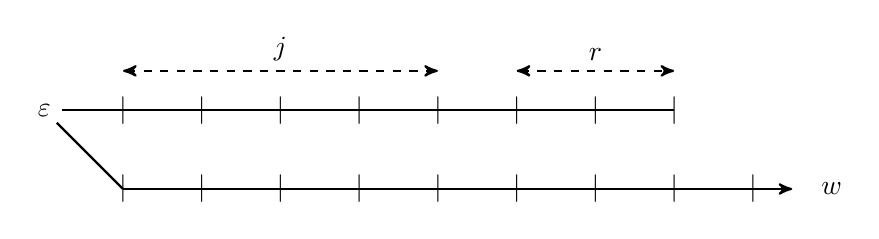
\begin{tikzpicture}[->,>=stealth',auto,thick, scale = 1.0,state/.style={circle,inner sep=2pt}]

    % The graph
    \node [state] at (0,0) (R) {$\varepsilon$};
    \node [state] at (1,0) (1) {$|$};
    \node [state] at (2,0) (2) {$|$};
    \node [state] at (3,0) (3) {$|$};
    \node [state] at (4,0) (4) {$|$};
    \node [state] at (5,0) (5) {$|$};
    \node [state] at (6,0) (6) {$|$};
    \node [state] at (7,0) (7) {$|$};
    \node [state] at (8,0) (8) {$|$};

    \node [state] at (0.9,-1) (ghost) {$$};
    
    \node [state] at (1,-1) (one1) {$|$};
    \node [state] at (2,-1) (one2) {$|$};
    \node [state] at (3,-1) (one3) {$|$};
    \node [state] at (4,-1) (one4) {$|$};
    \node [state] at (5,-1) (one5) {$|$};
    \node [state] at (6,-1) (one6) {$|$};
    \node [state] at (7,-1) (one7) {$|$};
    \node [state] at (8,-1) (one8) {$|$};
    \node [state] at (9,-1) (one9) {$|$};
    \node [state] at (10,-1) (one10) {$w$};
    
    \node [state] at (6.1,-1) (ghost2) {$$};
    
    % Graph branches

    \path[->]
    (1,-1) edge (9.5,-1);
    

    \path[-]
    (R) edge (1,-1)
    (ghost) edge (ghost2)
    (R) edge (8,0);

    
    \path[<->,dashed]
    (1,.5) edge node {$j$} (5,.5)
    (6,.5) edge node {$r$} (8,.5);
\end{tikzpicture} 
\caption{(Case a) Miner 1 forked at $\varepsilon$ successfully, since $r+j \leq \ell$.}
\end{figure}


We have
\begin{align*}
    \scriptsize    \frac{u_{a,j}(h)}{1-\beta} &\scriptsize =\sum_{\begin{array}{c}\scriptscriptstyle w\in \bstring\\ \scriptscriptstyle d\in \Dyck_{j-1}\\ \scriptscriptstyle |d| \leq 2\ell-j\end{array}}\beta^{|d|+j+1+|w|}\cdot \bigg(\alpha^{\frac{|d|+j}{2}+1} \cdot r(w)+\sum_{i=0}^{\frac{|d|+j}{2}}\alpha^{i+1} \bigg)\cdot h^{\frac{|d|+j}{2}+ 1}\cdot (1-h)^{\frac{|d|+j}{2}}\cdot \pr(w).
\end{align*}
Simplifying this expression yields
\begin{align*}
u_{a,j}(h) &= 
\frac{\alpha\cdot\beta\cdot h}{1-\alpha}\cdot x^j \cdot 
\bigg(\sum_{d\in \Dyck_{j-1}, |d|\leq 2l - j}x^{\frac{|d|-j}{2}}\cdot (1-\alpha^{\frac{|d|+j}{2}+1})\bigg)\\
& 
+\alpha\cdot\beta\cdot h \cdot(\alpha\cdot x)^j\cdot \bigg(\sum_{d\in \Dyck_{j-1}, |d|\leq 2l - j} (\alpha\cdot x)^{\frac{|d|-j}{2}}\bigg)\cdot\bigg(\sum_{w\in\bstring} \beta^{|w|}\cdot r_1(w)\cdot \pr(w)\bigg)\\
    &= \frac{\alpha\cdot\beta\cdot h}{1-\alpha}\cdot x^j\big(T_{j-1,\ell-j}(x)-\alpha^{j+1}\cdot T_{j-1,\ell-j}(\alpha\cdot x)) \;+\\
    &+ \alpha\cdot\beta\cdot h\cdot(\alpha \cdot x)^j\cdot T_{j-1,\ell-j}(\alpha\cdot x)\cdot u_1(\gup^k_\ell)(h),
\end{align*}
where $T_{n,m}$ is defined on section \ref{sec-trapezoid-pentagon}.

\end{subsubsection}

\begin{subsubsection}{Case (b)}
These states are of the form 
$$q = 0^j\cdot 1\cdot d\cdot 1\cdot w, d\in \Dyck_{k-1}, |d|+k \leq 2\ell, w\in \bstring.$$ 

\begin{figure}[ht!]

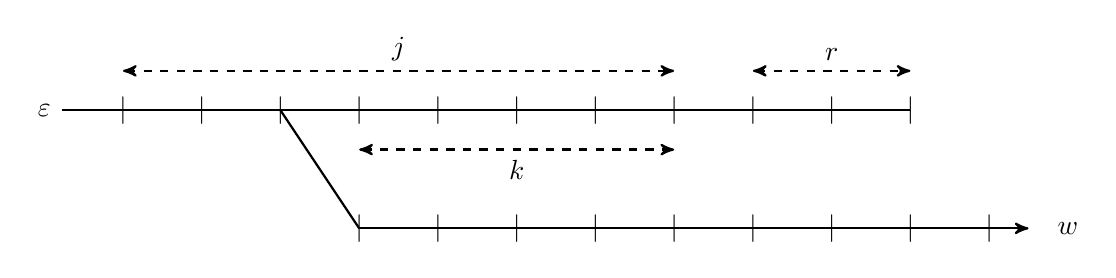
\begin{tikzpicture}[->,>=stealth',auto,thick, scale = 1.0,state/.style={circle,inner sep=2pt}]

    % The graph
    \node [state] at (-3,0) (R) {$\varepsilon$};
    \node [state] at (-2,0) (-2) {$|$};
    \node [state] at (-1,0) (-1) {$|$};
    \node [state] at (0,0) (0) {$|$};
    \node [state] at (1,0) (1) {$|$};
    \node [state] at (2,0) (2) {$|$};
    \node [state] at (3,0) (3) {$|$};
    \node [state] at (4,0) (4) {$|$};
    \node [state] at (5,0) (5) {$|$};
    \node [state] at (6,0) (6) {$|$};
    \node [state] at (7,0) (7) {$|$};
    \node [state] at (8,0) (8) {$|$};

    \node [state] at (0.9,-1.5) (ghost) {$$};
    
    \node [state] at (1,-1.5) (one1) {$|$};
    \node [state] at (2,-1.5) (one2) {$|$};
    \node [state] at (3,-1.5) (one3) {$|$};
    \node [state] at (4,-1.5) (one4) {$|$};
    \node [state] at (5,-1.5) (one5) {$|$};
    \node [state] at (6,-1.5) (one6) {$|$};
    \node [state] at (7,-1.5) (one7) {$|$};
    \node [state] at (8,-1.5) (one8) {$|$};
    \node [state] at (9,-1.5) (one9) {$|$};
    \node [state] at (10,-1.5) (one10) {$w$};
    
    \node [state] at (6.1,-1.5) (ghost2) {$$};
    
    % Graph branches

    \path[->]
    (1,-1.5) edge (9.5,-1.5);
    

    \path[-]
    (0,0) edge (1,-1.5)
    (R) edge (8,0);

    
    \path[<->,dashed]
    (-2,.5) edge node {$j$} (5,.5)
    (1,-.5) edge node[below] {$k$} (5,-.5)
    (6,.5) edge node {$r$} (8,.5);
\end{tikzpicture} 
\caption{(Case b) Miner 1 forked successfully, since $r+k \leq \ell$.}

\end{figure}

Analogously as before, we have
$$
 \scriptsize   \frac{u_{b,j}(h)}{1-\beta} = 
\scriptsize \!\!\!\!\!\sum_{
 \begin{array}{c}
 w\in \bstring\\
  d\in \Dyck_{k-1}\\
  |d| \leq 2\ell-k
  \end{array}
  }\!\!\!\beta^{\scriptscriptstyle j+|d|+k+1+|w|}\cdot \bigg(\alpha^{j-k}\cdot \bigg(\sum_{i=0}^{\frac{|d|+k}{2}}\alpha^{i+1}\bigg) + \alpha^{\frac{|d|-k}{2}+j+1} \cdot r(w)\bigg) \cdot h^{\frac{|d|+k}{2}+1}\cdot (1-h)^{\frac{|d|-k}{2}+j}\cdot \pr(w).
$$
Developing and simplifying this expression as the latter case yields
\begin{align*}
u_{b,j}(h) &= \frac{\alpha\cdot\beta\cdot h}{1-\alpha}\cdot \alpha^{j-k}\cdot \beta^{j+k}\cdot h^{k}\cdot (1-h)^{j}\big(T_{k-1,\ell-k}(x)-\alpha^{k+1}\cdot T_{k-1,\ell-k}(\alpha\cdot x)\big) \\
&+ \alpha\cdot\beta\cdot h\cdot \alpha^j\cdot\beta^{j+k}\cdot h^{k}\cdot(1-h)^{j}\cdot T_{k-1,\ell-k}(\alpha\cdot x)\cdot  u_1(\gup^k_\ell)(h).
\end{align*}

\end{subsubsection}


\begin{subsubsection}{Case (c)}
These states are of the form 
$$q = 0^j\cdot 1\cdot e\cdot w, e\in \Pent_{j-1,\ell-j+1}, w\in \bstring,$$ 
where $\Pent_{n,m}$ are all the binary strings with $m$ zeroes such that in every prefix, the number of ones minus the number of zeroes does not exceed $n$. The number of such strings is analyzed in section \ref{sec-trapezoid-pentagon}. Let us denote by $H(s)$ the Hamming weight of a binary string $s$. 

\begin{figure}[ht!]
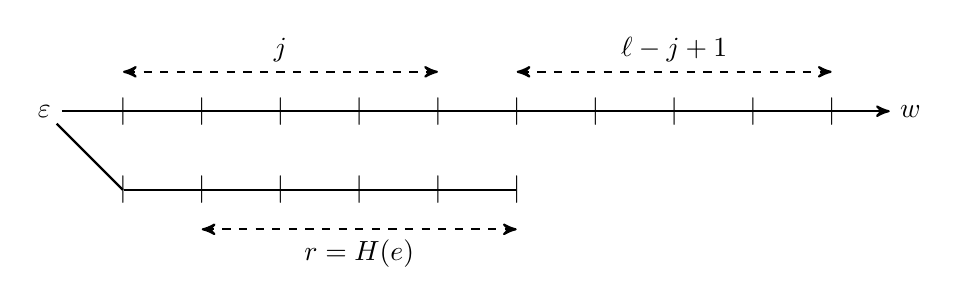
\begin{tikzpicture}[->,>=stealth',auto,thick, scale = 1.0,state/.style={circle,inner sep=2pt}]

    % The graph
    \node [state] at (0,0) (R) {$\varepsilon$};
    \node [state] at (1,0) (1) {$|$};
    \node [state] at (2,0) (2) {$|$};
    \node [state] at (3,0) (3) {$|$};
    \node [state] at (4,0) (4) {$|$};
    \node [state] at (5,0) (5) {$|$};
    \node [state] at (6,0) (6) {$|$};
    \node [state] at (7,0) (7) {$|$};
    \node [state] at (8,0) (8) {$|$};
    \node [state] at (9,0) (9) {$|$};
    \node [state] at (10,0) (10) {$|$};
    \node [state] at (11,0) (11) {$w$};
    \node [state] at (0.9,-1) (ghost) {$$};
    \node [state] at (1,-1) (one1) {$|$};
    \node [state] at (2,-1) (one2) {$|$};
    \node [state] at (3,-1) (one3) {$|$};
    \node [state] at (4,-1) (one4) {$|$};
    \node [state] at (5,-1) (one5) {$|$};
    \node [state] at (6,-1) (one6) {$|$};
    \node [state] at (6.1,-1) (ghost2) {$$};
    
    % Graph branches

    \path[->]
    (R) edge (11);
    

    \path[-]
    (R) edge (1,-1)
    (ghost) edge (ghost2);
    
    \path[<->,dashed]
    (1,.5) edge node {$j$} (5,.5)
    (6,.5) edge node {$\ell-j+1$} (10,.5)
    (2,-1.5) edge node [below] {$r=H(e)$}(6,-1.5);
\end{tikzpicture} 
\caption{(Case c) Miner 1 forked at $\varepsilon$ but gave up, since the upper branch attained $\ell$ blocks.}

\end{figure}

We have
\begin{align*}
u_{c,j}(h) &= (1-\beta) \cdot \sum_{w\in \bstring, e\in \Pent_{j-1, \ell-j-1}} \beta^{\ell+H(e)+|w|+2}\cdot \alpha^{\ell+1}\cdot r_1(w) \cdot h^{H(e)+1}\cdot(1-h)^{\ell+1}\cdot \pr(w).
\end{align*}
This yields the following:
\begin{align*}
u_{c,j}(h) &= \alpha\cdot x\cdot (\alpha\cdot\beta\cdot(1-h))^\ell\cdot u_1(\gup^k_\ell)(h) \cdot  \sum_{e\in\Pent_{j-1,\ell-j-1}}(\beta\cdot h)^{H(e)}\\
        &= \alpha\cdot x\cdot (\alpha\cdot\beta\cdot(1-h))^\ell \cdot P_{\ell,j}(\beta\cdot h) \cdot u_1(\gup^k_\ell)(h).
\end{align*}


\end{subsubsection}


\begin{subsubsection}{Case (d)}
These states are of the form $q = 0^j\cdot 1\cdot e\cdot w, e\in \Pent_{k-1,\ell-k+1}, w\in \bstring.$

\begin{figure}[ht!]
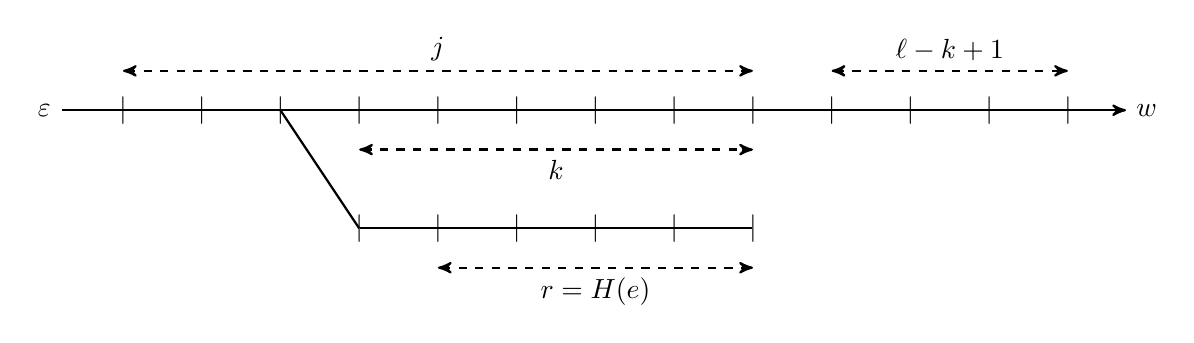
\begin{tikzpicture}[->,>=stealth',auto,thick, scale = 1.0,state/.style={circle,inner sep=2pt}]

    % The graph
    \node [state] at (-3,0) (R) {$\varepsilon$};
    \node [state] at (-2,0) (-2) {$|$};
    \node [state] at (-1,0) (-1) {$|$};
    \node [state] at (0,0) (0) {$|$};
    \node [state] at (1,0) (1) {$|$};
    \node [state] at (2,0) (2) {$|$};
    \node [state] at (3,0) (3) {$|$};
    \node [state] at (4,0) (4) {$|$};
    \node [state] at (5,0) (5) {$|$};
    \node [state] at (6,0) (6) {$|$};
    \node [state] at (7,0) (7) {$|$};
    \node [state] at (8,0) (8) {$|$};
    \node [state] at (9,0) (9) {$|$};
    \node [state] at (10,0) (10) {$|$};
    \node [state] at (11,0) (11) {$w$};
    \node [state] at (0.9,-1.5) (ghost) {$$};
    \node [state] at (1,-1.5) (one1) {$|$};
    \node [state] at (2,-1.5) (one2) {$|$};
    \node [state] at (3,-1.5) (one3) {$|$};
    \node [state] at (4,-1.5) (one4) {$|$};
    \node [state] at (5,-1.5) (one5) {$|$};
    \node [state] at (6,-1.5) (one6) {$|$};
    \node [state] at (6.1,-1.5) (ghost2) {$$};
    
    % Graph branches

    \path[->]
    (R) edge (11);
    

    \path[-]
    (0,0) edge (1,-1.5)
    (ghost) edge (ghost2);
    
    \path[<->,dashed]
    (-2,.5) edge node {$j$} (6,.5)
    (1,-.5) edge node [below] {$k$} (6,-.5)
    (7,.5) edge node {$\ell-k+1$} (10,.5)
    (2,-2) edge node [below] {$r=H(e)$}(6,-2);
\end{tikzpicture} 
\caption{(Case d) Miner 1 forked at some block, but gave up, since the upper branch attained $\ell$ blocks.}
\end{figure}


As in case (c), we compute
\begin{align*}
u_{d,j}(h) &= (1-\beta) \cdot \!\!\!\!\!\!\!\!\!\sum_{w\in \bstring, e\in \Pent_{k-1, \ell-k-1}}\!\!\!\!\!\!\beta^{\ell+j-k+H(e)+|w|+2}\cdot \alpha^{\ell+j-k+1}\cdot r_1(w) \cdot h^{H(e)+1}\cdot(1-h)^{\ell+j-k+1}\cdot \pr(w)\\
        &= \alpha\cdot x\cdot(\alpha\cdot\beta\cdot(1-h))^{j+\ell-k}\cdot P_{\ell,k}(\beta\cdot h) \cdot u_1(\gup^k_\ell)(h).
\end{align*}



\end{subsubsection}

Putting all of these expressions together and summing over $j$ gives an equation for $u_1(\gup^k_\ell)(h)$, that solves to the claimed rational function. More precisely, we have
$$u_1(\gup^k_\ell)(h) = u_0 + \sum_{j=1}^k (u_{a,j} + u_{c,j}) + \sum_{j=k+1}^\infty (u_{b,j} + u_{d,j}) = \Phi_{k,\ell} + \Gamma_{k,\ell}\cdot u_1(\gup^k_\ell)(h),$$
where $\Phi$ is the total contribution of one fork (successful or not) and $\Gamma$ is the total shifting factor. First note that $u_{b,j}+u_{d,j}$ is a geometric sequence in $j$ with a ratio in $[0,1)$, therefore the summation converges. In particular, $\Phi_{k,\ell}$ and $\Gamma_{k,\ell}$ are polynomials in $h$ whose coefficients depend in $\alpha,\beta,\ell,k$.
\end{proof}

\subsection{Trapezoidal and Pentagonal Dyck Polynomials}
\label{sec-trapezoid-pentagon}

In this section, we define two sets of polynomials that control the combinatorial nature of our game. They arise as generating polynomials of the sequences of states of fixed length. 

Recall that $\Dyck_{a,2b}$ is the set of binary strings of length $2b+a$ such that the number of ones equals the number of zeroes plus $a$, and such that for every prefix, the number of ones minus the number of zeroes is at most $a$. Now, define $\sigma_{a,b}:=|\Dyck_{a,2b}|$. Interpreting each 0 as a unitary $\uparrow$ step in $\ZZ^2$ and each 1 as a unitary $\rightarrow$ step, we have that $\sigma_{a,b}$ is the total number of $\{\uparrow,\rightarrow\}$ paths from $(0,0)$ to $(a,a+b)$ that lie within the trapezoid ${(0,0),(a,0),(a,a+b),(0,b)}$. We enumerate them in proposition \ref{enum-sigma}.

Also, from section \ref{sec-evaluation-G}, the set $\Pent_{a,b}$ consists of all binary strings with $b$ zeroes such that in every prefix, the number of ones minus the number of zeroes does not exceed $a$. Also, define $\Pent_{a,b}^r$ the number of such strings which have exactly $r$ ones, and define $\theta_{a,b}^r:= |\Pent_{a,b}^r|$. As before, note that $\theta_{a,b}^r$ is the total number of $\{\uparrow,\rightarrow\}$ paths in $\ZZ^2$ from $(0,0)$ to $(r,b)$ that lie within the pentagon $\{(0,0),(0,a),(r,r-a), (r,b), (0,b)\}$ (this is a rectangle if $r<a$). We develop a linear recurrence for $\theta_{a,b}^r$ that solves in terms of $\sigma_{a,b}$ in proposition \ref{enum-theta}. 

\begin{mydef}
For positive integers $n,m$, let
$$
\left\{
\begin{array}{lll}
T_{n,m}(x) &=& \displaystyle \sum_{i = 0}^{m} \sigma_{n,i}\cdot x^i\\
P_{n,m}(x) &=& \displaystyle \sum_{i = 0}^{m-1} \theta_{n-1,m-n+1}^i\cdot x^i
\end{array}
\right.
$$
\end{mydef}

This polynomials arise when evaluating utility for states with two branches. These states can be enumerated by length of the fork, and sums like the following arise (recall that $\Dyck_{n,2m}$ are the Dyck draws with disadvantage $n+2m$):
$$
\sum_{d\in \Dyck_{n}} x^{(|d|-n)/2} = \sum_{i=0}^m \sum_{d\in \Dyck_{n,2i}} x^{(|d|-n)/2} = \sum_{i=0}^m x^i\cdot  \bigg(\sum_{d\in\Dyck_{n,2i}} 1\bigg) = \sum_{i=0}^m x^i\cdot |\Dyck_{n,2i}| = T_{n,m}(x).
$$

For the sake of completeness, we compute closed forms for $\sigma_{a,b}$ and $\theta_{a,b}^r$ in the following section.



 \subsection{Trapezoidal and Pentagonal Dyck paths}
 \label{appendix-trapezoid}
 
 \subsubsection{Counting paths in a trapezoid.} For nonnegative integers $a,b$, let $\mathcal L_{a,b}$ be the trapezoid in $\ZZ^2$ whose vertices are
 $\{(0,0),(a,0),(a+b,b),(0,b)\}.$ Also, let $\mathcal{T}_{a,b}$ be set of one-step north-east paths from $(0,0)$ to $(a+b,b)$ that stay inside $\mathcal L_{a,b}$, and  $\sigma_{a,b}$ the amount of such paths. Finally, let $C_n$ denote the $n$-th Catalan number. 
 \begin{myprop}
    \label{sigma-recurrence}
    The sequence $\sigma:\NN^2\to \NN$ verifies the following recurrence:
    $$\begin{cases}
    \sigma_{a,b}=\sum_{i=0}^b\sigma_{a-1,i}\cdot C_{b-i}& \mbox{ for }a\geq 1,b\in \NN,\\
    \sigma_{x,0}=1 & \mbox{ for }x\in \NN,\\
    \sigma_{0,y}=C_y & \mbox{ for }y\in \NN.
    \end{cases}$$
 \end{myprop}
 \begin{proof}
    To prove this, we write $\mathcal T_{a,b}$ as a union of disjoint sets. As a first remark, note that every path in $\mathcal T_{a,b}$ touches the line $l=\overline{(a,0)(a+b,b)}$ at least once. For $i\in \{0,\dots,b\}$, let $P_i$ be the point $(a+i,i)\in l$ and $\mathcal T_{a,b}^{(i)}$ all paths in $\mathcal T_{a,b}$ that touch the line $l$ for the first time at $P_i$. We have the disjoint union
    $$\mathcal T_{a,b}=\bigcup_{i=0}^b \mathcal T_{a,b}^{(i)}.$$
    Also, note that a path in $\mathcal T_{a,b}$ touches $l$ for the first time in $P_i$ if and only if it passed through the point $P_i-(1,0)$ without exiting $\mathcal T_{a-1,i}$, followed by an east step and any path from $P_i$ to $(a+b,b)$. This yields
    \begin{eqnarray*}
        \sigma_{a,b}=\sum_{i=0}^{b}\mbox{(number of paths from $(0,0)$ to $P_i-(0,1))$}\cdot \mbox{(number of paths from $P_i$ to $(a+b,b))$}
    \end{eqnarray*}
    Note that the amount of paths from $P_i$ to $(a+b,b)$ is $C_{b-i}$, since both points belong to $l$, proving that $\sigma_{a,b}$ verifies the recurrence equation. The border cases $\sigma_{0,\cdot},\sigma_{\cdot,0}$ are straightforward to prove. 
 \end{proof}
 
 Now let us define the sequence of generating functions with respect to the second variable of $\sigma_{\cdot,\cdot}$ as follows:
 $$\begin{array}{cl}
 \phi_a:&\RR\to \RR\\
 &x\mapsto \displaystyle \sum_{j=0}^{\infty}\sigma_{a,j}\cdot x^j
 \end{array}$$
 
 \begin{myprop}
    For $x\in [0,1/4]$ and $a\in \NN$ 
    $$\phi_a(x)=c(x)^{a+1},$$
    where $c(x):=\frac{1-\sqrt{1-4x}}{2x}$ is the generating function of the Catalan numbers.
 \end{myprop}
 \begin{proof}
    We have $\sigma_{a,\cdot}=\sigma_{a-1,\cdot}\star C_\cdot$, where $\star$ is the convolution operator, therefore $\phi_a(x)=\phi_{a-1}(x)\cdot c(x)$. The result follows noting that $\phi_0(x)=c(x)$.
 \end{proof}
 
Extracting the sequence from the Taylor series of $\phi_a(x)$ around 0 and proving by induction gives
 \begin{myprop}
    \label{enum-sigma}
    For $(a,b)\in\NN^2$,
    $$\sigma_{a,b}=\frac{(a+b)\cdot(a+2b)!}{b!\cdot(a+b+1)!}=\frac{a+1}{a+b+1}\cdot {a+2b\choose a+b}.$$
 \end{myprop}


\begin{subsubsection}{Counting paths in a pentagon.} Let $\mathcal{P}_{a,b}^r$ be the set of north-east unitary-step paths from $(0,0)$ to $(r,b)$ that do not exit the pentagon $(0,0),(a,0),(r,r-a),(r,b),(0,b)$, and $\theta_{a,b}^r$ the amount of such paths. Also, let $\lambda$ be the diagonal line $\overline{(a,0)(r,r-a)}$. 
\begin{myprop}
    The sequence $\theta:\NN^3\to \NN$ verifies the following recurrence relation
    $$
    \displaystyle \theta_{a,b}^r = \theta_{a-1,b}^r + \sum_{i=0}^{r-a}\sigma_{a-1,i}\cdot \sigma_{a+b-r,r-a-i}.
    $$
 \end{myprop}
 \begin{proof}
 As in the proof of \ref{sigma-recurrence}, we write $\mathcal{P}_{a,b}^r$ as a disjoint union:

 \begin{align*}
 \mathcal{P}_{a,b}^r &= (\mbox{paths that do not touch }\lambda)\cup (\mbox{paths that touch }\lambda)\\
                     &= (\mbox{paths that do not touch }\lambda)\cup \bigcup_{y\in \lambda} (\mbox{paths that touch }\lambda\mbox{ for the first time at $y\in \lambda$})\\
                     &= (\mbox{paths that do not touch }\lambda)\cup \bigcup_{y\in \lambda} (\mbox{paths from }(0,0)\mbox{ to }y-(1,0))\cdot (1,0)\cdot (\mbox{paths from }y\mbox{ to }(r,b))\\
                     &= (\mbox{paths that do not touch }\lambda)\cup \bigcup_{i = 0}^{r-a} \begin{array}{l}(\mbox{paths from }(0,0)\mbox{ to }(a+i,i)-(1,0))\cdot\\ (1,0)\cdot (\mbox{paths from }(a+i,i)\mbox{ to }(r,b)),\end{array}
 \end{align*}
 where in the last equation, the symbol $\cdot$ stands for concatenation of paths. The recurrence follows noting that the paths that do not touch $\lambda$ are exactly $\mathcal{P}_{a-1,b}^r$, the paths from $(0,0)$ to $(a+i-1,i)$ are $\mathcal{T}_{a-1,i}$ and the paths from $(a+i,i)$ to $(r,b)$ are exactly $\mathcal{T}_{a+b-r,r-a-i}$. \end{proof}


 \begin{myprop}
 \label{enum-theta}
 For positive integers $a,b,r$ it holds that
 $$
 \begin{cases}
 \displaystyle\mbox{If }r\leq a,\quad \theta_{a,b}^r = {r+b\choose b},\\
 \displaystyle\mbox{If }a<r,\quad \theta_{a,b}^r = \sigma_{|b-r|,\min(r,b)} + \sum_{i=\max(1,r-b+1)}^a  \sum_{j=0}^{r-i}\sigma_{i-1,j}\cdot \sigma_{i+b-r,r-i-j}.\\
 %\displaystyle\mbox{If }a<r<b,\quad \theta_{a,b}^r = \sigma_{b-r,r} + \sum_{i=1}^a  \sum_{j=0}^{r-i}\sigma_{i-1,j}\cdot \sigma_{i+b-r,r-i-j},\\
 %\displaystyle\mbox{If }b<r\mbox{ and }a<r,\quad \theta_{a,b}^r = \sigma_{r-b,b} + \sum_{i=r-b+1}^a  \sum_{j=0}^{r-i}\sigma_{i-1,j}\cdot \sigma_{i+b-r,r-i-j},\\
 \end{cases}
 $$
 \end{myprop}
 \begin{proof}
    If $r\leq a$, the polygon is simply a rectangle from $(0,0)$ to $(r,b)$. If $a<r\leq b$, then the result yields adding the recurrence relation from the base case $a=0$ and noting that $\theta_{0,b}^r = \sigma_{b-r,r}$. If $b<r$, then the base case is $a=r-b$ and $\theta_{r-b,b}^r = \sigma_{r-b,b}$.
 \end{proof}
\end{subsubsection}


\end{document}
